\chapter{Cuantificadores de Aleatoriedad}

\section{Máximo Exponente de Lyapunov}
\label{sec:MLE}

El Máximo Exponente de Lyapunov (MLE) caracteriza que tan rápido se apartan dos trayectorias.
Si esta velocidad es exponencial, se dice que el sistema es caótico, por lo que este exponente es conocido como un detector de  ``caoticidad", \cite{strotgartz1994,Kantz1994,Sprott2003}.
Más adelante, el MLE fue utilizado en diversas aplicaciones de muy distintas áreas.
Sólo por mencionar alguna, en \cite{Ma2013} el MLE es usado para medir una señal muy débil en un gas ideal utilizando criterios caóticos.
En \cite{Bruijna2011}, se estudia si es posible predecir un cambio en la probabilidad de caída para un modelo simple de caminante humano a partir del $MLE$.

Los exponentes de Lyapunov son quantificadores que caracterizan como evoluciona la separación entre dos trayectorias \cite{Sprott2003}.
En general es bien conocido que el comportamiento caótico está principalmente caracterizado por los números de Lyapunov de la dinamica del sistema.
Si uno o mas números de Lyapunov es mayor que cero, entonces el sistema se comporta caóticamente, de otra forma el sistema es estable.

La distancia entre dos trayectorias cambia en $2^{MLE}$ por cada iteración, en promedio.
Si el $MLE<0$ las trayectorias se aproximan, esto puede deberse a un punto fijo.
Si el $MLE=0$ las trayectorias mantienen su distancia, esto puede deberse a un ciclo límite.
Si el $MLE>0$ la distancia entre las trayectorias es creciente, lo que es un indicador de caos.

Existe una forma no analítica de medir el $MLE$ si solo las entradas y las salidas de un sistema son accesibles.
El procedimiento es el siguiente: el sistema debe ser iniciado desde dos puntos cercanos en el plano de fase, llamémoslos $(x_a,y_a)$ y $(x_b,y_b)$.
A medida que el sistema es iterado se mide la distancia euclideana entre las dos trayectorias ($d_n$ en la muestra $n_{th}$) (eq. \ref{eq:D0D1}), y la trayectoria $b$ es relocalizada en cada iteración (eq. \ref{eq:reubicacion}) obteniendo los puntos $(x_{br},y_{br})$ para realimentar el sistema.
Entonces, el MLE puede ser calculado como se muestra en la ecuación \ref{eq:Lyapunov}.
El proceso puede verse en la Fig. \ref{fig:relocalizacion}.

\begin{eqnarray}\label{eq:D0D1}
d_{0(i-1)}&=& \sqrt{(x_{a(i-1)}-x_{br(i-1)})^2+(y_{a(i-1)}-y_{br(i-1)})^2}\nonumber\\
d_{1(i)}&=& \sqrt{(x_{a(i)}-x_{b(i)})^2+(y_{a(i)}-y_{b(i)})^2}\\
\nonumber
\end{eqnarray}

\begin{eqnarray}\label{eq:Lyapunov}
MLE &=& \frac{1}{n} \sum_{i=2}^{n} \log_2{\frac{d_{1(i)}}{d_{0(i-1)}}}
\end{eqnarray}

\begin{eqnarray}\label{eq:reubicacion}
x_{br(i)}&=& x_{a(i)}+(x_{b(i)}-x_{a(i)})d_{o(i-1)}/d_{1(i)} \nonumber\\
y_{br(i)}&=& y_{a(i)}+(y_{b(i)}-y_{a(i)})d_{o(i-1)}/d_{1(i)}
\end{eqnarray}

\begin{figure}
	\centering
	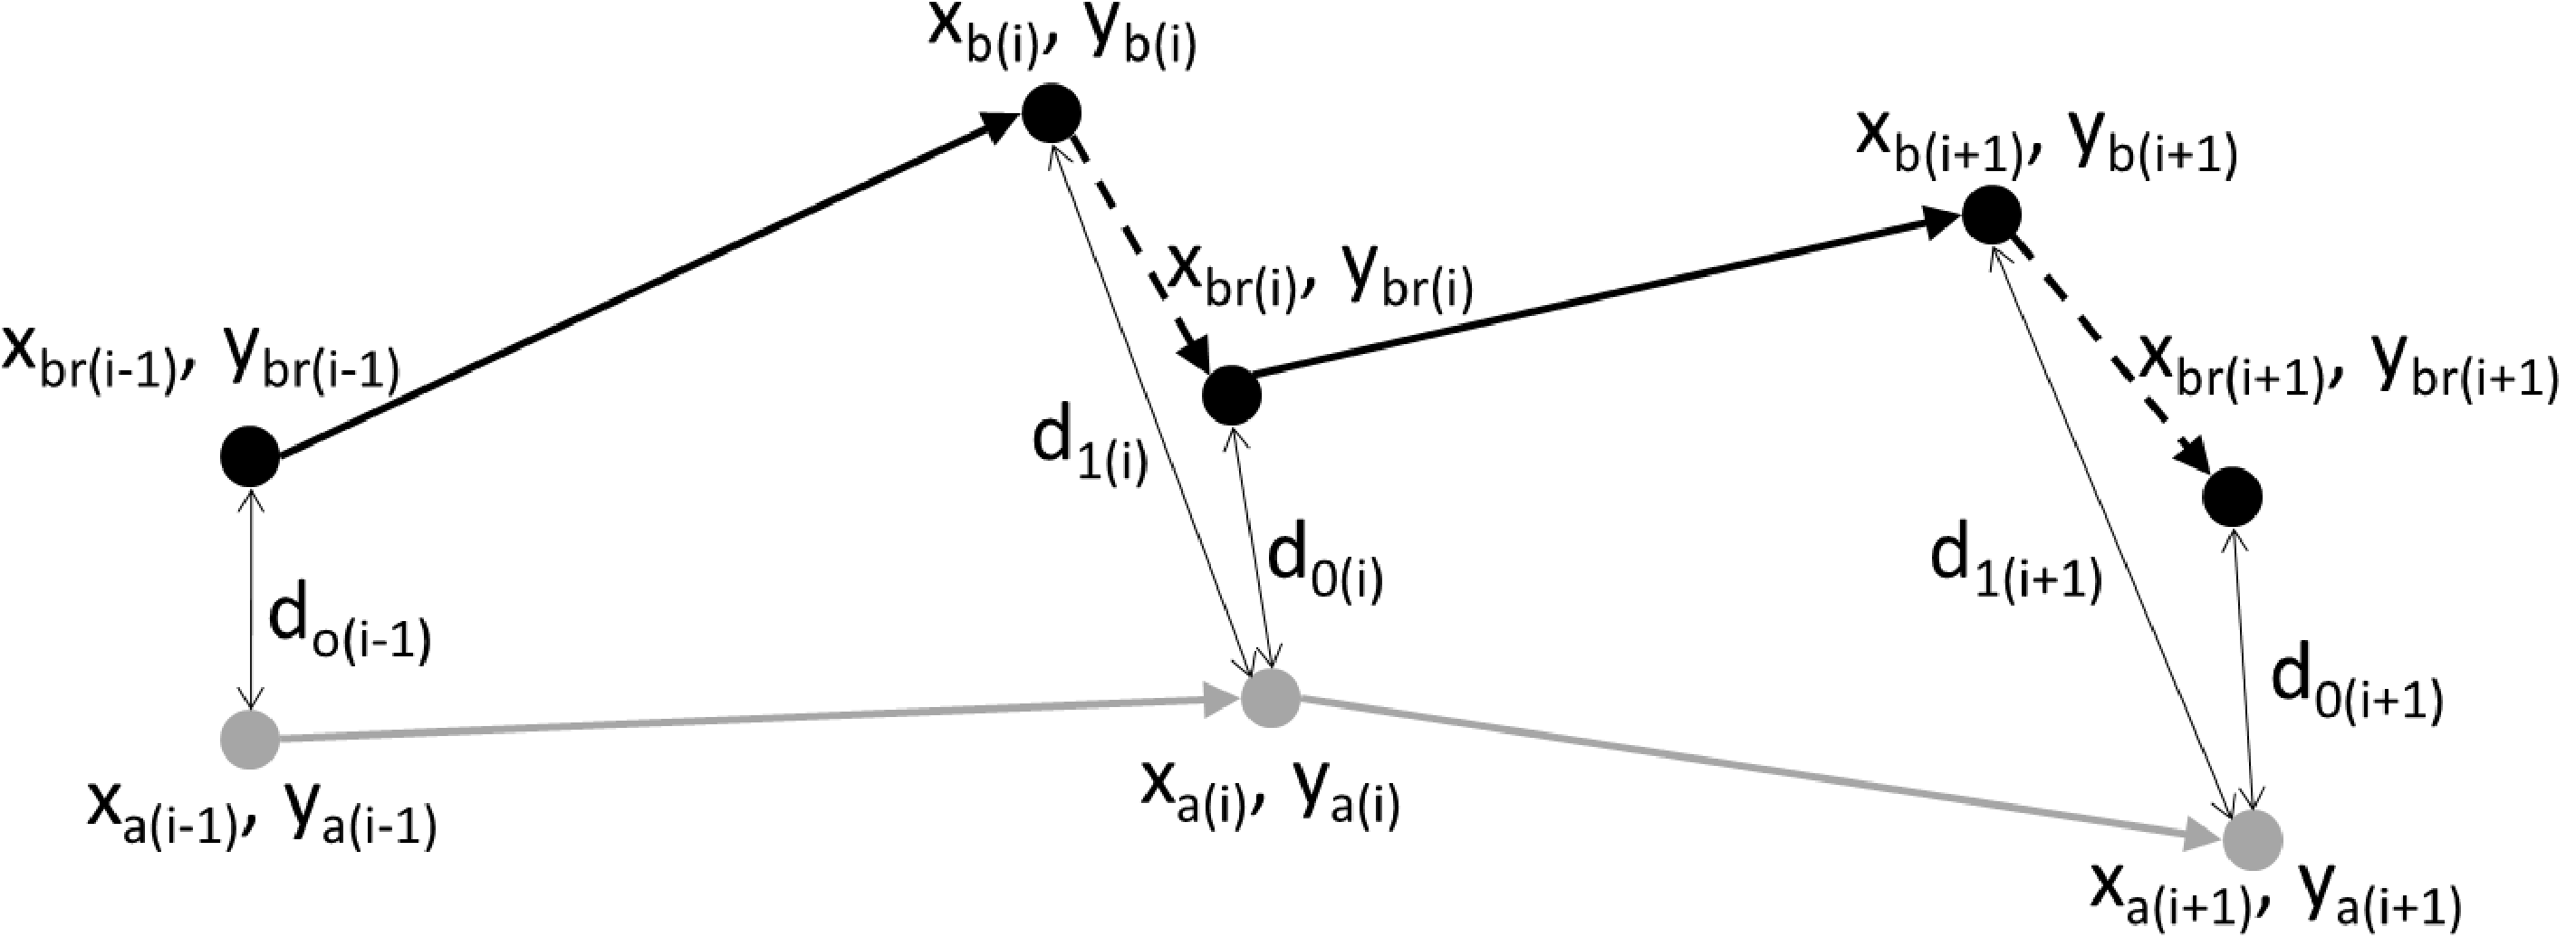
\includegraphics[width=1\columnwidth]{relocalizacion.pdf}\\
	\caption{Algoritmo para calcular el MLE.}\label{fig:relocalizacion}
\end{figure}



%%%%%%%%%%%%%%%%%%%%%%%%%%%%%%%%%%%%%%%%%%%%%%%%%%%%%%%%%%%%%%%%%%%%%%%%%%%%%%%%%%%%%%%%%%

\section{Causal and Non-causal Entropy quantifiers implemented in FPGA}

\subsection{Introduction}
\label{sec:Intro}
In the development of new electronic realizations of NonLinear Systems, specially Multiatractor chaotic Systems it is critical to be able to know and monitor the system's properties. Always a thorough analysis of the systems is required to meet the objectives, mainly the changes in the statistical properties induced by discretization of the system. Then it is necessary to check that the system still satisfies the application's requirements, this demands further analysis. Tools coming from the nonlinear analysis like Lyapunov exponents, cross, and autocorrelation, Perron-Frobenius operator, Correlation Dimension are employed, and also statistical tools like the Shannon Entropy, Complexity, Bandt and Pompe
embedding.

This work is part of a more ambitious project, which is the hardware development and implementation of tools for the analysis of nonlinear systems. These tools will mean a significant advance in the field of implementation of nonlinear systems. It will allow to more accurately understand and describe the behavior of the digital version of this type of systems. The complete package of tools that we intend to implement consists of:
\begin{itemize}
\item functional of the probability distribution: Shannon Entropy, Statistical Disequilibrium, and Statistical Complexity;
\item time series's quantifiers, especially Lyapunov exponents, autocorrelation, cross-correlation and fractal dimensions;
\item Perron-Frobenius operator, quantifiers of recurrent plots;
\item Statistical tests proposed in standardized banks for studying random number generators (Marsaglia, NIST, etc.).
\end{itemize}

At the moment, there is no much literature on hardware implementations of these tools \cite{DeMicco2013}.

In the particular case of entropy, it is used in various applications, such as in the anomaly detection of IP data flows \cite{Gu2005, Wagner2006}. In \cite{Subramanya2008} an FPGA design and simulation of an entropy quantifier is introduced, however currently there are no available hardware implementations of this quantifier.

Within the project mentioned in this paper a system that calculates the entropy of a particular probability distribution (PDF) associated with a data set is implemented. Causal and non-causal PDFs are analyzed. Data can have a digital source (generated by code) or can come from sampling external analog signals. The development board used the \textit{M1AFS-embedded kit}, based on the \textit{M1AFS1500} chip that is known for having an analog block embedded in the same package of the FPGA.

Then, the numerical accuracy of the implemented quantifier is verified  by comparing their results with a standard program. The maximum error detected determines the statistical accuracy of the system.

The organization of this paper is as follows: Section \ref{sec:entropias} both normalized entropies are presented for their consideration; Section \ref{sec:Hardware} describes the hardware implementation and interfaces; in \ref{sec:Software} the software is described in detail; Section \ref{sec:resultados} shows the obtained results of the system validation and in the measurement of the signals. In section \ref{sec:discusion}, experimental results are interpreted and discussed. Finally, we present our conclusions in Section \ref{sec:conclusiones}.

\subsection{Causal and Non causal Entropy}
\label{sec:entropias}
Let $X=\{x_i, i=1,...,N\}$ of length $N$ the output of a given source symbol, 
with alphabet $\mathcal{A}=\{a_i,i=1,...M\}$. Each element of $X$ is $x_i \in \mathcal{A}$.

The most commonly used \emph{PDF} is the normalized histogram of the $N$ values of $X$ between the $M$ symbols of $\mathcal{A}$; it is defined as $PDF_{hist}=\{p_i,i=1,...M\}$, where $p_i$ 
is the probability of occurrence of the symbol $a_i \in \mathcal{A}$. Its normalized Shannon entropy is referred to as   $H_{hist}$ and is defined:

\begin{equation}
\label{eq:entropia}
H_{hist}=\frac{\sum_{i=1}^{M}{p_i~log~p_i}}{logM}
\end{equation}

The standard entropy $H_{hist}$ quantifies the distribution of the elements of the series among all possible symbols.

If the source is a Pseudo Random Number Generator (PRNG), then all the symbols of the alphabet should appear the same number of times and its (optimal) value will be $H_{hist}=1$.

$PDF_{hist}$ is non-causal since it does not consider the temporal order of  time series' elements. This fact means that the $X$ vector could be rearranged to generate other vector $Y$, which would have the same histogram as $X$, and, therefore identical $PDF_{hist}$ and the same value for $H_{hist}$.

For quantifying statistical independence between consecutive elements, in this paper the causal PDF proposed by Bandt \& Pompe in \cite{Pompe2002} is used.
This PDF is obtained by assigning patterns of order to overlapped segments of length $D$ of the time series.

The process for its calculation is the following: first $D$ consecutive elements are grouped $\{x_i,x_{i+1},...,x_{i+D}\}$. Then the (ascending or descending) order of the $D$ values of each group is compared to the order of the vector $\{1,2,...,D\}$. There are $D!$ Possible ways to sort the numbers  $\{1,2,...,D\}$. If two values of $x_i$ within the same group are identical, it is considered that the first is lower, to obtain a unique result. Each permutation is called \emph{ordering pattern}\cite{Amigo2006}. 

The normalized histogram of the order patterns is the causal Bandt \& Pompe's PDF $PDF_{BP}$. The normalized Shannon entropy of that $PDF_{BP}$ is $H_{BP}$ where the subscript $BP$ means ``Bandt \& Pompe''.

Bandt and Pompe suggest $3\leq D \leq7$. For this work, we adopted $D=6$.

In the $H_{BP}$ vs. $H_{hist}$ plane \cite{DeMicco2008}, a higher value in any of the entropy values implies an increase in the uniformity of the involved $PDF$. The point $(1,1)$ represents an ideal case were both distributions, distribution of values and distribution of order patterns, are uniform.

A complete discussion about the convenience of using these quantifiers is beyond the scope of this work. A broad study can be found in \cite{DeMicco2008,Wackerbauer1994,Lopez1995,Rosso2007A,Rosso2009}.

\subsection{Implemented Hardware}
\label{sec:Hardware}

The hardware design was based on ACTEL's configuration on the 8051 microcontroller, and peripheral interfaces. It was developed using the software package \textit{Libero~Soc~v11.3\textsuperscript\copyright}. The development board used was \textit{M1AFS-EMBEDDED-KIT} that contains an FPGA \textit{M1AFS1500} and peripherals \cite{actelM1AFS1500}.

The \textit{M1AFS1500} embedded chip contains an analog block consisting of nine addressable adapters of four inputs each, a 32 inputs analog multiplexer and a configurable analog-digital converter.

For handling this block, a system also provided by ACTEL is used. This system is based on an 8051 microcontroller, and it  also contains drivers of the peripheral among other things \cite{Core8051sS,Core8051sH}.

The developed system can be divided into three main stages as shown in Fig. \ref{Fig:Sistema}: the first phase is the Acquisition, which converts the incoming analog signals into digital words. The next step is the Calculation logic stage, it uses the SRAM to perform calculations and coordinate the interfaces, and the last stage is the Presentation which sends the results to a computer through the USB-to-UART interface.

\begin{figure}
 \centering
 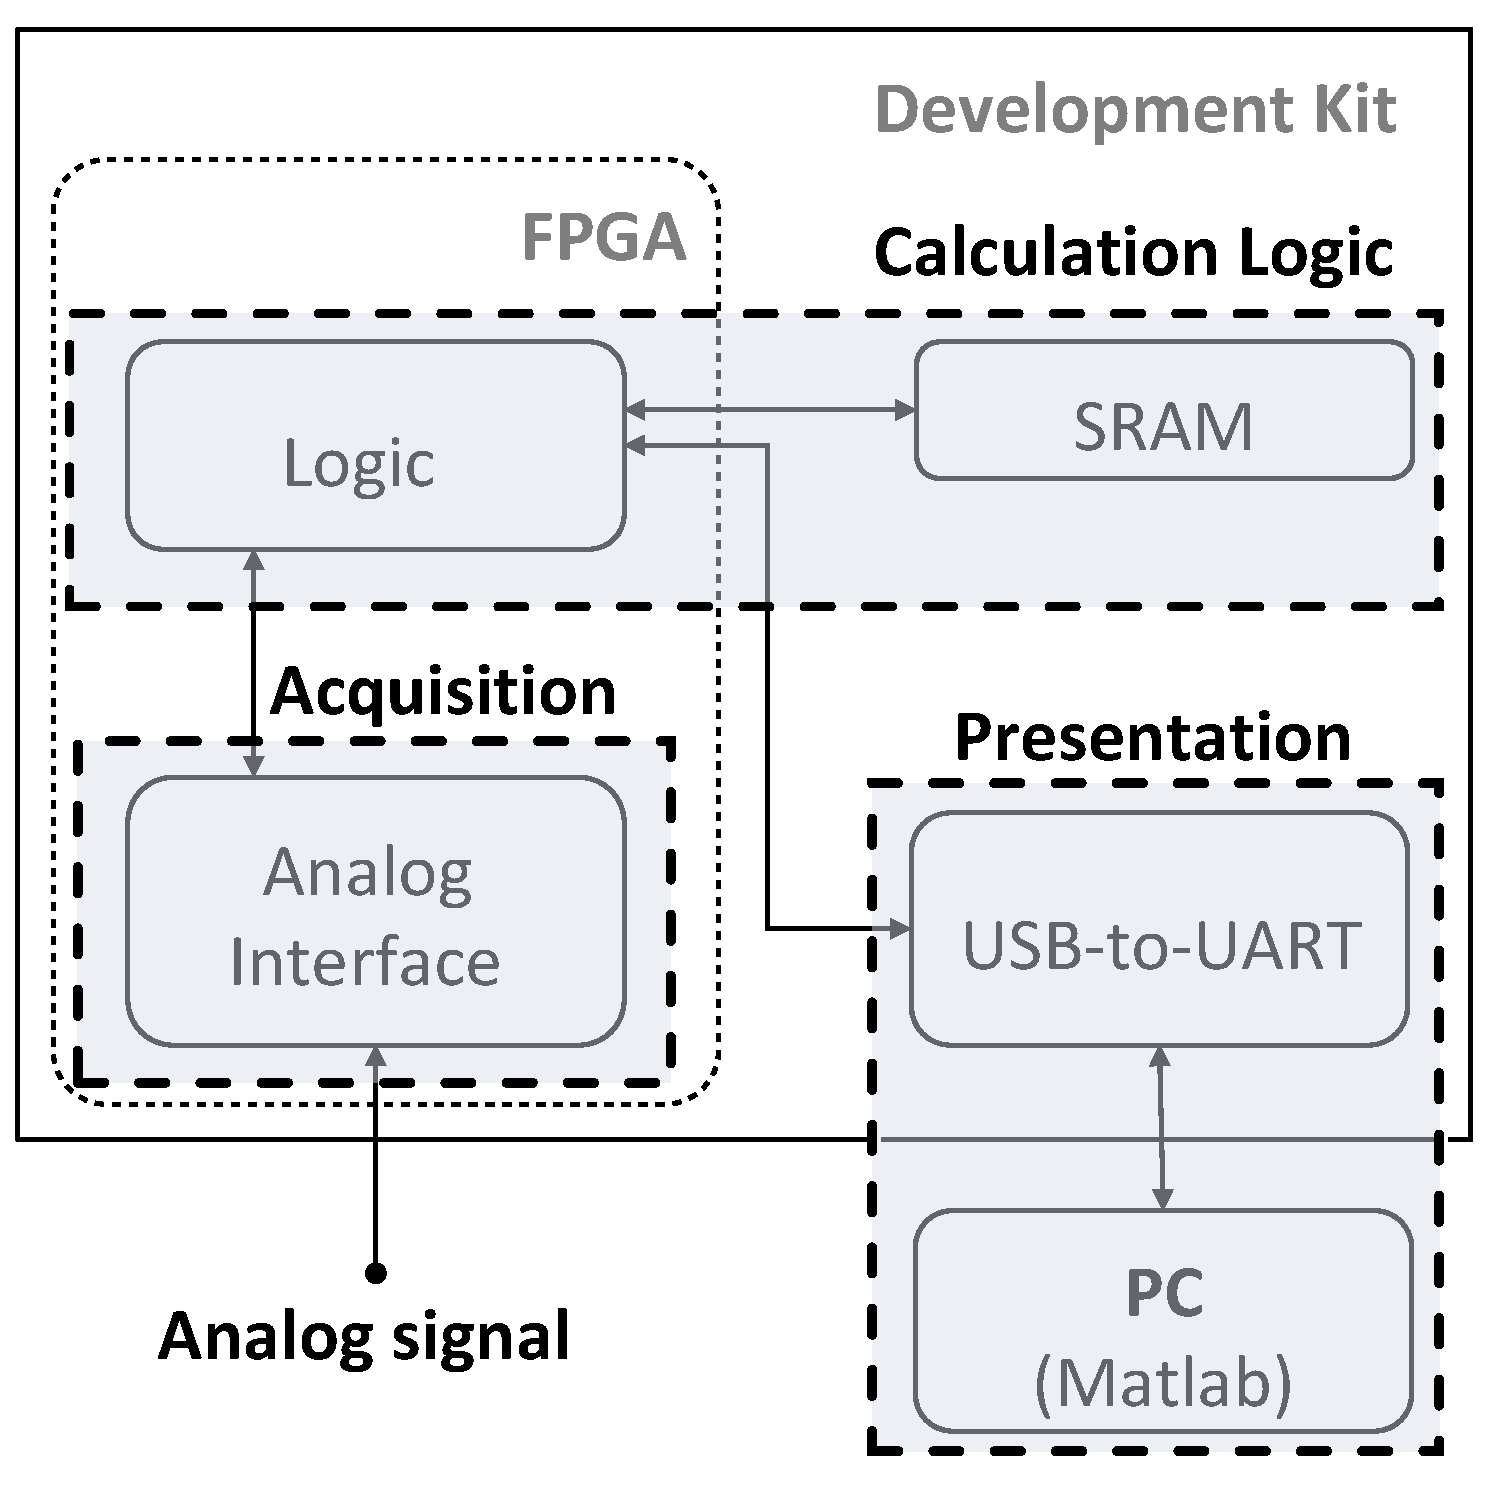
\includegraphics[width=.8\columnwidth]{Sistema_edit.pdf}\\
 \caption{Scheme of the complete system.}\label{Fig:Sistema}
\end{figure}
%
\subsubsection{Acquisition Stage}
%
The analog data to be evaluated is entered into the system by using the voltage input $AV2$ of the analog block \textit{Analog~Quad~2}. 
This input is mapped to channel seven of the analog multiplexer, and it was configured with an input voltage of 0~V to 4~V.
The analog-digital converter was configured with a 12-bit resolution. In this first prototype the maximum sample rate achieved was 16~ks/s, limited by the processing logic delay. This speed was enough for the required measurements. However, in a next stage an optimization of the design will be developed by increasing the operating frequency, among other improvements.

\subsubsection{Calculation logic}
%
The calculations and synchronization between peripherals are made at this stage. Figure \ref{fig:logica} shows the main blocks that compose it.

\begin{figure}
 \centering
 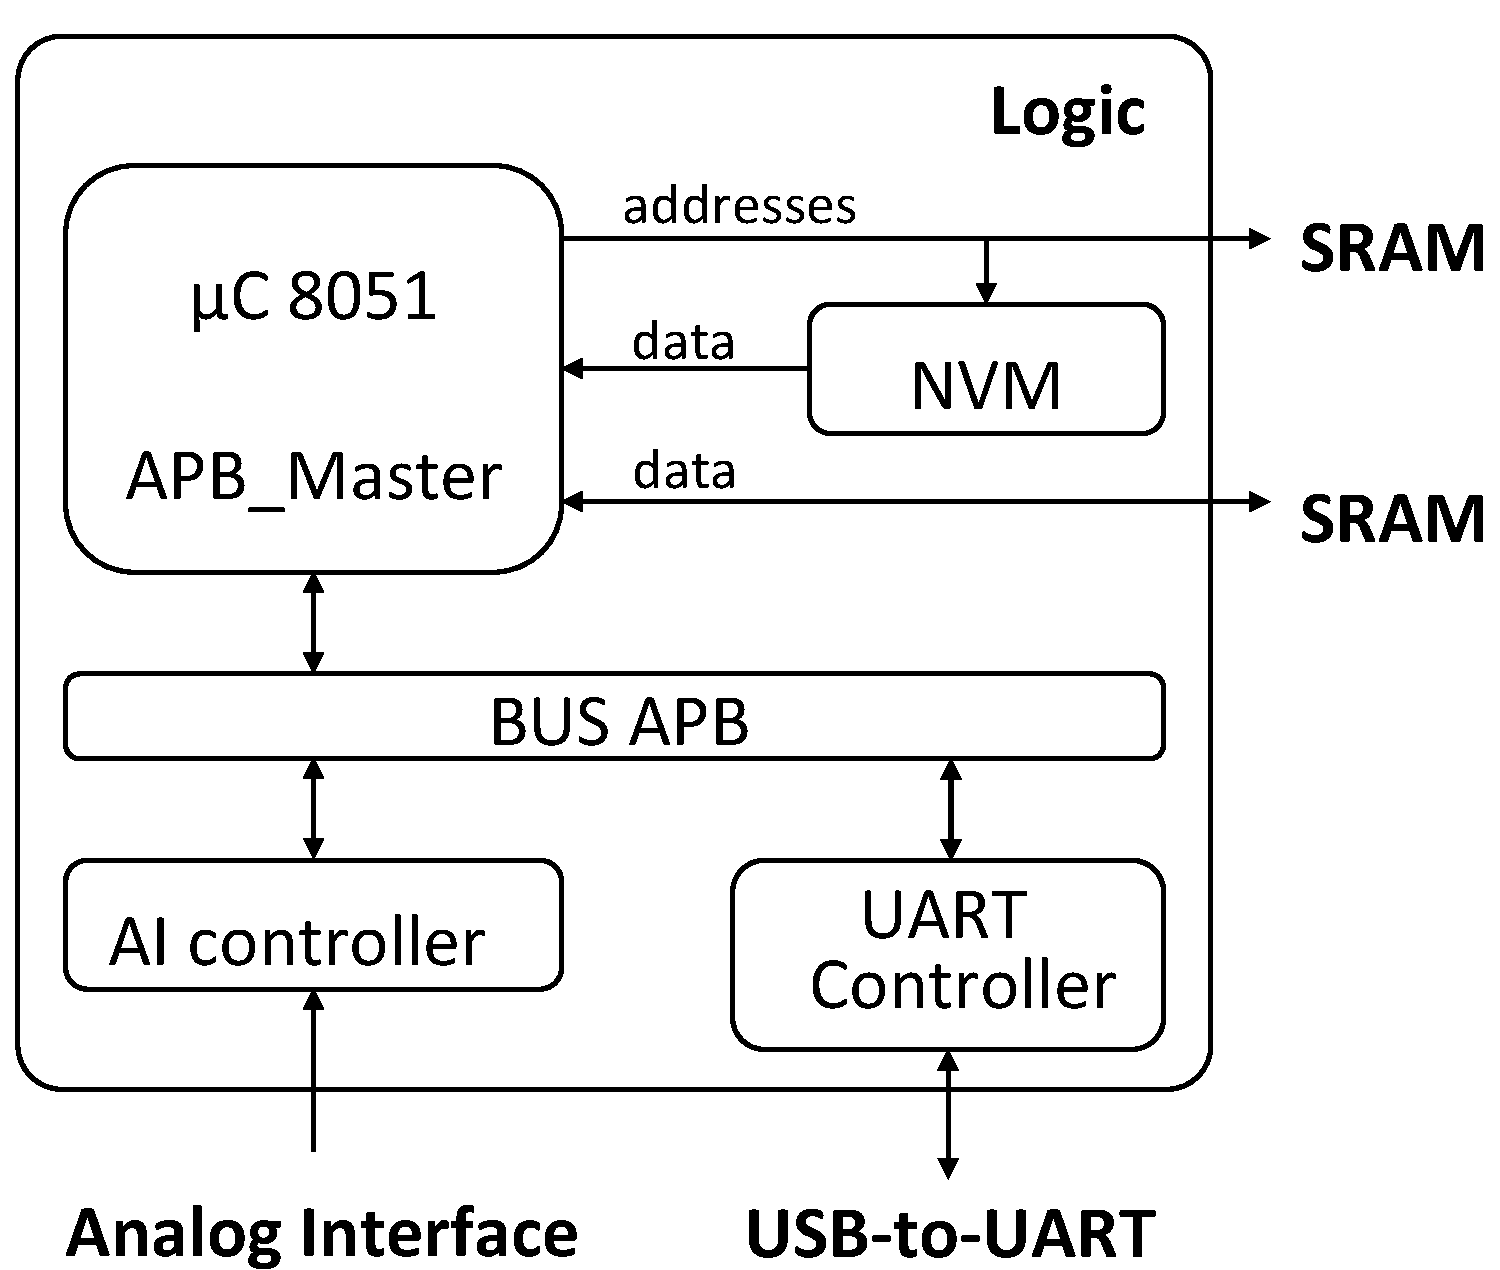
\includegraphics[width=.85\columnwidth]{Logica_edit.pdf}\\
 \caption{Details of the Calculation Logic stage.}\label{fig:logica}
\end{figure}

The heart of implementation is an 8051 Core that provides  Actel in its library catalog. It is a microcontroller containing the central logic of the Intel 8051 microprocessor, without its peripherals.
This micro has a Harvard architecture with a 16~bits address bus, limiting our design to 64~KB of memory code and 64~KB of data memory.

The application that performs the calculations presented in section \ref{sec:entropias} runs over this microcontroller.
It is responsible for obtaining the PDFs (BP and hist) and to perform the calculations to get the entropies from the input data, according to Eq. \ref{eq:entropia}. Section \ref{sec:Software} describes in detail the developed software.
In this particular FPGA, the code memory is a non-volatile memory (NVM) and is implemented in the internal flash of the FPGA blocks. It is mapped onto the addresses from 0x0000 to 0xFFFF and is written  during compilation with the contents of a hexadecimal format file.

The system functionality is extended by connecting peripherals through the APB interface.

For handling communication with the PC, the UART controller is used. The output of this block is directed out of the FPGA and is connected to a USB-to-UART chip that is soldered to the board.
The analog block is controlled by the AI controller, which routes and synchronizes its inputs.

%
\subsubsection{Presentation}
The stage of data presentation involves the USB-to-UART chip adapter that is on the development board and is driven both by the program running on the FPGA as well as by the software that runs on the PC. 

The USB-to-UART chip is responsible for adapting the input-output UART logic to an input-output USB standard by which is possible to interact with the PC. Moreover, the program running on the PC handles the user interface and is described in detail in the next section.

\subsection{Implemented Software}
\label{sec:Software}

The system operation is achieved by the interaction of two programs. One running on the PC and another on the microcontroller instantiated in the FPGA. It can be seen a flow chart of the two programs and the interaction between them in Fig. \ref{fig.softflow}.
%
\begin{figure}[htpb]
\centering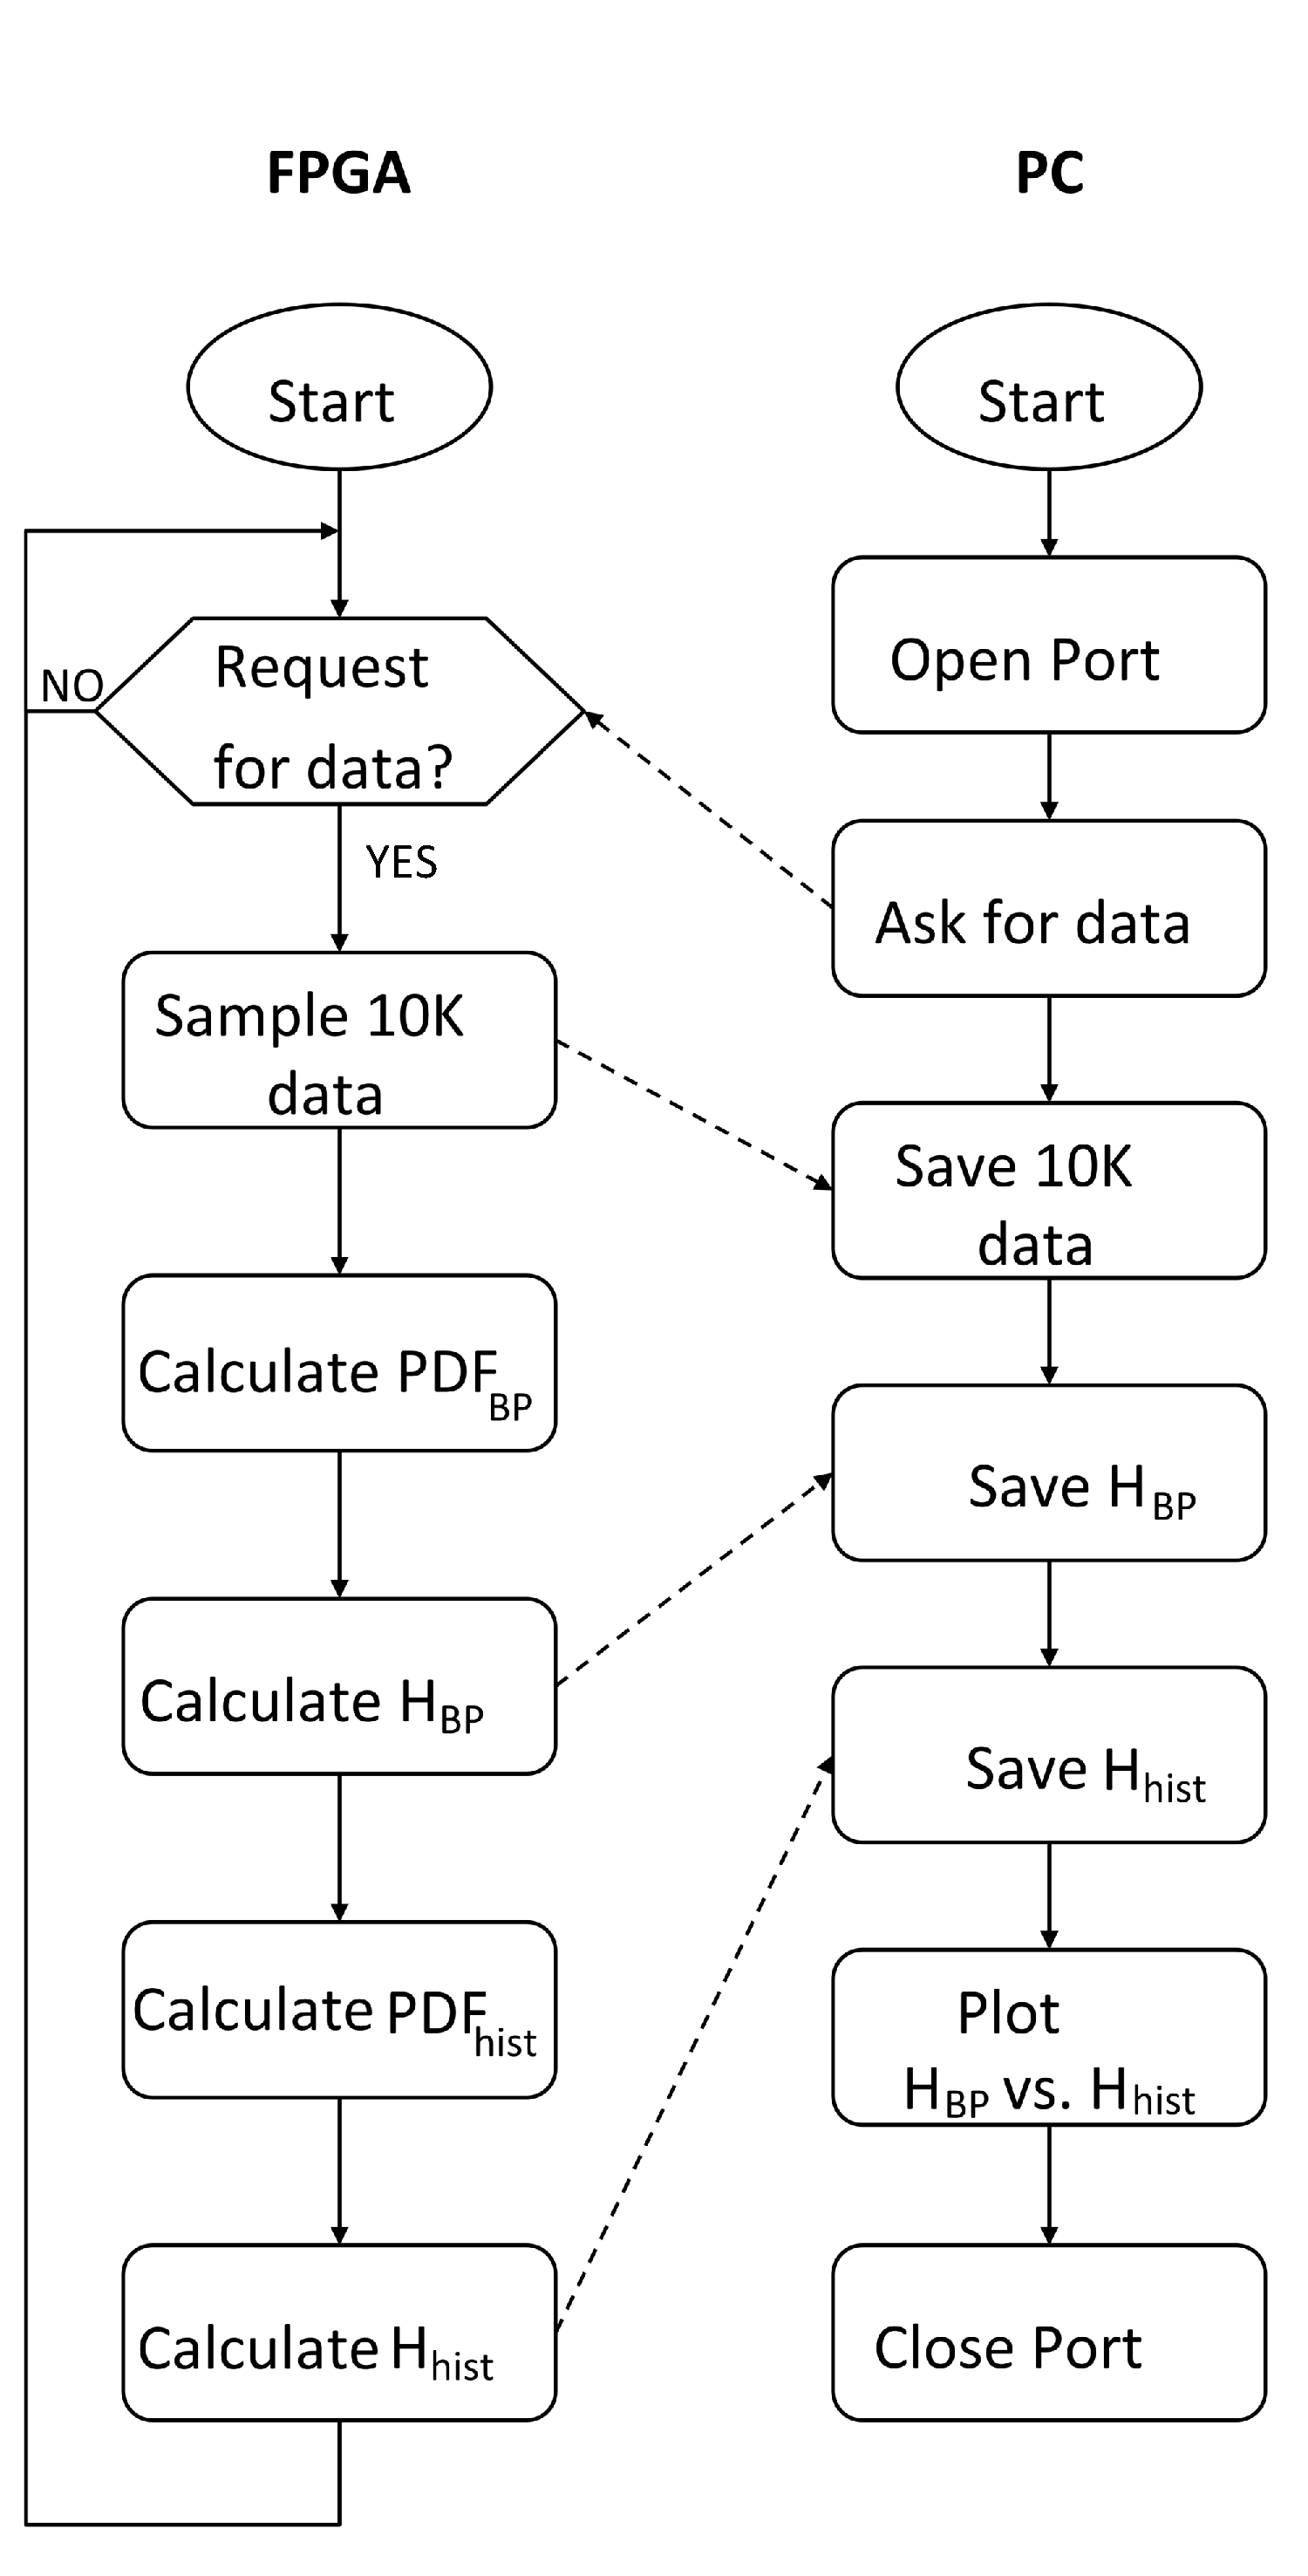
\includegraphics[scale=0.23]{Soft_edit2}
\caption{Flowchart of the implemented software.}\label{fig.softflow}
\end{figure}
On the PC runs a Matlab's script that is responsible for opening the serial port where the USB is mapped, requesting data, taking the results of the port, then plotting them in a plane $H_{BP}$ vs. $H_{hist}$ and finally closing the port.

Over the microcontroller instantiated in the FPGA runs a program written in C language and compiled for the 8051 microcontroller using the \textit{SoftConsole~IDE~v3.4\textsuperscript\copyright} tool. The firmware used is a modification of \cite{Core8051sS}. When a request for data from the UART port occurs, the data sampled in the analog input are stored. Then, $PDF_{hist}$ y $PDF_{BP}$ are calculated, and with this information, their respective entropies $H_{hist}$ and $H_{BP}$ are also calculated. These results are sent to the PC through the same port.

To validate the system, and verify how accurate the results are, the incoming sampled vector data is forwarded to the PC, so that it can calculate their entropies with PC using \textit{Matlab\textsuperscript\copyright} and compare them with the results of the implemented system.

\subsection{Results}
\label{sec:resultados}
As said, to test the system, the obtained results were compared with the results achieved by a pattern program running on the PC. For this, $10000$ samples of different waveforms were generated by both external (analog) and internal (digital) signals.

Two digital signals were produced by the code in the microcontroller, one corresponds to the rand() C function and the other to the chaotic Logistic map with parameter $r=4$.

Analog signals were generated with the \textit{HP33120A} waveform generator. With a range of $4~Vpp$ and $2~V$ of direct current to take advantage of the full spectrum of the analog-digital converter and increase the signal to noise ratio. In all four cases, the signal frequency was $100~Hz$ and the sampling rate of $16~ks/s$.

Table \ref{tabla} shows the absolute error between the calculated results of the quantifiers in the FPGA compared with the results calculated with the standard program running on the PC, over the same samples.

\begin{table}
\centering
\caption{Quantifiers error evaluated in the FPGA with respect to the results calculated by the pattern program.}\label{tabla}
\begin{tabular}{@{\extracolsep{\fill}}| c| c | c |c |}
 \hline
 \textbf{Generator} & \textbf{Source} & \textbf{Error $H_{BP}$} & \textbf{Error $H_{hist}$} \\
 \hline
Rand & Digital & $1,7421E^{-6}$ & $2,6977E^{-6}$ \\
 \hline
Logistic & Digital & $0,4256E^{-6}$ & $94,693E^{-6}$ \\
 \hline
Triangular & Analogic & $6,3445E^{-6}$ & $2,0028E^{-6}$ \\
 \hline
Sinusoidal & Analogic & $6,3151E^{-6}$ &$5,6506E^{-6}$ \\
 \hline
Square & Analogic & $0,1797E^{-6}$ & $1,9930E^{-6}$ \\
 \hline
Ramp & Analogic & $245,00E^{-6}$ & $1,0876E^{-6}$ \\
 \hline
\end{tabular}
\end{table}

Fig. \ref{fig:resultados} shows in the $H_{BP}$ vs. $H_{hist}$ plane the results calculated by the FPGA.

\begin{figure}[htb]
\centering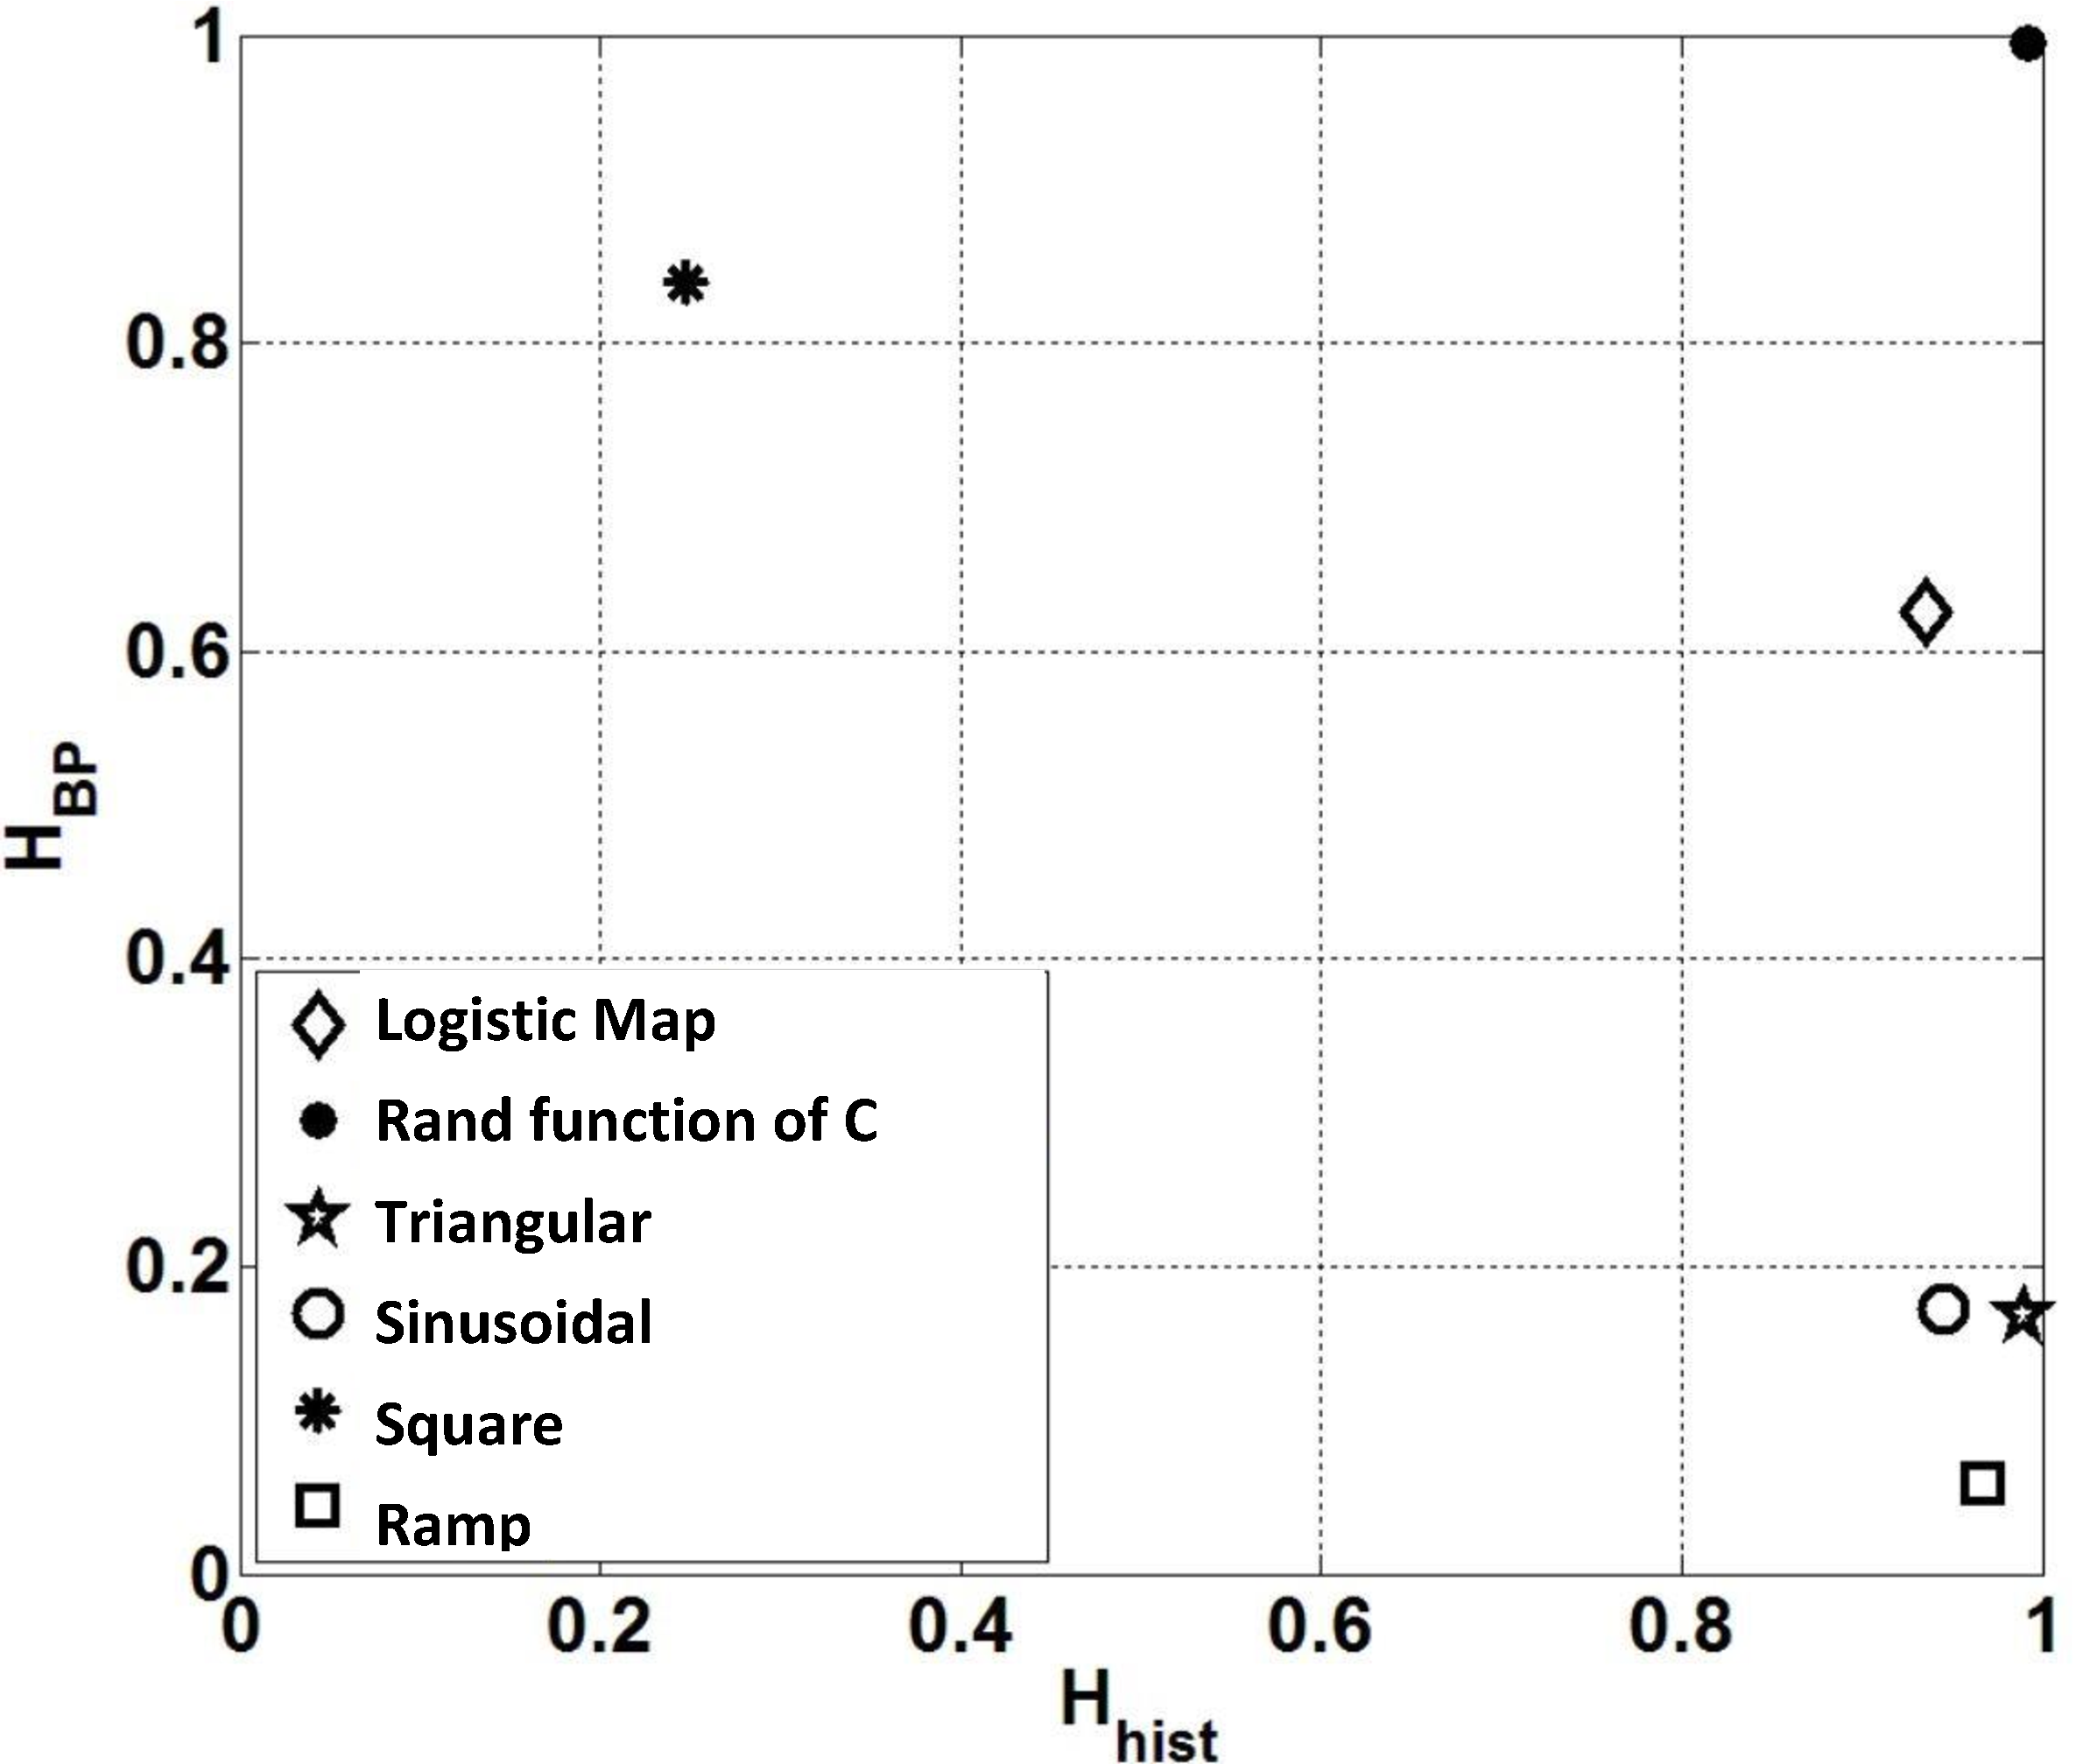
\includegraphics[height=0.26\textheight]{resultados_edit}
\caption{Measurement results.}\label{fig:resultados}
\end{figure}

Compilation results show the FPGA resources needed by the entire system and also the amount of memory occupied by the software running on the microcontroller. It is important to highlight that this is a rigid hardware implementation, i.e. the first circuit in the FPGA (microcontroller, peripheral, etc.) are configured and then the software is loaded on it.
The report returned after running the ``Place and Route" tool is shown in Fig. \ref{fig:hard}. 
It can be seen that the implementation uses 19\% of the FPGA logic resources, 21\% of the input-output cells and 28\% of the memory blocks.

The compilation report of the software part of the system is shown in Fig. \ref{fig:soft}. We can see that the non-volatile flash memory is 15.4\% occupied. 

On the other hand, of the $65536$ addresses the SRAM have available just $61440$ because some of this addresses are used by the APB bus, so the $76.7\%$ of the available memory is used.
%
\begin{figure}[htb]
\centering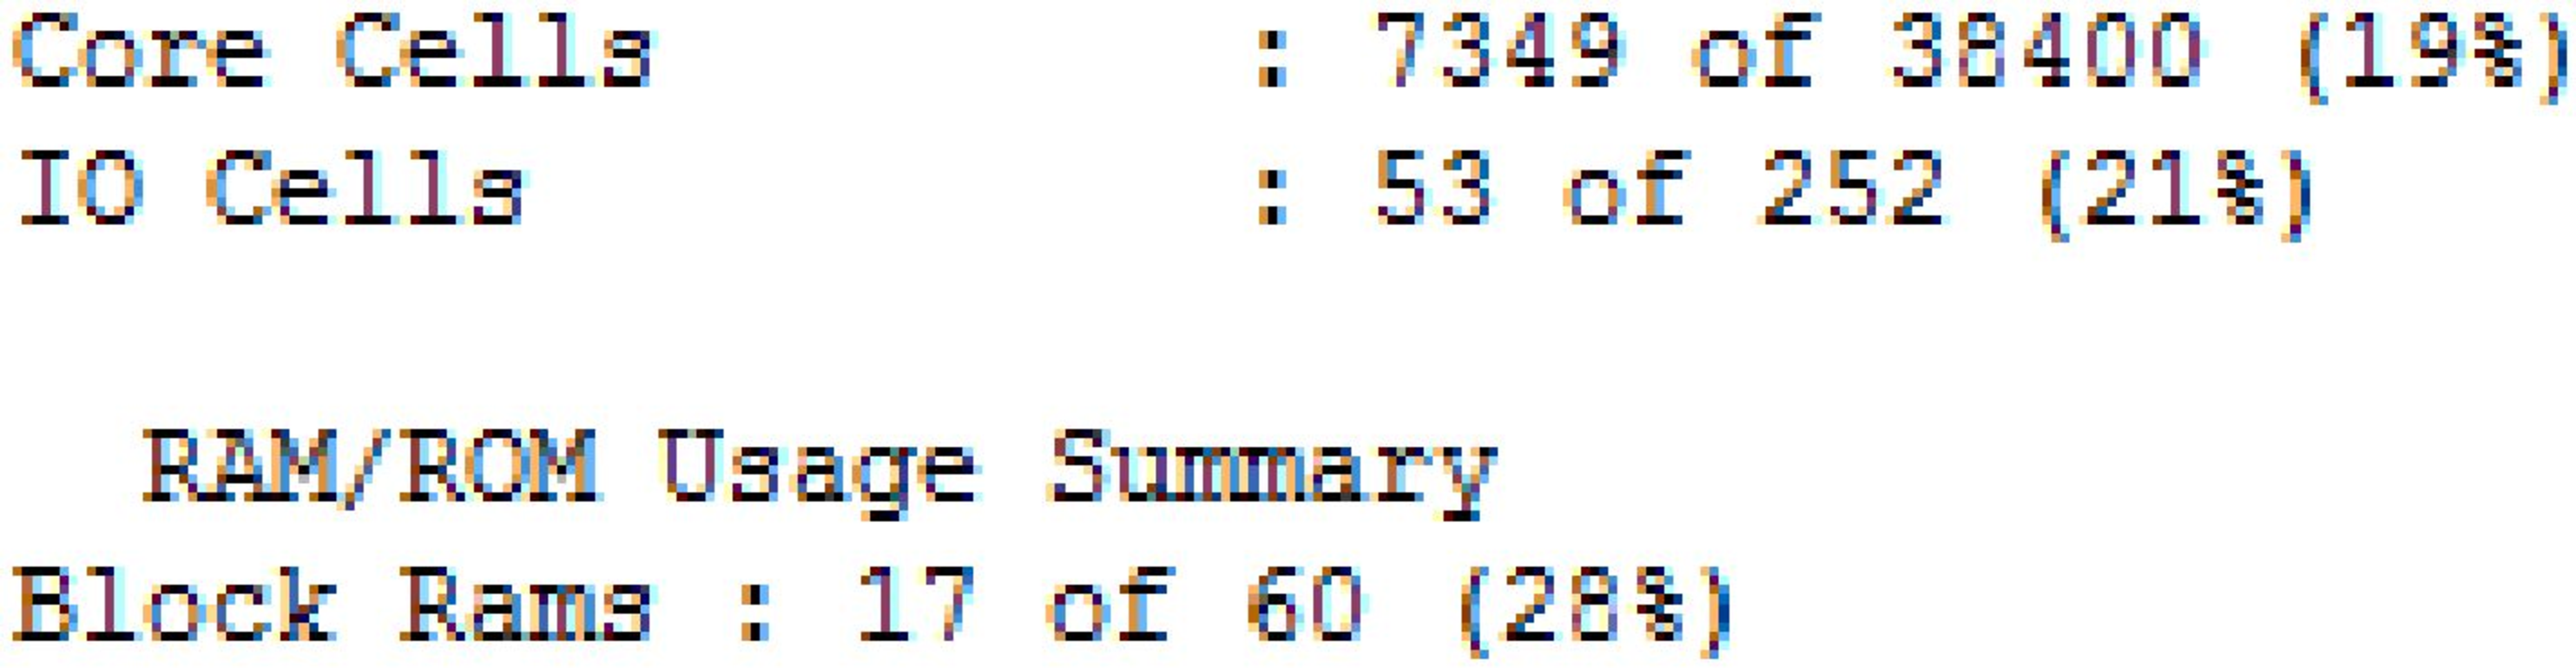
\includegraphics[scale=.13]{reporteHard}
\caption{Resources used by the system hardware.}\label{fig:hard}
\end{figure}

\begin{figure}[htb]
\centering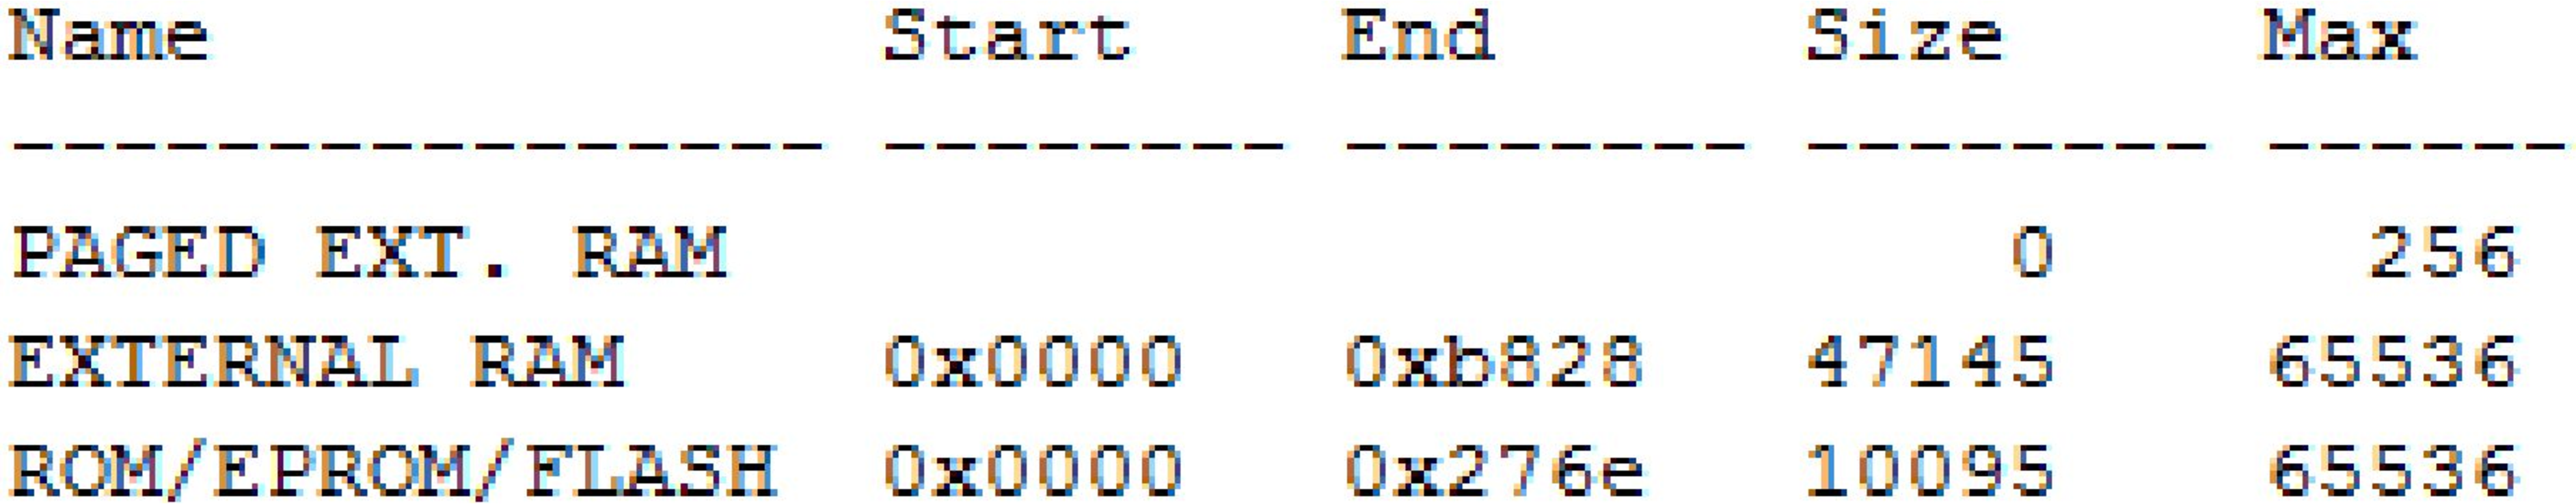
\includegraphics[scale=.13]{reporteSoft}
\caption{Resources used by the system software.}\label{fig:soft}
\end{figure}

\subsection{Discussion}
\label{sec:discusion}
%
The software had to be adapted to the microcontroller instantiated in the FPGA. 
The pattern program uses 64-bit floating point arithmetic (IEEE754-64~bits standard ) and uses the math.h library \cite{Mathe}.
For adapting the algorithm to be able to implement it in the  microcontroller that was instantiated in the FPGA, we had to reduce the number of bits employed. We used 32-bit floating point arithmetic (IEEE754-32~bits standard). The calculation of the logarithm function was also required, so it was implemented using the CORDIC algorithm. 
These differences make the output of the implemented system not to be equal to that of a program running on the PC, which we take as pattern program. Thus, these differences were measured, to have a dimension and determine whether the results are correct.

Table \ref{tabla} shows that the absolute error never exceeds the value $245E^{-6}$. This boundary indicates that there is a difference from the fifth decimal digit.

It can be seen in Fig. \ref{fig:resultados} that $H_{BP}$ and $H_{hist}$ quantifiers can clearly  difference between the statistical properties of the analyzed data.
Sinusoidal, Ramp and triangular signals have the highest values for $H_{hist}$ because the present all the possible values that the Analog-digital converter can generate.

However, the mixing of these signals are not good because they are periodic signals, so they are totally predictable, this is reflected by the small values of $H_{BP}$.
An interesting case to be analyzed is the square signal. The additive noise effect is specially marked in the areas where the value of the signal should be constant.

Two very narrow Gaussian curves appear around the ideal values of the $PDF_{hist}$, this does not affect too much the calculated value of $H_{hist}$, however for $PDF_{BP}$, the order pattern is derived directly from the noise, with a particular mean value, so the value of $H_{BP}$ will be higher than expected.

The signal generated by rand function of C has the best statistical properties being located at the point $\sim(1,1)$.

\subsection{Conclusions and future work}
\label{sec:conclusiones}
%
It was developed and implemented a system that allows a measurement with the proper precision of the causal and non-causal entropy of external analog signals from the outside of the FPGA and internal signals generated by code.
It was possible to measure signals and perform complex calculations with a small microcontroller as the 8051  instantiated in ACTEL AFS1500 FPGA. This first prototype meets the required specifications of accuracy and the quantity of resources established in the design. The following step will be to optimize the system regarding operating frequency and noise immunity.
It is expected that the system will allow modifying, at runtime, the sampling rate, so it would be adaptable to the input signal, with the upper limit of $500~Ks/s$ set by the ADC.

A threshold level should be added from which a value will be considered different from another, thus, the problem with the additive noise in the calculation of $H_{BP}$ will be solved.
The code for this system occupies $15.4\%$ of the total flash memory of the instantiated micro, so it will be possible to add software to implement other quantifiers and functionalities. As for the issue of the resources available in the FPGA, the logic cells used is $7349$, leaving almost $80\%$ of the available hardware resources to implement the systems under test, concurrently with the quantifiers.



%%%%%%%%%%%%%%%%%%%%%%%%%%%%%%%%%%%%%%%%%%%%%%%%%%%%%%%%%%%%%%%%%%%%%%%%%%%%%%%%%%%%%%%

\section{Measuring the Jitter of Ring Oscillators by means of Information Theory Quantifiers}

\subsection{Introduction}
\label{sec:intro}

%
\emph{Jitter} is any light deviation from the mean period of a presumed periodic signal. There are many physical examples where jitter is relevant. Some examples from different areas are:
(a) Stalberg et al \cite{Stalberg1971} found that the time interval between the two fibre action potentials of two muscle fibers -belonging to the same motor unit in the normal human muscles- shows a variability or jitter; (b) Mecozzi et al \cite{Mecozzi2001} detected timing and amplitude jitter in optical links using highly dispersed pulse transmission; (c) Derickson et al \cite{Derickson1991} made a comprehensive timing jitter comparison in the case of mode-locked semiconductor lasers; (d) the California and Carnegie Planet Search at Keck Observatory \cite{Wright2005} reported jitter in stars radial velocities; (e) Roberts \& Guillemin studied the delays  due to queueing in upstream multiplexing stages, in an Asynchronous Transfer Mode network (ATM); (f) Baron et al  \cite{Baron2012} considered the quality of the bunch clock signal of the Large Hadron Collider (LHC), in terms of jitter, a fundamental issue because it synchronizes all the electronics systems in the detector; (g) Marsalek et al analyzed the relationship between synaptic input and spike output jitter in individual neurons \cite{Marsalek1997}, etc. 

Furthermore, digital instruments are used in any modern experiment and the unavoidable jitter in the data acquisition systems produces uncertainties in time, and consequently in any spectrum determination. 

This paper is devoted to Ring Oscillators (\emph{RO}). Let us stress that in this particular application jitter is not always undesirable. Jitter is unwanted in applications that use the \emph{RO} as a clock generator \cite{Buedo1998,Beomsup1990,Hajimiri1999,Mandal2010,Gupta2011}. On the contrary random numbers generators \emph{RNG} using \emph{RO}'s, use jitter as the randomness source, \cite{Sunar2007,Wold2009}. Jitter also improves the Electromagnetic Compatibility as to distribute the clock frequency over a band, improving the Electromagnetic Compatibility (EMC) \cite{DeMicco2012}.

Determination of jitter in \emph{RO}'s has been studied in several papers: in \cite{McNeill1997} the study of three relevant time domain measures of jitter was presented. In \cite{Valtchanov2008} a model for jitter generation and distribution in \emph{RO}'s was proposed. In this seminal paper the authors brake up the jitter sources into deterministic and random (gaussian); furthermore each source is additionally classified into local or global. They demonstrate that the most important contributions are the local gaussian jitter and the global deterministic jitter and only the first one must be used as a randomness source of true random number generators (\emph{TRNG}'s). The same approach was used in \cite{Fischer2008,Valtchanov2010,Baudet2011,Jessa2011}. Lubicz et al. described a practical and efficient method to estimate the entropy rate of a \emph{TRNG} based on free running oscillators; they emphasized that their method does not require outputting and analyzing the clock signals with external equipment \cite{Lubicz2014} (a methodology that introduces extra jitter and distortion in the measured signal due to the data acquisition chain). 

Usually \emph{deterministic jitter} is the name given to any \emph{non-Gaussian jitter}. It is bounded and it is characterized by its peak to peak $\Delta_{pp}$ value. Random jitter is the name used for Gaussian jitter and it is unbounded and characterized by its RMS value. Sometimes deterministic periodic jitter appears. It has a \emph{period} that is the interval between two times of maximum (minimum) effect; the inverse of the time period is \emph{the frequency of the jitter}. Periodic jitter with jitter frequency below $10 Hz$ is usually named \emph{wander} and the name \emph{jitter} is reserved only to periodic jitter with frequencies at or above $10 Hz$. In communications, the \emph{total jitter} is $T = \Delta_{pp} + 2~n~R_{rms}$ where $n$ is a number between $6$ and $8$ related to the Bit Error Rate (\emph{BER}). 

\emph{RO}'s are one of the main building blocks in analog and digital integrated circuits and have been extensively used as \emph{on-chip oscillators} to generate clocks in high-speed circuits. Furthermore, \emph{RO}'s can be easily implemented in programmable digital circuits like \emph{FPGA}s. The main advantages of \emph{RO}'s over integrated \emph{LC} oscillators are their smaller chip area, their wider running range (that may be electrically tuned), and their lower power-consumption. 
 
Either one wants to use the \emph{RO} jitter or to eliminate it, jitter must be measured, and it is not a simple task. The main contribution of this paper is to provide a jitter measurement technique based on information theory quantifiers (\emph{ITQ}). We use a stochastic model which randomness is related to the jitter strength. Every proposed \emph{ITQ} used in this paper is based on an entropy, that is a Shannon functional of the probability distribution function (\emph{PDF}) assigned to the time series of the stochastic process. Disequilibrium and complexities may be used as well \cite{Amigo2005,Rosso2007b} but they do not represent an improvement in our case. In previous works \cite{DeMicco2008,DeMicco2009} we showed that many different \emph{PDF}'s can be assigned to the same data string. The best choice depends on the specific application. Two choices for the \emph{PDF} are used in this paper: the \emph{normalized histogram} and the \emph{ordering patterns histogram}. A representation plane is used to compare different situations. Once a \emph{PDF} is chosen, the Shannon Entropy is the basic functional that quantifies the uniformity of the \emph{PDF}. \emph{Normalized entropies}, \emph{differential entropies}, and \emph{rate entropies} are the other \emph{ITQ}'s evaluated. In our case \emph{differential entropies} give the best results and a \emph{differential entropy plane} is used to compare their sensitivity as a jitter measure.

%Experimental results for a \emph{RO} implemented in a \emph{Field Programmable Gate Array} (\emph{FPGA}) are also presented. 

Organization of the paper is as follows: section \ref{sec:jitter} describes jitter in \emph{RO}'s and explains how it is measured using random variables; section \ref{sec:quanti} details the evaluation of the considered \emph{ITQ}; section \ref{sec:resu} deals with the results using the proposed quantifiers. Finally, we present our conclusions in sec. \ref{sec:conclu}.

\subsection{Determination of jitter in \emph{RO}'s}
\label{sec:jitter}

There are two different situations concerning jitter in \emph{RO}'s: (a) for some applications it is enough to assure that jitter does not perturb the signal over an accepted limit. If this is the case the signal is observed on an oscilloscope with a mask over the display and it is enough to verify that the signal remains within tolerances; (b) in other cases an exact determination of jitter is required. One of these cases is the characterization of \emph{RO}'s, considered in this paper. 

Ideal \emph{RO}'s are composed of an odd number of inverters. Each inverter has a propagation time and consequently rising and falling edges separated by half-periods go through the inverters. If all the propagation times are constant the output of this \emph{ideal RO} is a square-wave with a discrete spectrum. But propagation times are not constant as there is jitter. Jitter distorts the delta like power spectrum as each $\delta$ is converted into a wider maximum. 

Let $T/2$ be the half-period of the \emph{ideal RO}. It is given by:
%
\begin{eqnarray}
\frac{T}{2}=k \sum_{i=1}^{k}d_i
\end{eqnarray}
%
where $k$ is the number of inverters and $d_i$ is the propagation time through the $i-$th inverter. When jitter exists, $d_i$ are random variables that can be modeled as:
%
\begin{eqnarray}
d_i=D_i+ \bigtriangleup d_i
\end{eqnarray}
%
where $D_i$ is the mean value of $d_i$ with nominal source voltage level and normal temperature, and $\bigtriangleup d_i$ is the delay variation produced by both local physical events and global changes in the device working conditions (as VCC, temperature, etc.). Then jitter in \emph{RO}'s is evidenced by the random displacement of the trailing (falling) edges from their otherwise perfectly periodic location. The direct measurement of this displacement has two main problems: (a) requires a very high-frequency instrument, because time resolution is limited by the sampling period $T_s$; (b) this technique introduces extra jitter and distortions in the measured signal coming from the data acquisition chain. Then it is more convenient to use \emph{indirect measurements}, by means of auxiliary random variables related to statistical properties related with jitter to measure jitter with minimal disturbance \cite{Lubicz2014}. The general procedure is as follow:
\begin{enumerate}
\label{list:altrenew}
\item Sample the output with sampling period $T_s$ to get a binary time series. 
In the ideal case of \emph{no-jitter} the output is a \emph{continuous and perfectly periodic square wave} with period $T$. Then it is possible to adjust $T_s$ to make $T/2=m~T_s$ with $m\in N^+$. The binary time series will be periodic with $m$ \emph{1}'s followed by $m$ \emph{0}'s. When jitter is present the binary series is not periodic but stochastic. This stochastic model is known as \emph{alternating renewal process}.
\item Many different randomness quantifiers may be used to characterize the stochastic model associated with the measured jitter. In this paper, we propose the use of \emph{ITQ}'s. 
\end{enumerate}
%
Note that jitter is accumulative and two basic situations arise: (a) if the jitter introduced by each stage is assumed to be totally independent of the jitter introduced by other stages, it means $\sigma_T^2=m*\sigma_s^2$, where $\sigma_s$ is the jitter of each sample, and it is supposed that all samples have jitter with the same normal distribution; (b) if jitter sources are totally correlated with one another then $\sigma_T=m*\sigma_s$. 

\subsection{Information Theory Quantifiers}
\label{sec:quanti}

\subsubsection{Time series and probability distribution functions }
\label{subsec:probabilities}

Shannon Entropy is the functional of $P$ more frequently used in the literature (there are other functionals, like statistical complexity, disequilibrium, etc.). An important issue is $P$ itself is not a uniquely defined object and do exist several approaches to ``associate'' a given $P$ with a given time series. Just to mention some extraction procedures frequently used in the literature: {\it a)\/} time series histogram \cite{Martin2004}, {\it b)\/} binary symbolic-dynamics \cite{Mischaikow1999}, {\it c)\/} Fourier analysis \cite{Powell1979}, {\it d)\/} wavelet transform \cite{Blanco1998,Rosso2001}, {\it e)\/} partition \emph{PDF} \cite{Ebeling2001}, {\it f)\/} permutation \emph{PDF} \cite{Pompe2002,Keller2005}, {\it g)\/} discrete \emph{PDF} \cite{Amigo2007}, etc. There is ample liberty to choose among them and the specific application must be analyzed to make a good choice.

The general procedure to assign $P$ to a given time series consists in the following steps:
\begin{itemize}
\item (a) define an alphabet $\mathfrak A=\{\mathrm{s}_j, j=1,...m\}$ 
\item \label{list:pdf} (b) convert the time series $X=\{x_i, i=1,...\}$ into a \emph{symbolic sequence} $A=\{a_i, a_i\in \mathfrak A\}$. 
\item (c) $P$ is given by the relative frequencies of the symbols: $P=\{p_j, j=1,...,m\}$ in the symbolic sequence $A$, where $p_j$ is the relative frequency of symbol ${\mathrm{s}_j}$. 
\end{itemize}
%
$P$ may be \emph{non-causal} or \emph{causal} \cite{DeMicco2008} depending on step b. $P$ is \emph{non-causal} when one symbol $\mathrm{s}_j\in \mathfrak A$ is assigned to each value $x_i\in X$. For example, the usual histogram technique used for time series of real numbers corresponds to this kind of assignment. Of course, in this method the temporal order of the time-series plays no role, and consequently the resulting $P$ will not have any \emph{causal information} and the \emph{symbolic sequence} may be simply regarded as a \emph{coarse-grained} description of $X$ \cite{DeMicco2008}. It is also possible to group $W$ consecutive values of the time series -a \emph{trajectory} of length $W$- and assign one symbol to the group. Note that this procedure is equivalent to first assign a symbol to each value of the time series, then group $W$ symbols into a \emph{word} and finally construct a new alphabet consisting of words. If the original alphabet has $m$ elements, there will be $m^W$ possible words and one of this words will be assigned to the \emph{trajectory} of $W$ elements. $P$ is given by the relative frequencies of all the possible words. Here $P$ depends on the temporal order of $X$ and consequently we call it a \emph{causal} $P$. It is interesting to note that a \emph{causal} $P$ has information about statistics and also about temporal ordering of $X$. If a \emph{non-causal} $P$ is used instead, the analysis must be complemented with the evaluation of the Fourier transform, or the autocorrelation function of $X$, to recover the information about temporal ordering.

Let us stress even more the difference between a \emph{non-causal} and a \emph{causal} $P$ by means of the following simple example. Let $X=\{x_i,~i=1,2,...\}$ be a time series generated by $randn$ (Matlab's$^\copyright$ function); let $Y=\{y_i,~i=1,2,...\}$ be the resulting series after a sorting process made by $sort$ (Matlab's$^\copyright$ function). Figs. \ref{fig:causal_nocausal}.a and \ref{fig:causal_nocausal}.b show the time series. One noncausal $P$ is the normalized histogram, and $P(X)$ is identical to $P(Y)$ as Figures \ref{fig:causal_nocausal}.c and \ref{fig:causal_nocausal}.d reveal. One causal $P$ may be obtained by the Bandt \& Pompe procedure (for details about its determination see below) and Figs. \ref{fig:causal_nocausal}.e and \ref{fig:causal_nocausal}.f show that $P(X)$ and $P(Y)$ are completely different: $P(X)$ is almost uniform, reflecting $X$ is randomly ordered, but $P(Y)$ has a delta-like shape, as far as $Y$ is monotone increasing and only one ordering pattern is present.

\begin{figure}
\center
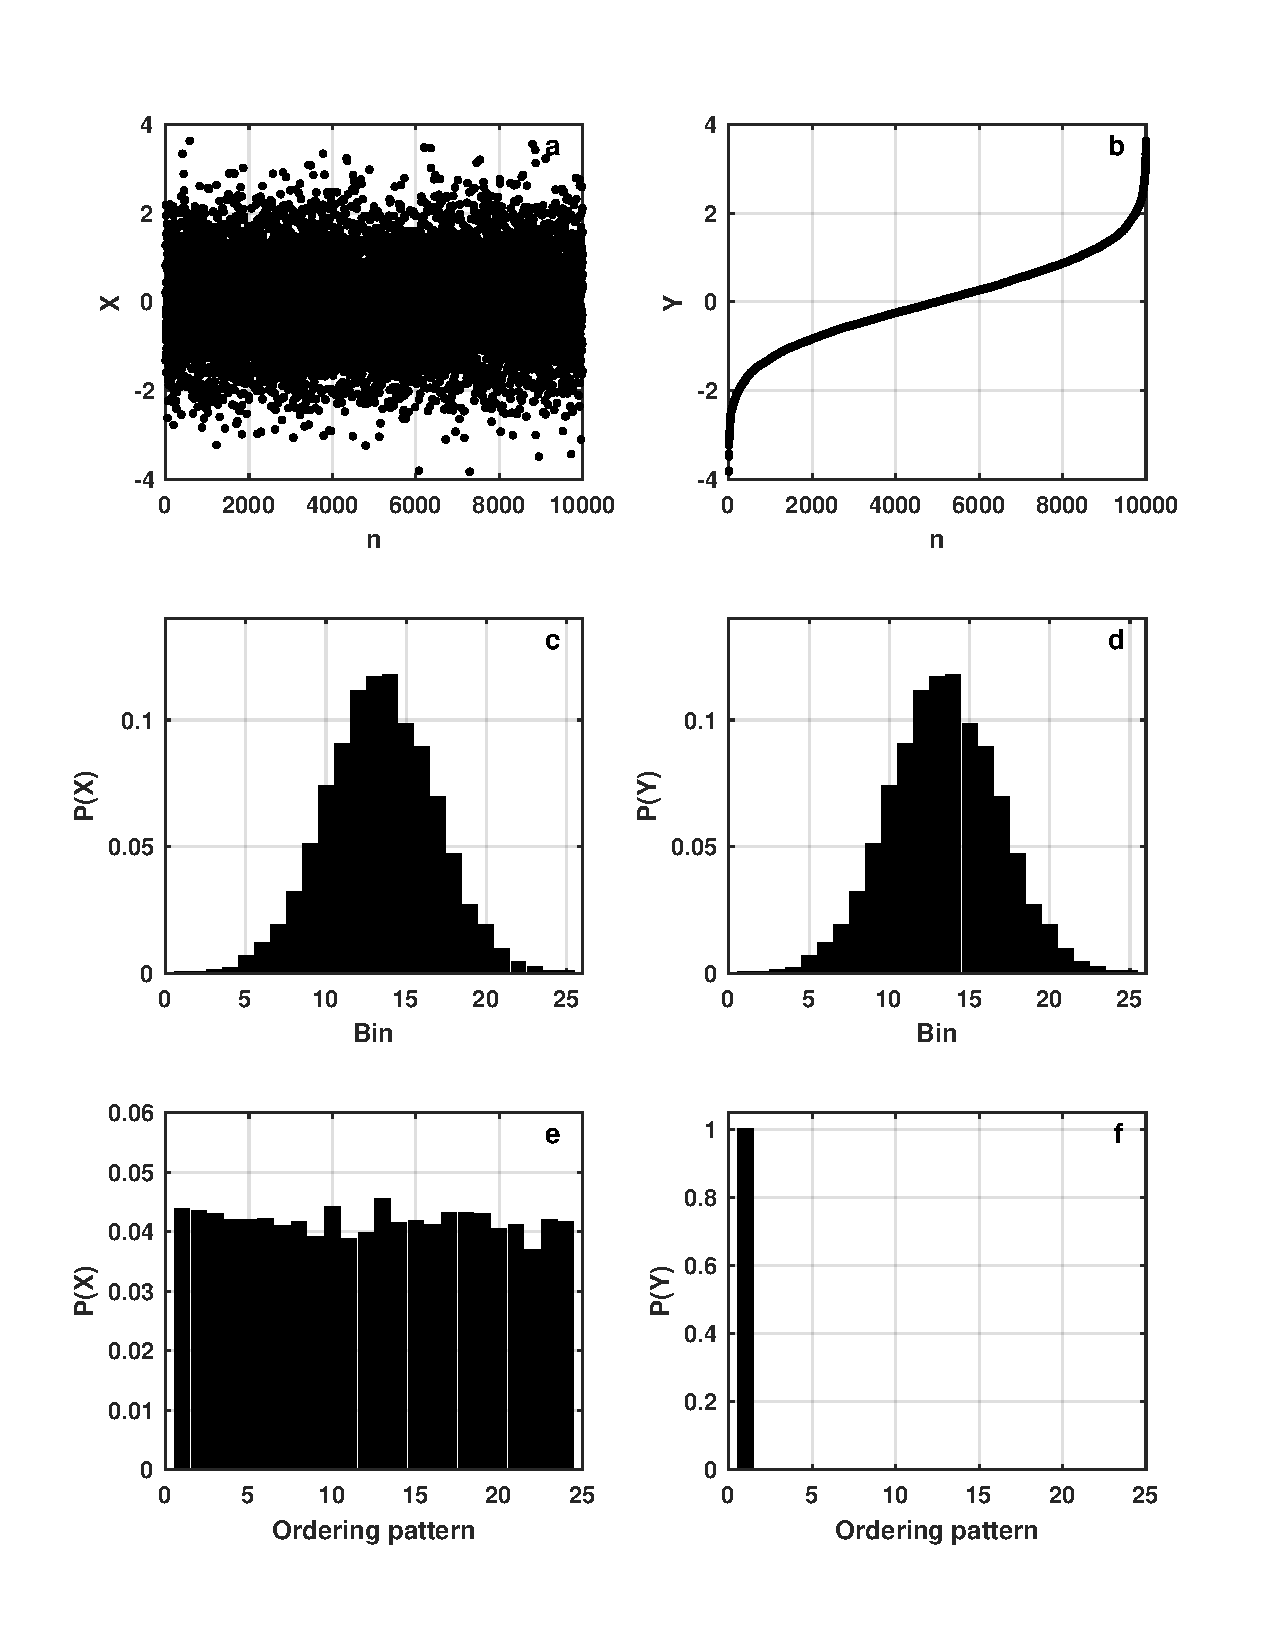
\includegraphics[width=1\textwidth]{causal_nocausal}
\caption{(see text) Time series $X$ obtained by using function \emph{randn} (a), its sorted version $Y$ (b) and their causal (c, d) and non-causal histograms (e, f).}
\label{fig:causal_nocausal}
\end{figure}

Let us consider now the case of sampled digital signals like as sampled \emph{RO}'s outputs are. Time series $X$ is binary and has a natural alphabet with two symbols
$\mathfrak{A}=\{0,1\}$. The Shannon entropy of this alphabet is usually known as \emph{Binary Entropy} $S_2$. Suppose $W$ consecutive bits of $X$ are grouped into \emph{a word}, that is the decimal number $w_i$ between $0$ and $2^W-1$; consider these decimal numbers as the symbols of the new alphabet and let $Z=\{w_i,~i=1,2,...\}$ be the new symbolic series. $S_W$ is the entropy of $P_{hist}(Z)$ where subscript \emph{hist} is for histogram; $S_W$ is also known as \emph{Block Entropy} of the binary time series $X$. Furthermore, if $D$ consecutive decimal numbers $w_i$ are grouped again and the $D!$ permutation patterns are considered as symbols of the new alphabet, we get a new $P_{BP}(Z)$, given by the relative frequencies of the permutation patterns. The entropy is $S^{(D)}_{BP}$, the \emph{Bandt \& Pompe entropy} \cite{Pompe2002} of the binary time series.
All the above-mentioned entropies are given by the same Shannon famous formula:
%
\begin{equation}
S~=~-~\sum_{j=1}^{m}{p_j~log(p_j)}, 
\end{equation}
%
and the only difference between them is the $P$ assigned to the time series. In this paper
$log$ means \emph{base $2$ logarithm}.

In this paper, we use a causal $P$ determined with the Bandt \& Pompe procedure. This procedure has been described in detail and successfully used in a number of papers concerning pseudo random number generation, system classifications, etc. \cite{Amigo2005,Rosso2007b,DeMicco2008,DeMicco2009,Amigo2010,Rosso2008}.
Let us summarize the basic procedure applied to our specific case:
\begin{itemize}
\item let $Z=\{w_i,~i=1,2,...\}$ be a numerical time series (in our case $W$ bits decimal numbers) series;
\item choose an embedding dimension $D~>~1$
\item assign to each $w_i$ a $D$-dimensional vector of previous $i, i-1,\cdots,i-(D-1)$:

\begin{equation}
\label{eq:vectores}
(s)\mapsto \left(w_{i-(D-1)},w_{i-(D-2)},\cdots,w_{i-1},w_{i}\right)
\end{equation}

Clearly, the greater the $D-$value, the more information about ``the past" is incorporated into these vectors. 
\item look for \emph{ordinal patterns} of length $D$ \cite{Pompe2002,Keller2003,Keller2005}. By ``ordinal pattern" related to position $i$ we mean the permutation $\pi=(r_0, r_1, \cdots,r_{D-1})$ of $(0, 1, \cdots, D-1)$ defined by

\begin{equation}
\label{eq:permuta}
w_{i-r_{D-1}}\le w_{i-r_{D-2}}\le\cdots\le w_{i-r_{1}}\le a_{i-r_0}
\end{equation}
\item In order to get a unique result consider that $r_j <r_{j-1}$ if $x_{i-r_{j}}=x_{i-r_{j-1}}$. 
\item Thus for all the $D!$ possible permutations $\pi$ of order $D$ is the probability distribution $P=\{p(\pi)\}$ defined by

\begin{equation}
\label{eq:frequ}
p(\pi)~=~ \frac{\sharp \{s|s\leq M-D+1; i \quad \texttt{has type}~\pi\}}{M-D+1}
\end{equation}

In the last expression, the symbol $\sharp$ stands for ``number" and corresponds to the number assigned to the permutation using the lexicographic order . 
\end{itemize}

The main advantages of the Bandt \&Pompe method are {\it a)\/} its simplicity, {\it b)\/} the extremely fast nature of the pertinent calculation-process, {\it c)\/} its robustness in the presence of observational and dynamical noise, and {\it d)\/} its invariance with respect to nonlinear monotonous transformations. The Bandt \&Pompe methodology is not restricted to time series representative of low dimensional dynamical systems but can be applied to any type of time series (regular, chaotic, noisy, or reality based), with a very weak stationary assumption (for $k~=~D$, the probability for $a_i < a_{i+k}$ should not depend on $i$ \cite{Pompe2002}).

Let us stress some important issues involved in the calculations of the above-mentioned entropies:
\begin{enumerate}
\item The binary entropy $S_2$ is noncasual while both, the block entropy $S_W$ and the Bandt \& Pompe entropy $S^{(D)}_{BP}$, are causal. 
\item The block entropy $S_W$ takes into account correlations between $W$ consecutive bits. Bandt\& Pompe entropy $S^{(D)}_{BP}$ takes into account correlations between $D$ consecutive $W$-length words.
Both grouping procedures (decimal numbers of $W$ bits and permutation patterns of $D$ decimal numbers) may be done with or without superposition. The number of data required for good statistics is different depending the grouping procedures are made with superposition or not.
\item For $S_W$ there is only one grouping process ($W$ bits are grouped to obtain a decimal numbers time series $Y$). Let us define $\alpha$ as a statistical quality parameter, given by the quotient between the number of elements in the symbolic time series $Y$ and the number of symbols in the alphabet. In this paper we will not accept $\alpha~<~10$. 

Obviously the quality factor $\alpha$ increases with the length of the time series:
%
\begin{enumerate}
\item If the grouping of $W$ bits is made with superposition, two consecutive $W$-length words share $W-2$ bits. Consequently starting with a file with a length of $N$-bits we get $N-W+1$ words. Furthermore, there are $2^W$ symbols in the alphabet and $\alpha=(N-W+1)/(2^W)$. 
\item If $S_W$ is evaluated without superposition the number of $W$-length words is $floor~\{N/W\}$ and the quality parameter becomes $\alpha=floor~\{N/W\}/(2^W)$. For $N\gg W$ the statistical quality factor is $W$ times lower that the one with superposition.
\end{enumerate}

\item In the case of $S^{(D)}_{BP}$, there are two grouping processes involved. 
\begin{enumerate}
\item If both grouping processes are made with superposition we get $N-W-D+2$ elements starting with a file $N$-bits length, and the quality factor is $\alpha=(N-W-D+2)/D!)$. In this case $S^{(D)}_{BP}$ takes into account the correlations between $W+D$ consecutive bits. 
\item If the grouping process of $W$ bits is made without superposition but the grouping of $D$ decimal numbers is made with superposition we get $floor\{N/W\}-D+1$ elements and the statistical quality parameter is $\alpha=(floor\{N/W\}-D+1)/D!$. In this case $S^{(D)}_{BP}$ will include correlations between $WD$ consecutive bits. 
\item If the grouping process of $W$ bits is made with superposition and the grouping of $D$ decimal numbers is made without superposition we get $floor\{(N-W+1)/D\}$ elements starting from a file with $N$ bits.The statistical quality factor is $\alpha=floor\{(N-W+1)/D\}/D!$ and $S^{(D)}_{BP}$ takes into account correlations between $W+D-1$ bits.
\item If both grouping processes are made without superposition we get $floor\{floor\{N/W\}/D\}$ elements starting from a $N$-bits length file. The statistical quality factor is $\alpha=floor\{floor\{N/W\}/D\}/D!$ and $S^{(D)}_{BP}$ takes into account correlations between $WD$ consecutive bits.
\end{enumerate}
\end{enumerate} 

\subsubsection{Additional quantifiers}
\label{subsec:addquanti}

The Shannon Entropy $S(P)$ is the startpoint for other quantifiers:
\begin{enumerate}
\item Normalized entropy $H(P)$: it is the Shannon Entropy divided by its maximum value. For example, if we use $S_2$ (see above), the maximum entropy is obtained for equiprobability between two symbols. Its value is $S_{max}=-1/2 log(1/2)-1/2 log(1/2)=log(2)=1$; then, the normalized entropy is $H_2=S_2$. If we use $S_W$ the equiprobability between the $2^W$ possible words ($W$-bits decimal numbers) produces $S_{max}=W$ and $H_W=S_W/W$. Finally for $S^{(D)}_{BP}$ the equiprobability between the $D!$ ordinal patterns produces $S_{max}= log(D!)$ and $H^{(D)}_{BP}=S^D_{BP}/log(D!)$.
\item Differential or conditional entropies $h$ and $h^*$ are:
\begin{eqnarray}
h~=~S_{W+1}-S_W\\
h^*~=~S_{BP}^{(D+1)}-S_{BP}^{(D)}
\end{eqnarray}
In the above expressions $W=1,2,...$ and $D=2,3,...$, $S_0=0$ and $S_{BP}^{(1)}=0$. These differential or conditional entropies give the average amount of information required to predict the $(W+1)$ (or $(D+1)$) symbol, given the preceding $W$ (or $D$) symbols.
\item Finally the \emph{rate entropies} $h_0$ and $h_0^*$ are given by:

\begin{eqnarray}
h_0=\lim\limits_{W\rightarrow \infty} h=\lim\limits_{W\rightarrow \infty}{S_{W}/W }\\
h^*_0= \lim\limits_{D\rightarrow \infty} h^*=\lim\limits_{D\rightarrow \infty}{S^{(D)}_{BP}/(D-1)}
\end{eqnarray}

\end{enumerate}

Let us tell in advance that we shall show in section \ref{sec:resu} that quantifiers $S_W$, $S^{(D)}_{BP}$ , $H_W$ and $H^{(D)}_{BP}$ are dependent on parameters $W$ and $D$. This is a drawback if we want to use them as jitter measures. On the other hand, the estimators $h$ and $h^*$ of the \emph{rate entropies} $h_0$ and $h^*_0$ \cite{Ebeling2001,Amigo2005} instead, are independent of $W$ and $D$ and we will show in Section \ref{sec:resu} that in the case of sampled \emph{RO}'s they also present a minimum for the correct sampling ratio making them good measure of the quality of both \emph{RO}'s and \emph{PRNG}'s derived from them. 

\subsection{Results}
\label{sec:resu}

An evenly sampled output of a jitter-less \emph{RO} was simulated with Matlab\textsuperscript{\copyright} and an output file with a length of $N_b=7,000,000$ of bits was generated. A set of a hundred values of the sampling ratio $r= T_s/T\in[6.5,9.5]$, was explored (where $T_s$ is the sampling period and $T$ is the \emph{RO}  output period). Jitter with a normal distribution and a set with different values of variance $\sigma_s$ (see below) were added to the original file. Our method emulates the real process of sampling the noisy output of a real \emph{RO}; the detailed code is published in Mathworks\cite{MathworksMaxi}.

For each value of $\sigma_s$, ten surrogates (each one with a different random initial condition) were generated and new files with $N_b$ bits each were stored. It was assumed that jitter of individual samples is independent, normal distributed random variables, with zero mean value and variance $\sigma_i=\sigma_s$. Consequently, the variance of the accumulated jitter over one period $T$ is given by $\sigma^2_T=r \sigma^2_s$ \cite{Valtchanov2008}. The values considered  are $\sigma_T=\{0,$ $0.001,$ $0.002,$ $0.003,$ $0.004,$ $0.005,$ $0.007,$ $0.01,$ $0.02,$ $0.02,$ $0.04,$ $0.05,$ $0.07,$ $0.1\}$.

For each file all the quantifiers defined in \ref{sec:quanti} were evaluated for $D\in[2,10]$ and $W\in[1,26]$. The details about evaluation, advantages and drawbacks of each quantifier are reported in section \ref{sec:quanti}: they are $S_W$, $S^{(D)}_{BP}$, $H_{W}$, $H^{(D)}_{BP}$, $h$ and $h^*$.  Let us only show here the  more relevant results  to show the reason the last two quantifiers ($h$ and $h^*$) are the best ones.

\begin{itemize}
\item In the case of normalized entropy $H_{W}$, it strongly depends on $W$. Furthermore the analysis of $H_{W}$ as a function of $r$ shows that it does not allow to determine an optimum value of the sampling ratio $r$ (see Fig. \ref{fig:H_W_rCS}). This is an important issue if the quantifiers are going to be used for experimental setups. 
\item In the case of the normalized Bandt \& Pompe entropy $H^{(D)}_{BP}$, a strong dependence on the embedding dimension $D$ is additionally present. Again it is not easy to determine the optimum value of $r$ from the analysis of this parameter as a function of $r$  (see Fig. \ref{fig:HBP_W_rSS}). 
\item A similar behavior appears in all the other functionals related with these two entropies. 
In summary, our results show that  both $ h$ y $h^*$ are independent of any arbitrary parameter used in their statistical determination.  These two quantifiers have also been considered in two excellent articles \cite{Amigo2006,Ebeling2001}. 
\end{itemize}
%
\begin{figure}
\center
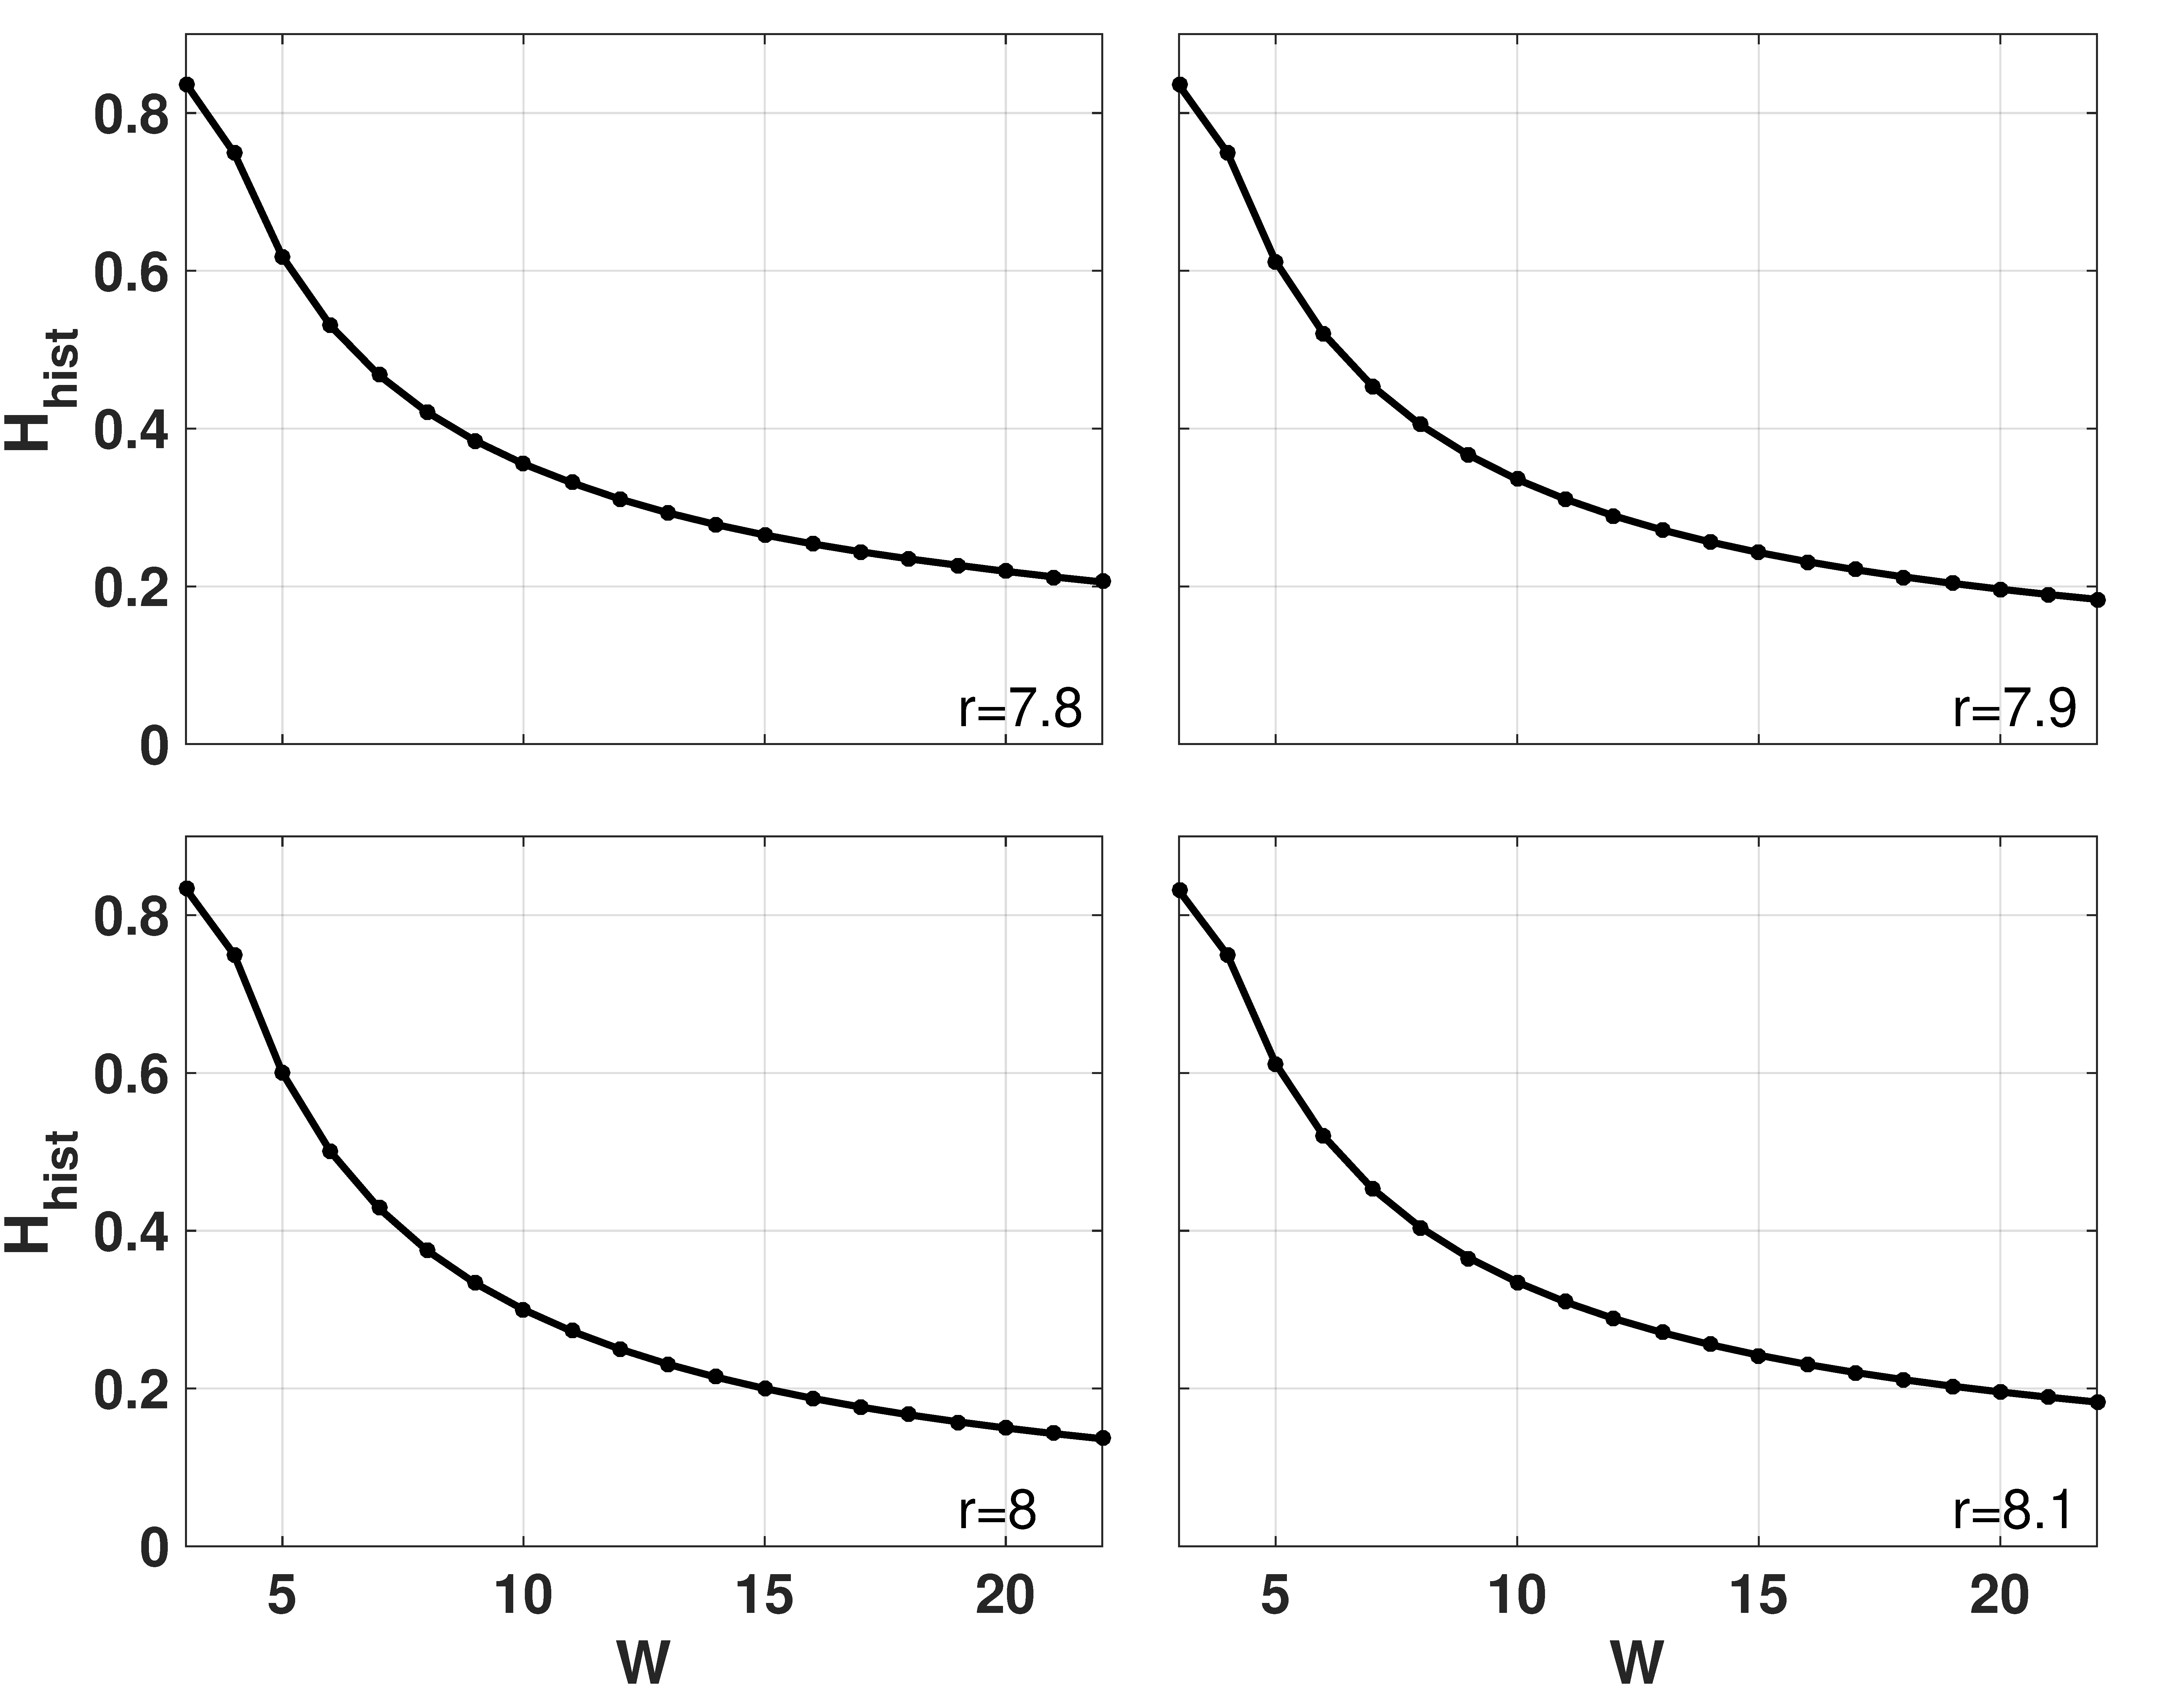
\includegraphics[width=0.8\textwidth]{H_W_rCS}
\caption{Normalized entropy $H_W$ as a function of $W$ for a jitter-less \emph{RO} sampled with different values of $r$.}
\label{fig:H_W_rCS}
\end{figure}
%
\begin{figure}
\center
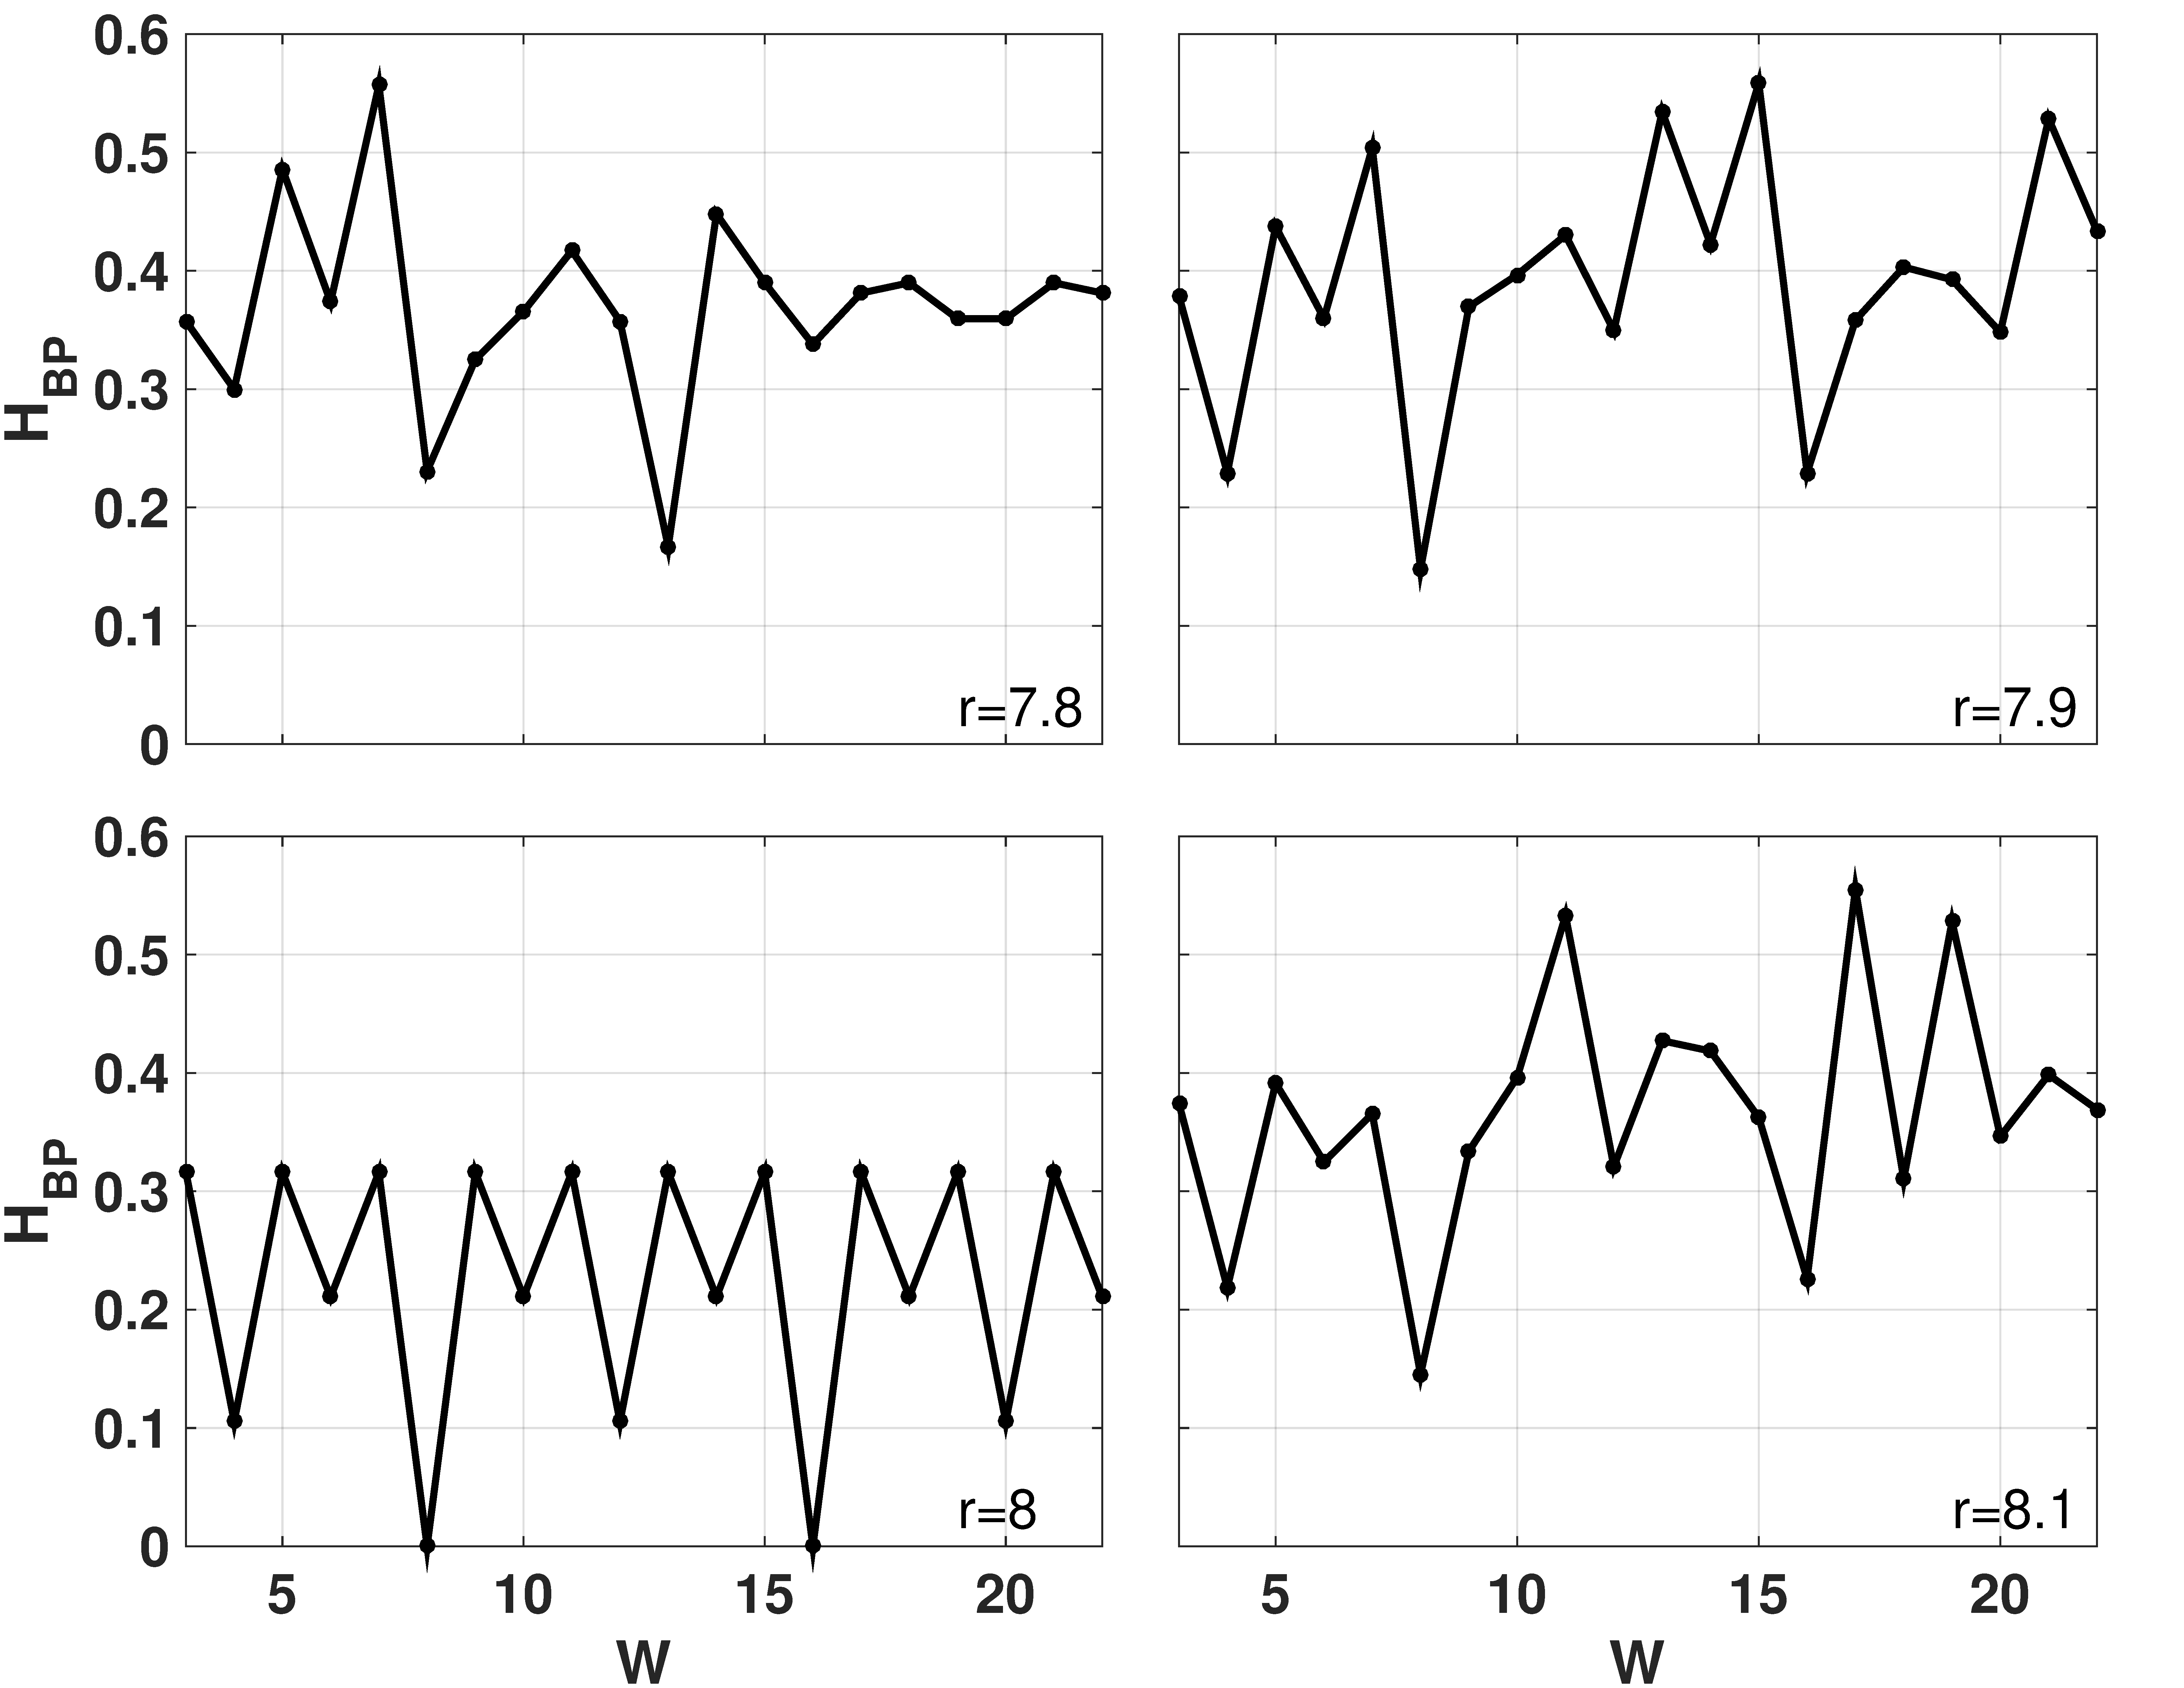
\includegraphics[ width=0.8\textwidth]{HBP_W_rSS}
\caption{$H^{(D)}_{BP}$ as a function of $W$ for a jitter-less \emph{RO} sampled with different values of $r$. Calculations are made without superposition of words}
\label{fig:HBP_W_rSS}
\end{figure}

Our results show that two quantifiers, $h$ and $h^*$, are appropriate to be used as jitter measures because: 
\begin{itemize} 
\item (a) for $\sigma_T=0$ (jitter-less output) they rapidly approach to a constant limiting value as both $D$ and $W$ increase toward $\infty$ and this limiting value is independent of both $D$ and $W$; 
\item (b) they are increasing monotone (and almost proportional) functions of $\sigma_T$. \item (c) From their analysis, it is possible to detect the optimum value of the sampling ratio $r$. Let us show these claims in the following figures that are representative of all our results. 
\end{itemize}
%
Figure \ref{fig:hm_D_SJ} shows the Bandt \& Pompe differential entropy $h^*$, as a function of $D$, with $W$ as a parameter, for a ring without jitter. It can be seen that there is a threshold value $W=4$ over which all the curves collapse into one for every value of $D$. Furthermore, Fig. \ref{fig:hm_D_SJ} also shows that for $D\ge8$ all the curves collapse into one, regardless the value of $W$. In conclusion, if $D\ge 8$ and $W\ge 4$ one obtains a quantifier independent of both $D$ and $W$. The influence of jitter on this quantifier is shown in Figure \ref{fig:hm_D_CJ}, where $h^*$ is plotted as a function of $D$ with $\sigma_T$ as a parameter. The values considered are $\sigma_T=\{0 (no~jitter),$ $0.001,$ $0.002,$ $0.003,$ $0.004,$ $0.005,$ $0.007,$ $0.01,$ $0.02,$ $0.02,$ $0.04,$ $0.05,$ $0.07,$ $0.1\}$. The inset of Fig. \ref{fig:hm_D_CJ} shows $h^*$ as a function of $\sigma_T$ for $D=8$. This inset shows that this quantifier is an increasing monotone function of $\sigma_T$. Finally Fig. \ref{fig:hm_r_CJ} shows $h^*$ as a function of the sampling ratio $r$. 
In this figure, it is shown that there is a minimum for the right $r$ (in this case $r=8$). Furthermore sensitivity of $h^*$ as a function of jitter is maximum for this same ideal value of $r$.

\begin{figure}
\center
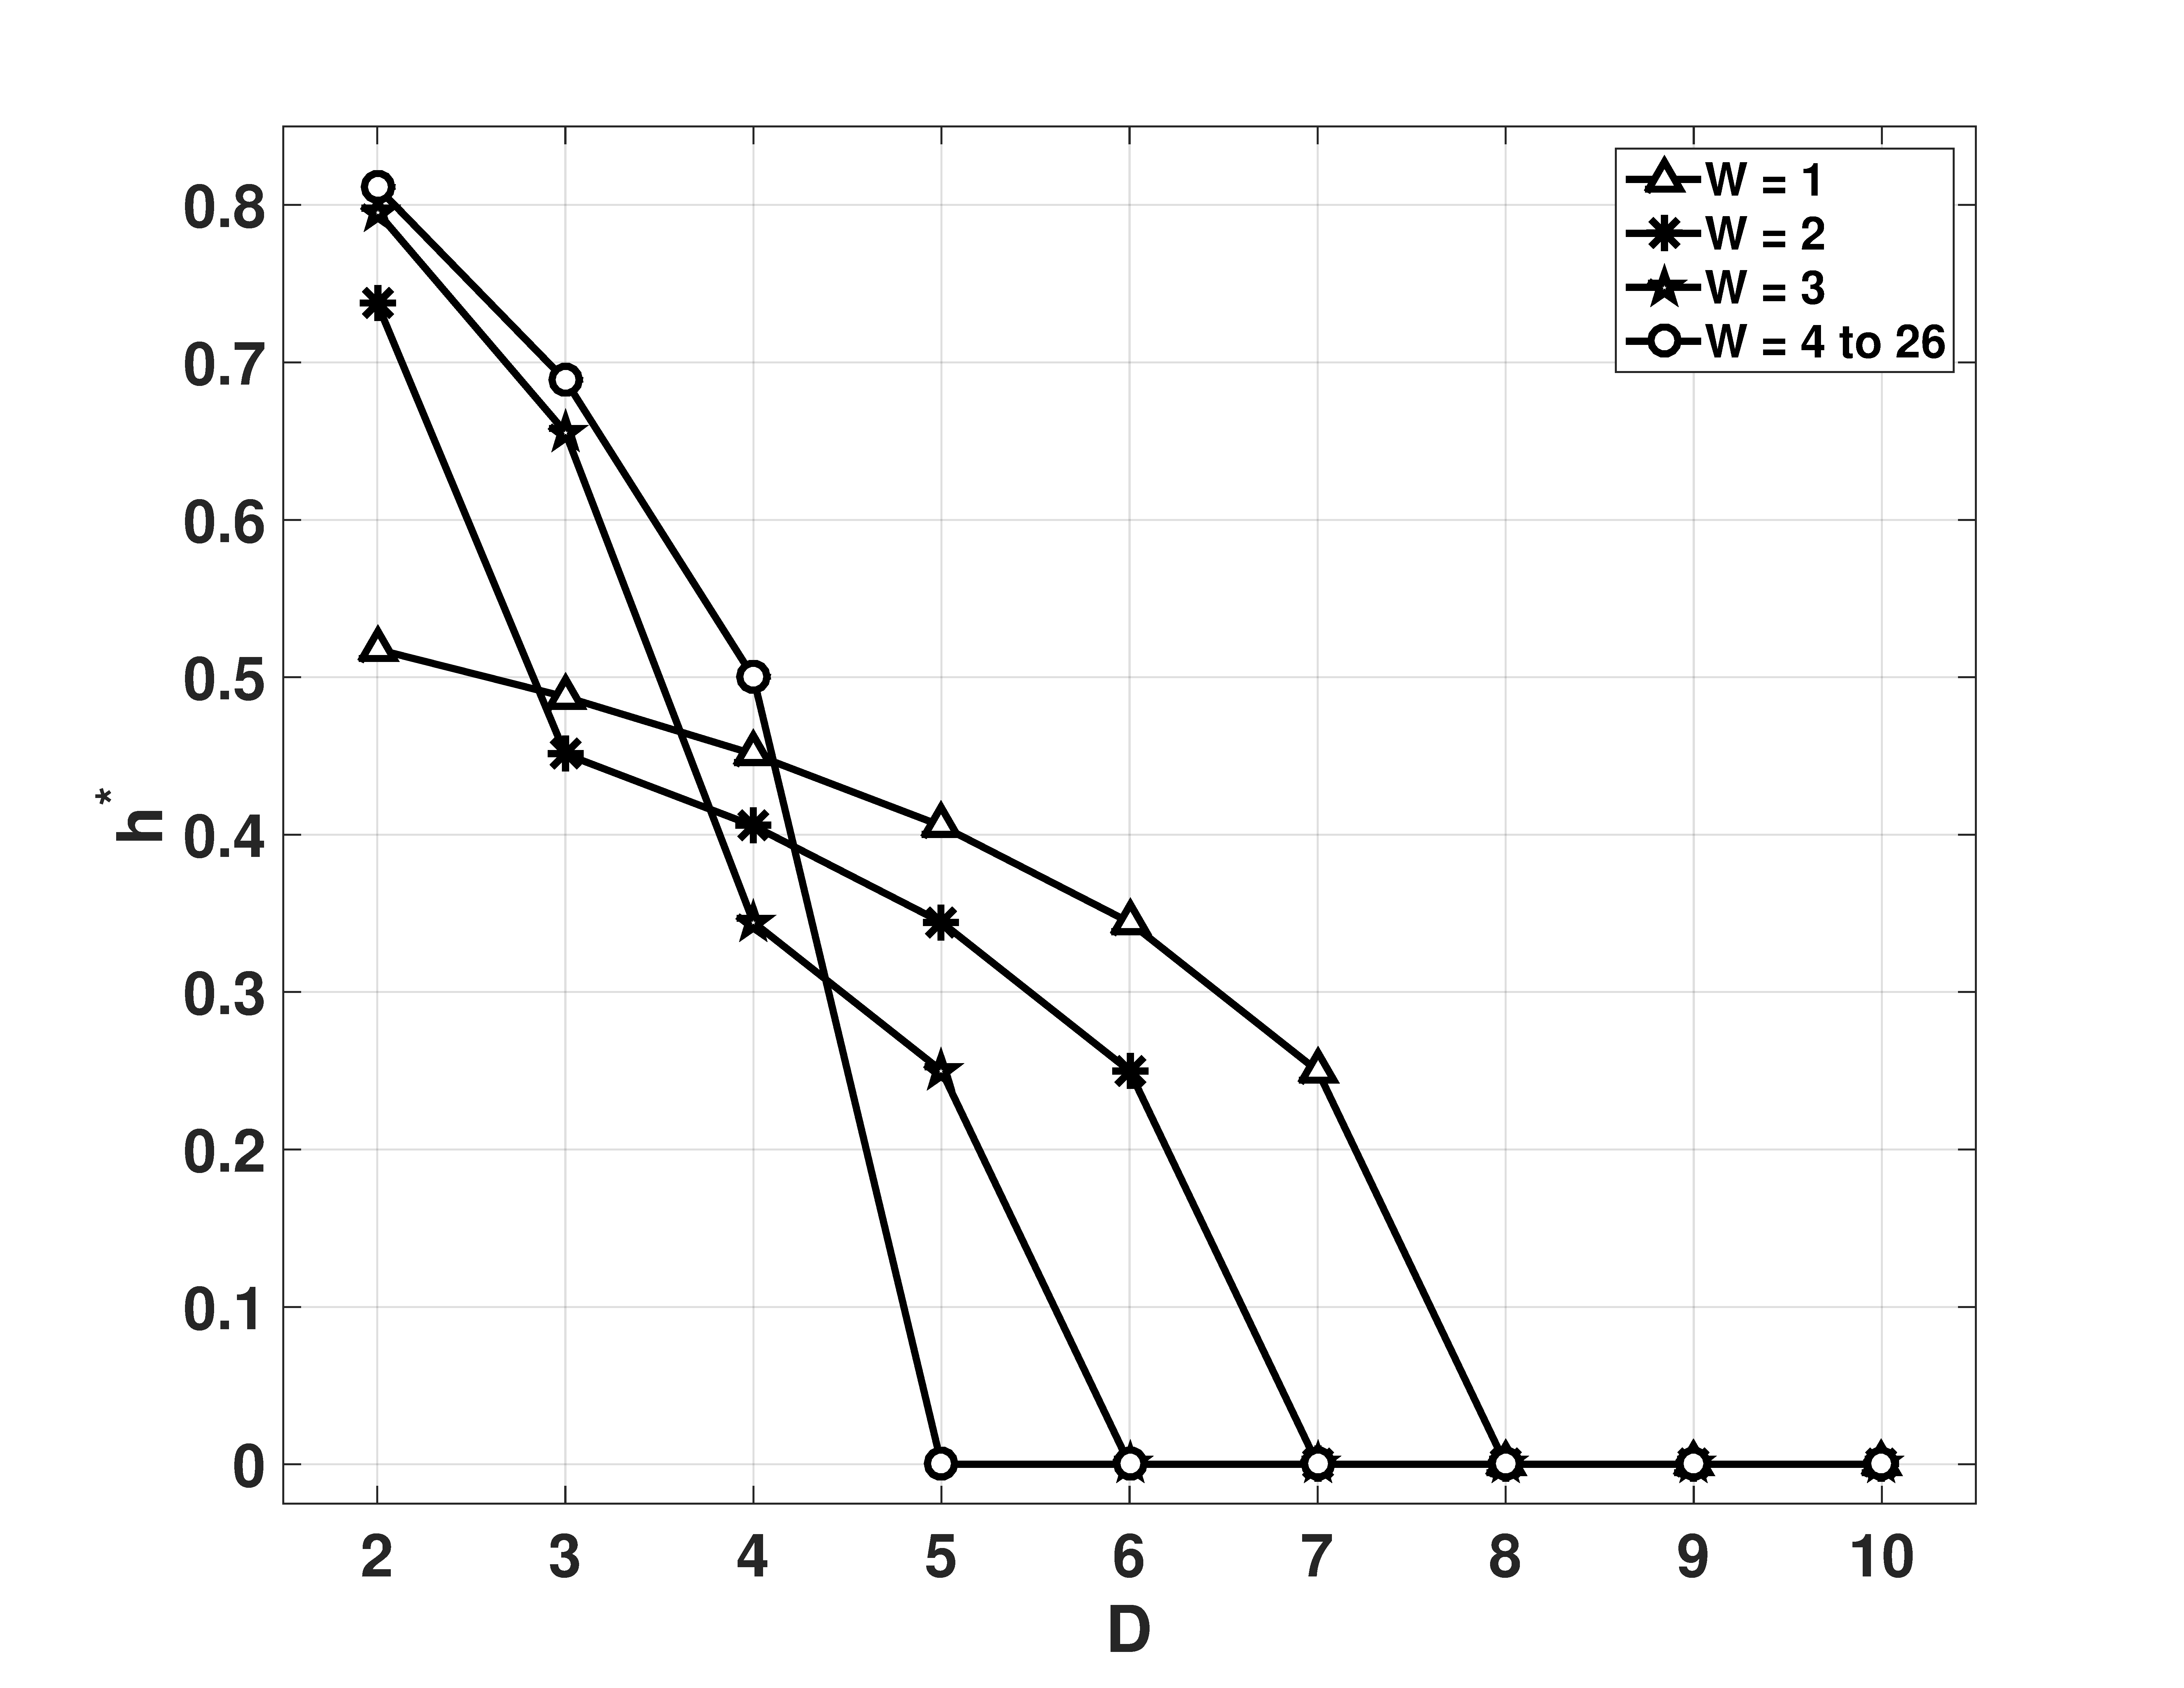
\includegraphics[ width=0.8\textwidth]{hm_D_SJ}
\caption{$h^*$ as a function of $D$ for a jitter-less \emph{RO} sampled with $r=8$.}
\label{fig:hm_D_SJ}
\end{figure}

\begin{figure}
\center
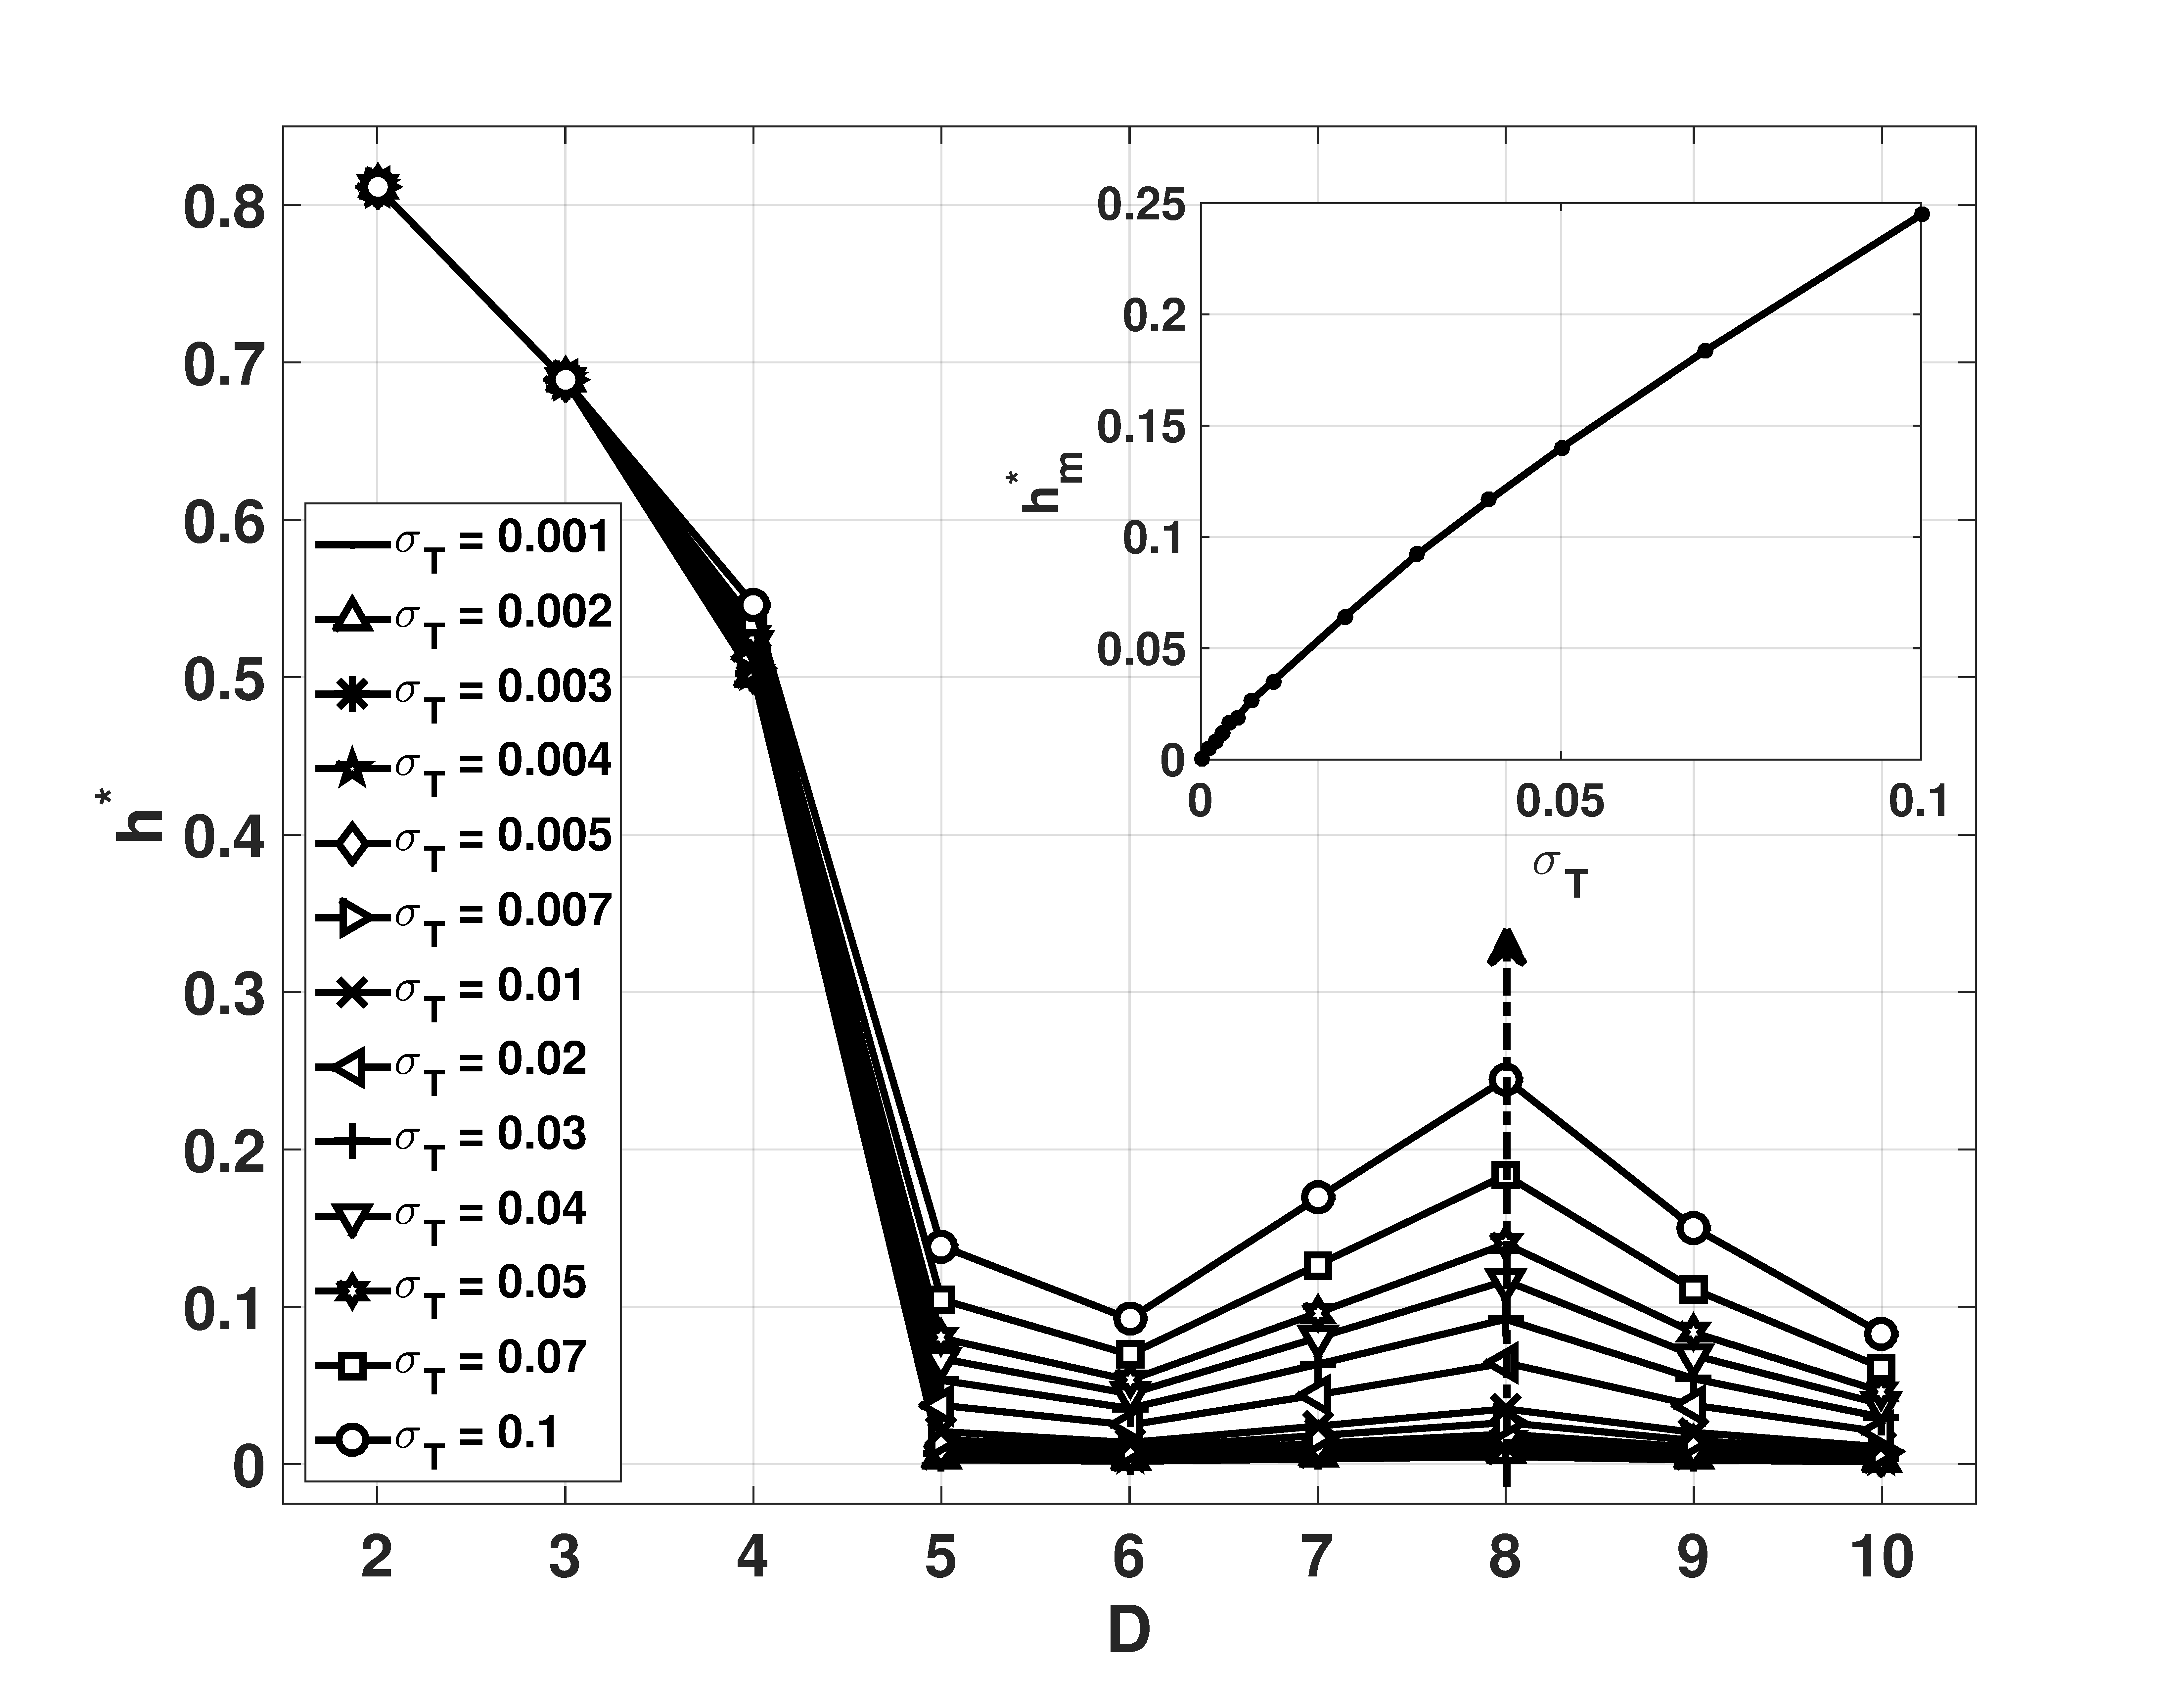
\includegraphics[width=0.8\textwidth]{hm_D_CJ}
\caption{$h^*$ as a function of $D$ for a \emph{RO} sampled with $r=8$ for a world length $W=6$ for jitter with several variances. The inset shows $h^*$ as a function of $\sigma_T$ for $r=8$, $W=6$ and $D=8$.}
\label{fig:hm_D_CJ}
\end{figure}

\begin{figure}
\center
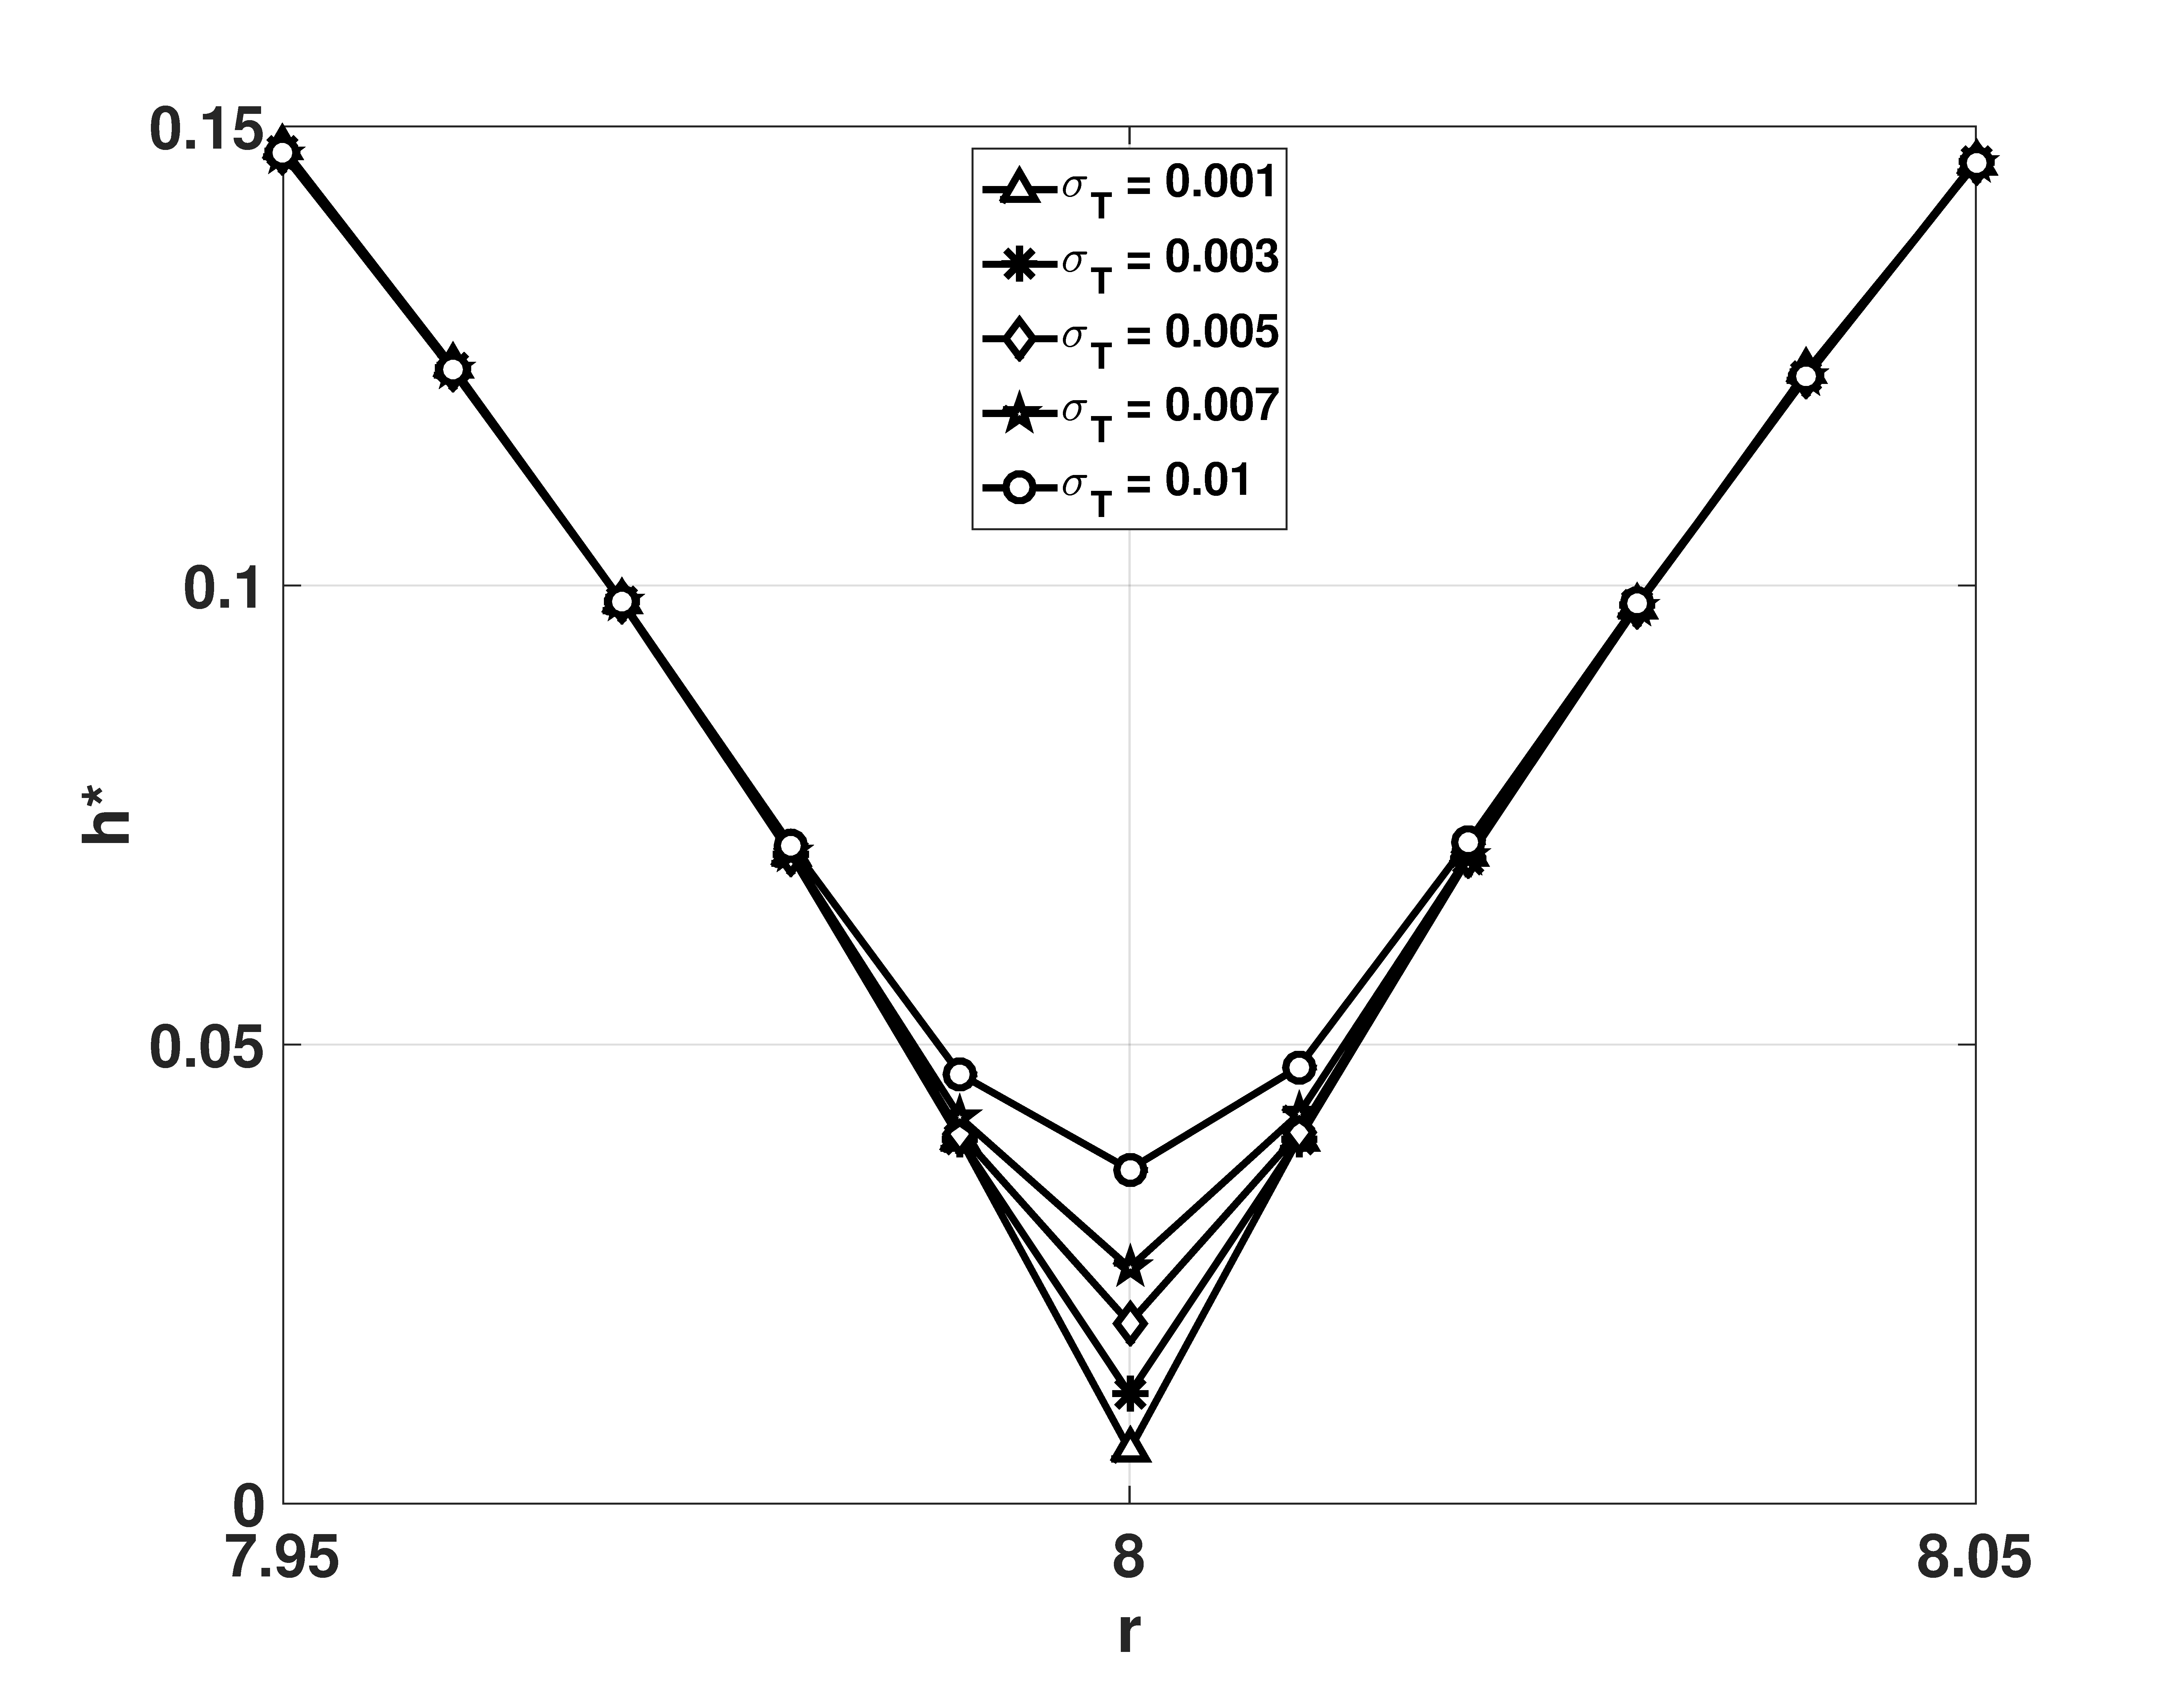
\includegraphics[ width=0.8\textwidth]{hm_r_CJ}
\caption{$h^*$ as a function of $r$ for $r\in[7.95,8.05]$, with several $\sigma_T$, $W=6$ and $D=8$. The curve has a minimum at the correct value $r=8$.}
\label{fig:hm_r_CJ}
\end{figure}

Let us now analyze the second quantifier, $h$. This quantifier only depends on $W$ because $D$ is not used to define the \emph{PDF} assigned to the data series. Fig. \ref{fig:h_W_SJ} shows jitter-less case, $h$ is almost independent of $W$ for $W\ge4$. In this paper, we adopted $W=6$. Figure \ref{fig:h_W_CJ} shows the influence of jitter over this quantifier. It is clear from the inset in this figure that, for the selected value $W=6$, $h$ is an increasing monotone function of jitter variance $\sigma_T$.

Fig. \ref{fig:h_r_CJ} shows that $h$ has a minimum when the value of $r$ takes its optimum value ($r=8$). Note that this minimum is robust also in the presence of jitter.

\begin{figure}
\center
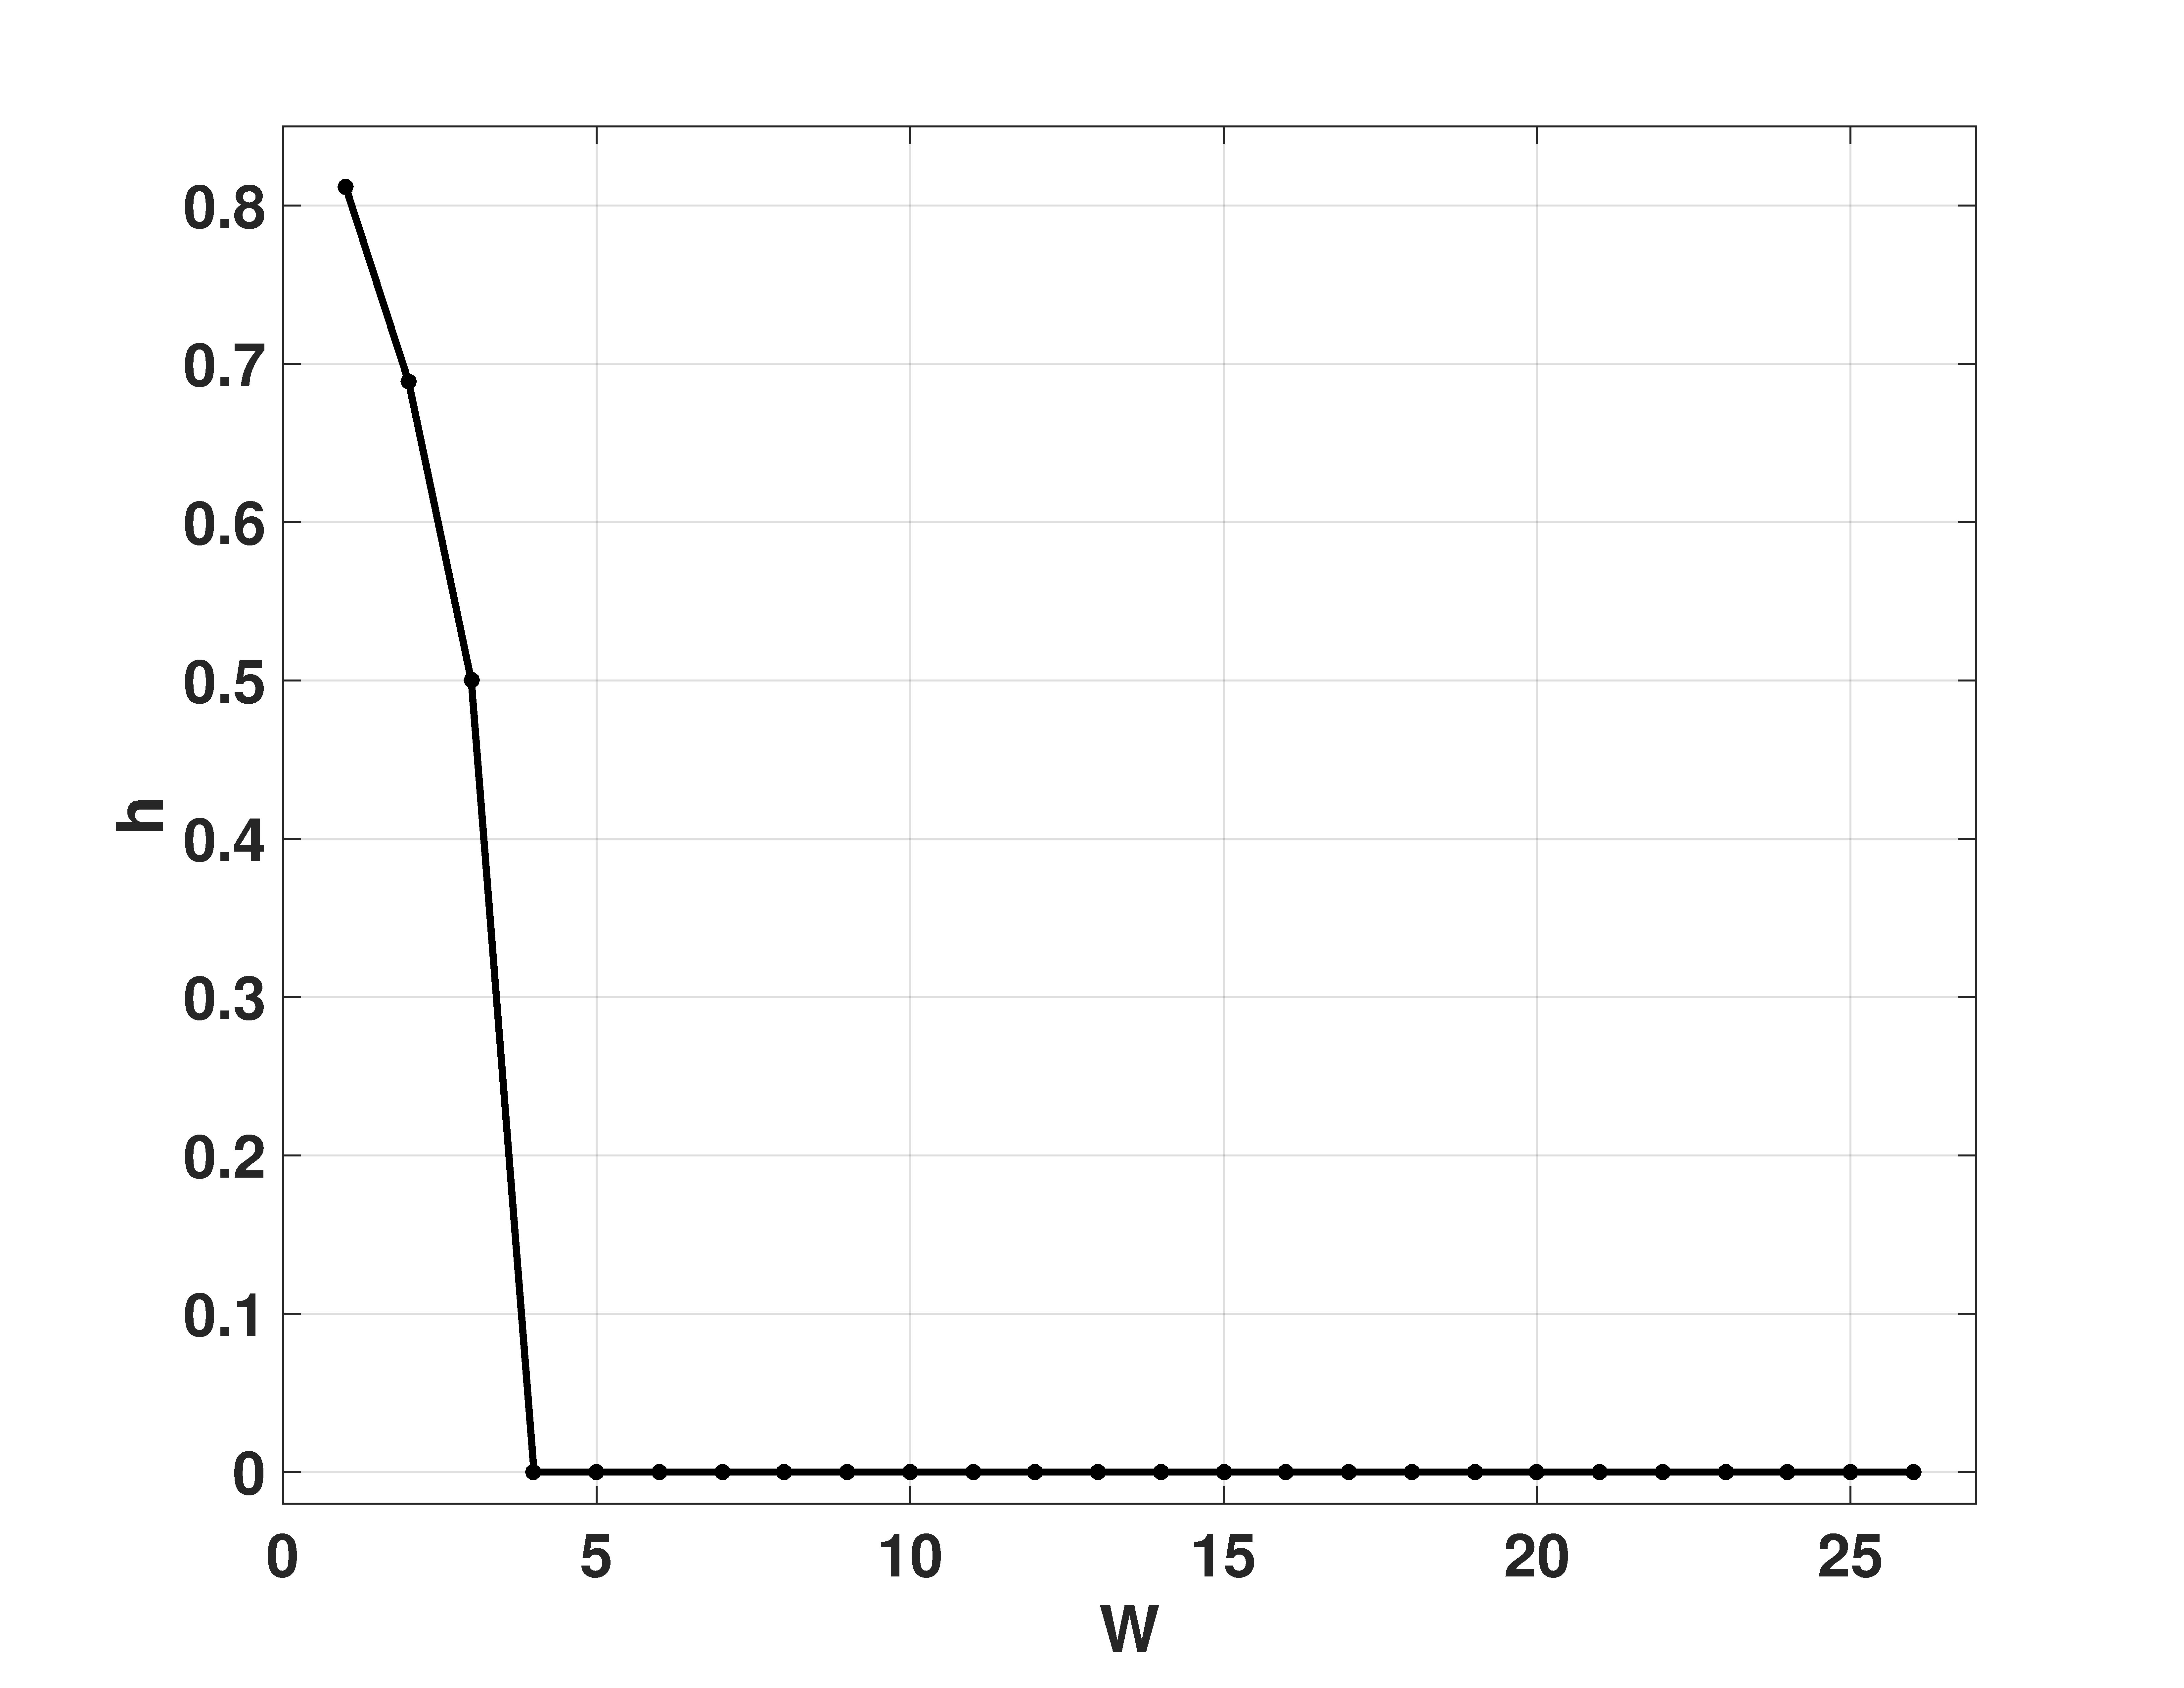
\includegraphics[width=0.8\textwidth]{h_W_SJ}
\caption{$h$ as a function of $W$ for a jitter-less \emph{RO} sampled with $r=8$.}
\label{fig:h_W_SJ}
\end{figure}

\begin{figure}
\center
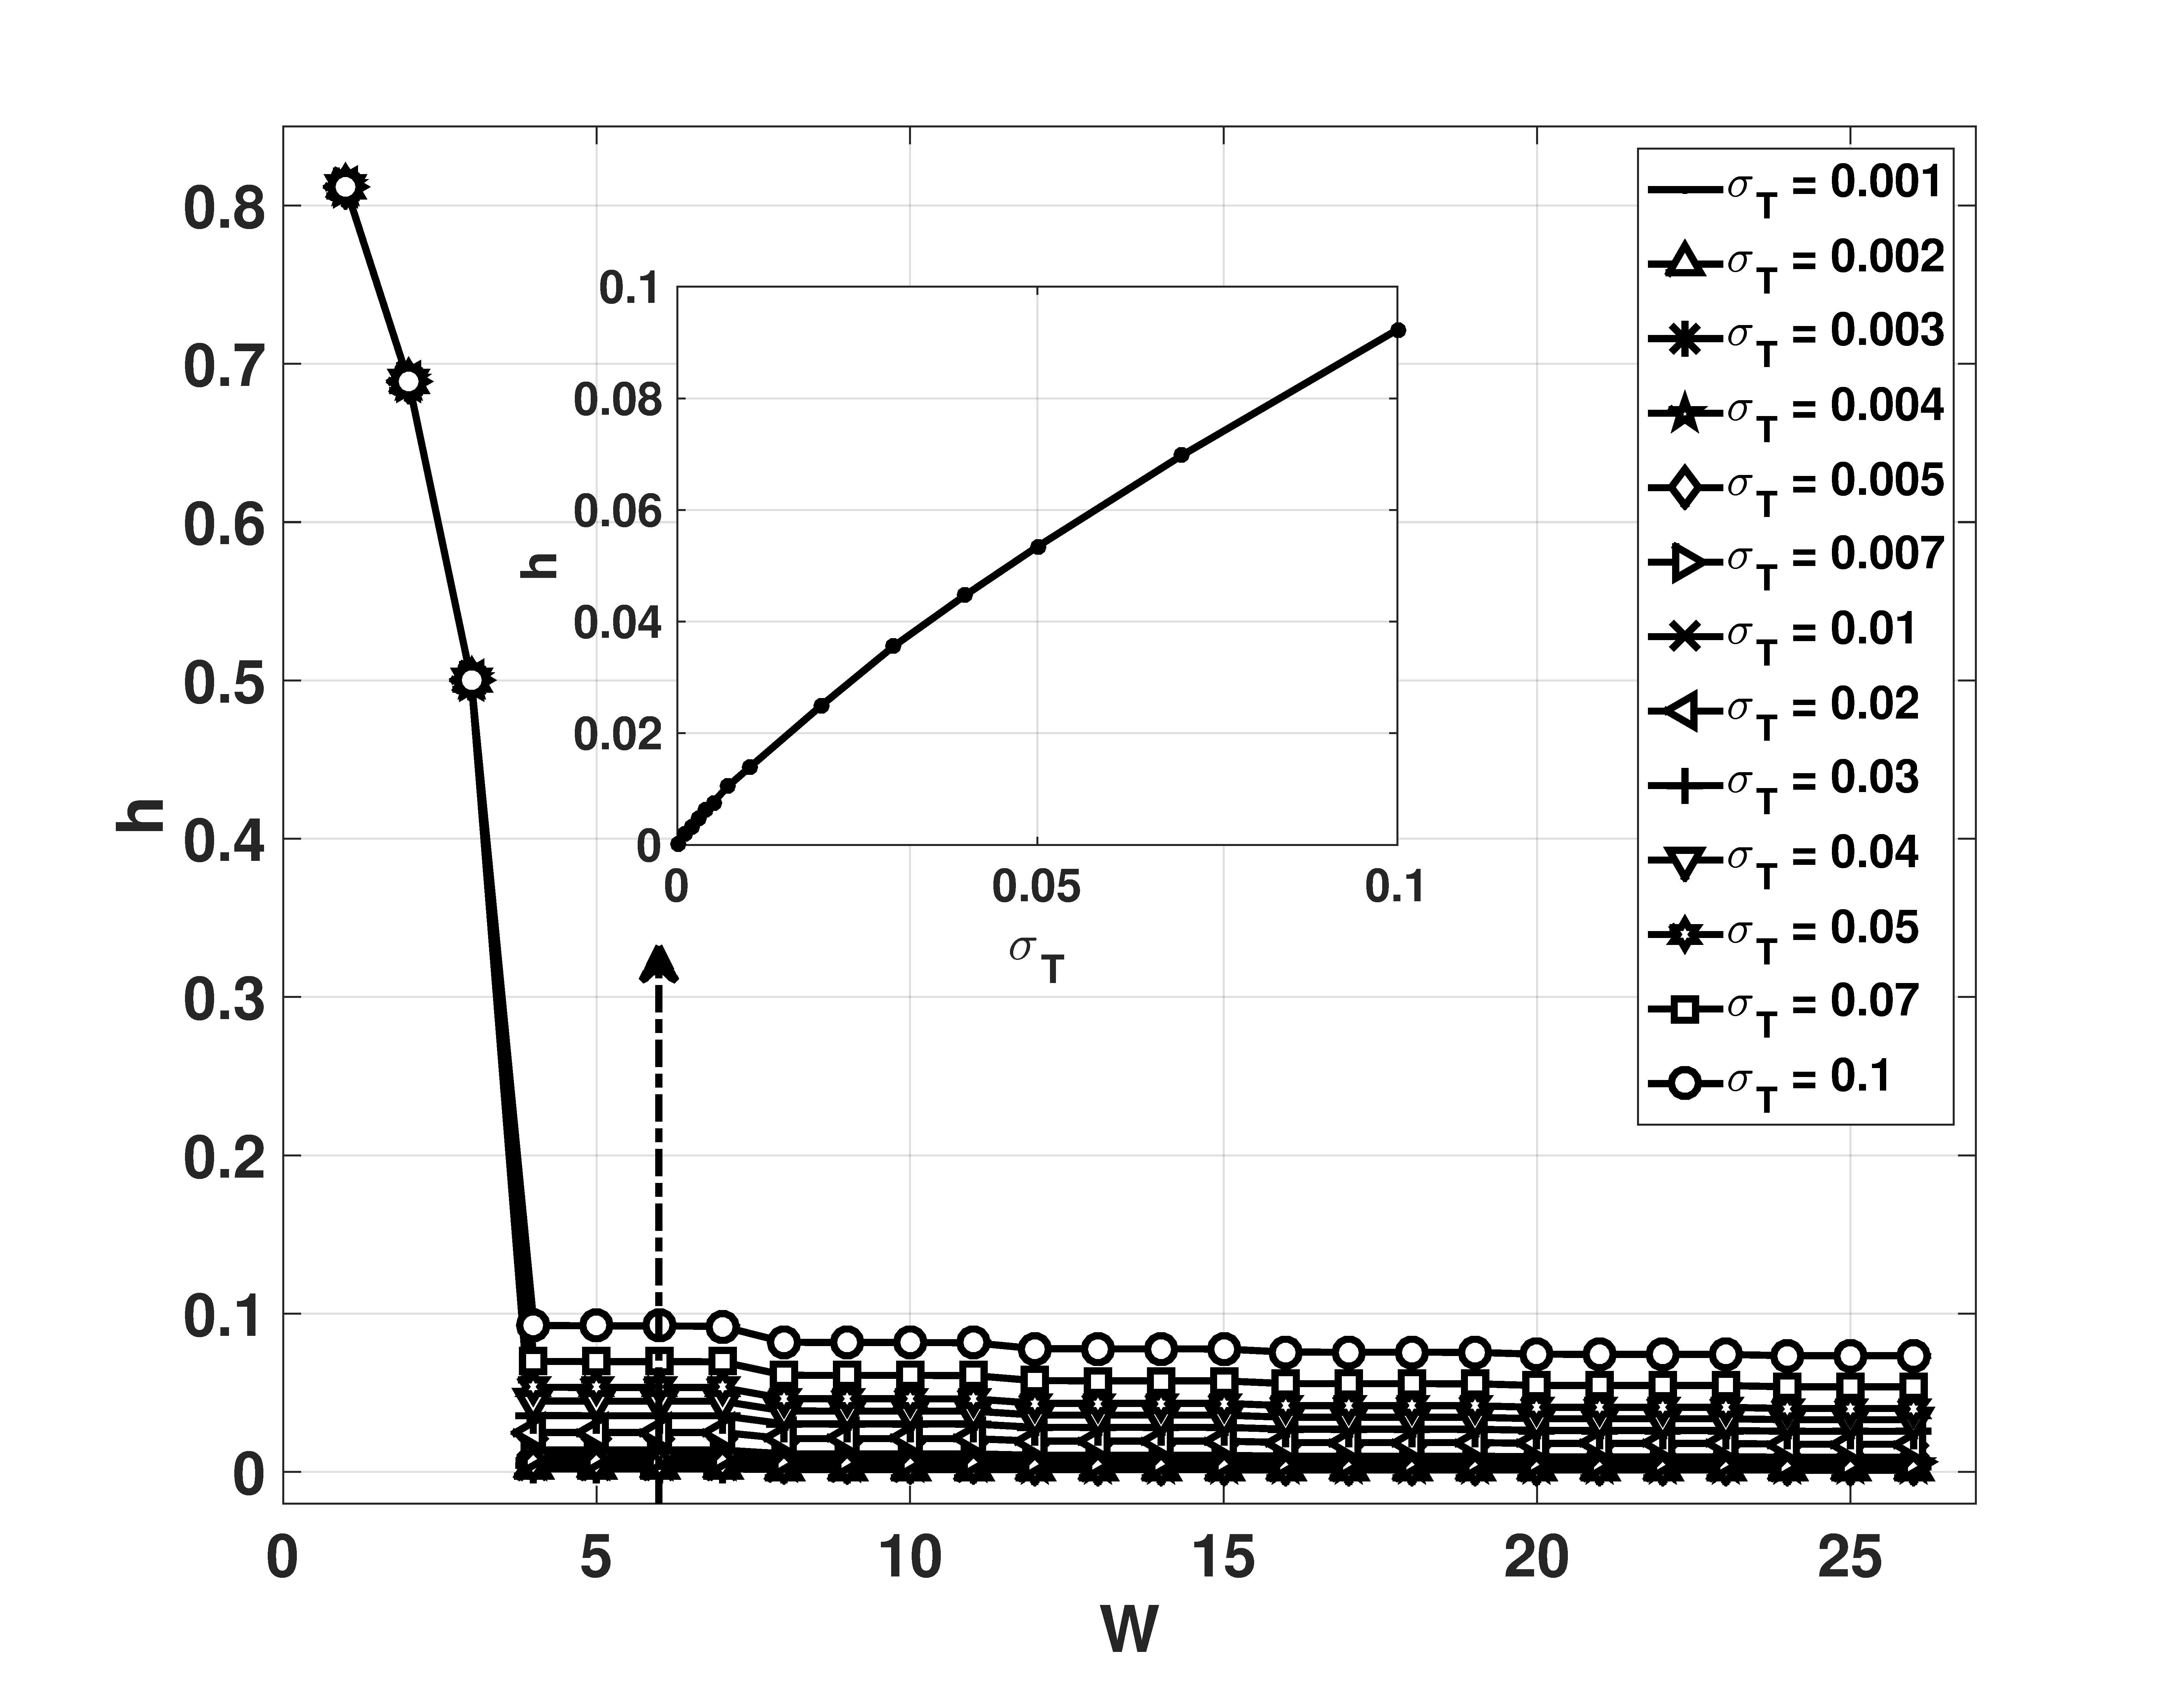
\includegraphics[ width=0.8\textwidth]{h_W_CJ}
\caption{$h$ as a function of $W$ for a \emph{RO} sampled with $r=8$, for jitter with several variances. The inset shows $h$ as a function of $\sigma_T$ for $r=8$ and $W=6$.}
\label{fig:h_W_CJ}
\end{figure}

\begin{figure}
\center
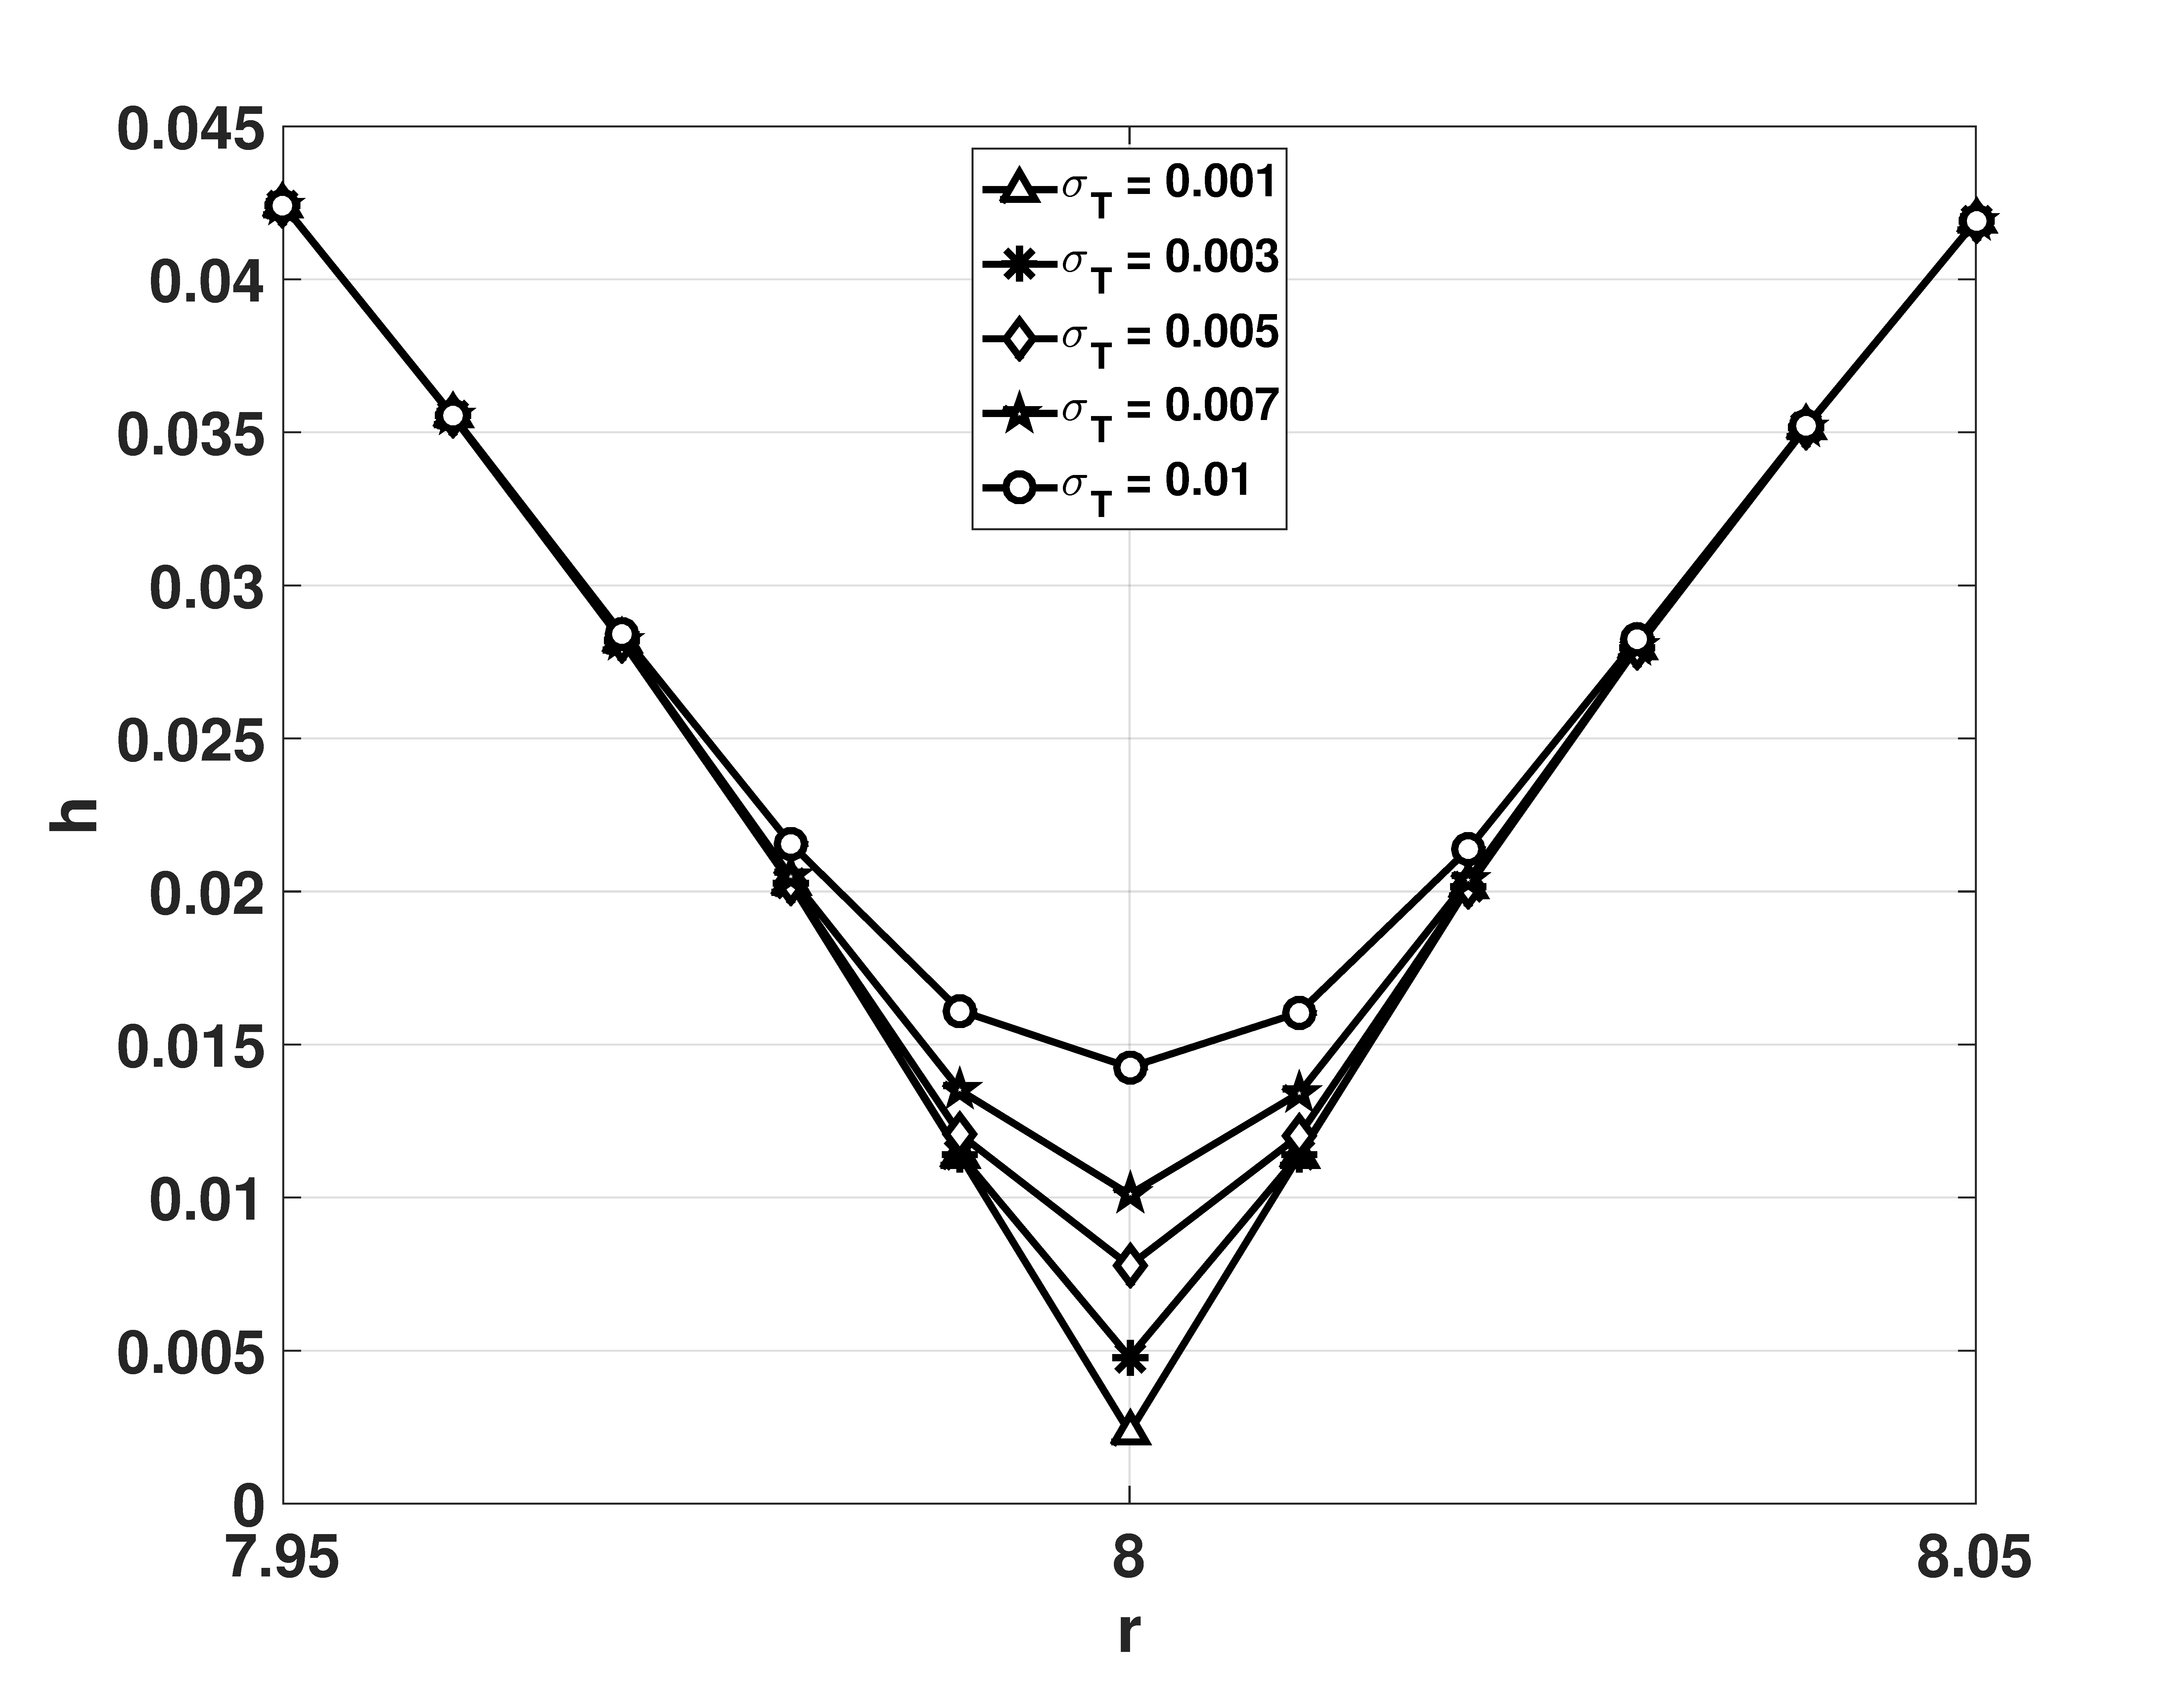
\includegraphics[ width=0.8\textwidth]{h_r_CJ}
\caption{$h$ as a function of $r$ for $r\in[7.95,8.05]$, with several $\sigma_T$ and $W=6$ . The curve has a minimum at the optimum value $r=8$.}
\label{fig:h_r_CJ}
\end{figure}

Further analysis must be done to assure that the selected values $W=6$ and $D=8$ produce symbolic files with a good statistics. For a given alphabet $\mathcal{A}$ with $m$ elements, and a given symbolic file of length $n$, the quality parameter $\alpha=n/m$, see \ref{sec:quanti}. Quality is better as $\alpha$ increases and a minimum value $\alpha=10$ was accepted. According to section \ref{sec:quanti} the selected values $W=6$ and $D=8$ provide $\alpha_h\simeq10^5$, $\alpha_{h^*}\simeq175$ with superposition and $29$ without superposition. All cases give $\alpha>10$ as required.

A comparison between both quantifiers is shown in Figure \ref{fig:hm_h_CJ}. Markers correspond to variances $\sigma_T=\{0,$ $0.001,$ $0.002,$ $0.003,$ $0.004,$ $0.005,$ $0.007,$ $0.01,$ $0.02,$ $0.03,$ $0.04,$ $0.05,$ $0.07,$ $0.1\}$.
Note that the slope of any of these curves is $dh^*/dh$ and it is equal to the quotient between slopes of curves in the insets of Figs. \ref{fig:hm_D_CJ}, and \ref{fig:h_W_CJ}. If $dh^*/dh~>1$, $h^*$ is more sensitive than $h$ to measure jitter. The slope slightly increases from $\sim2.47$ for $W=5$ to $\sim5.54$ for $W=19$ showing that $h^*$ becomes more sensitive as $W$ increases.

\begin{figure}
\center
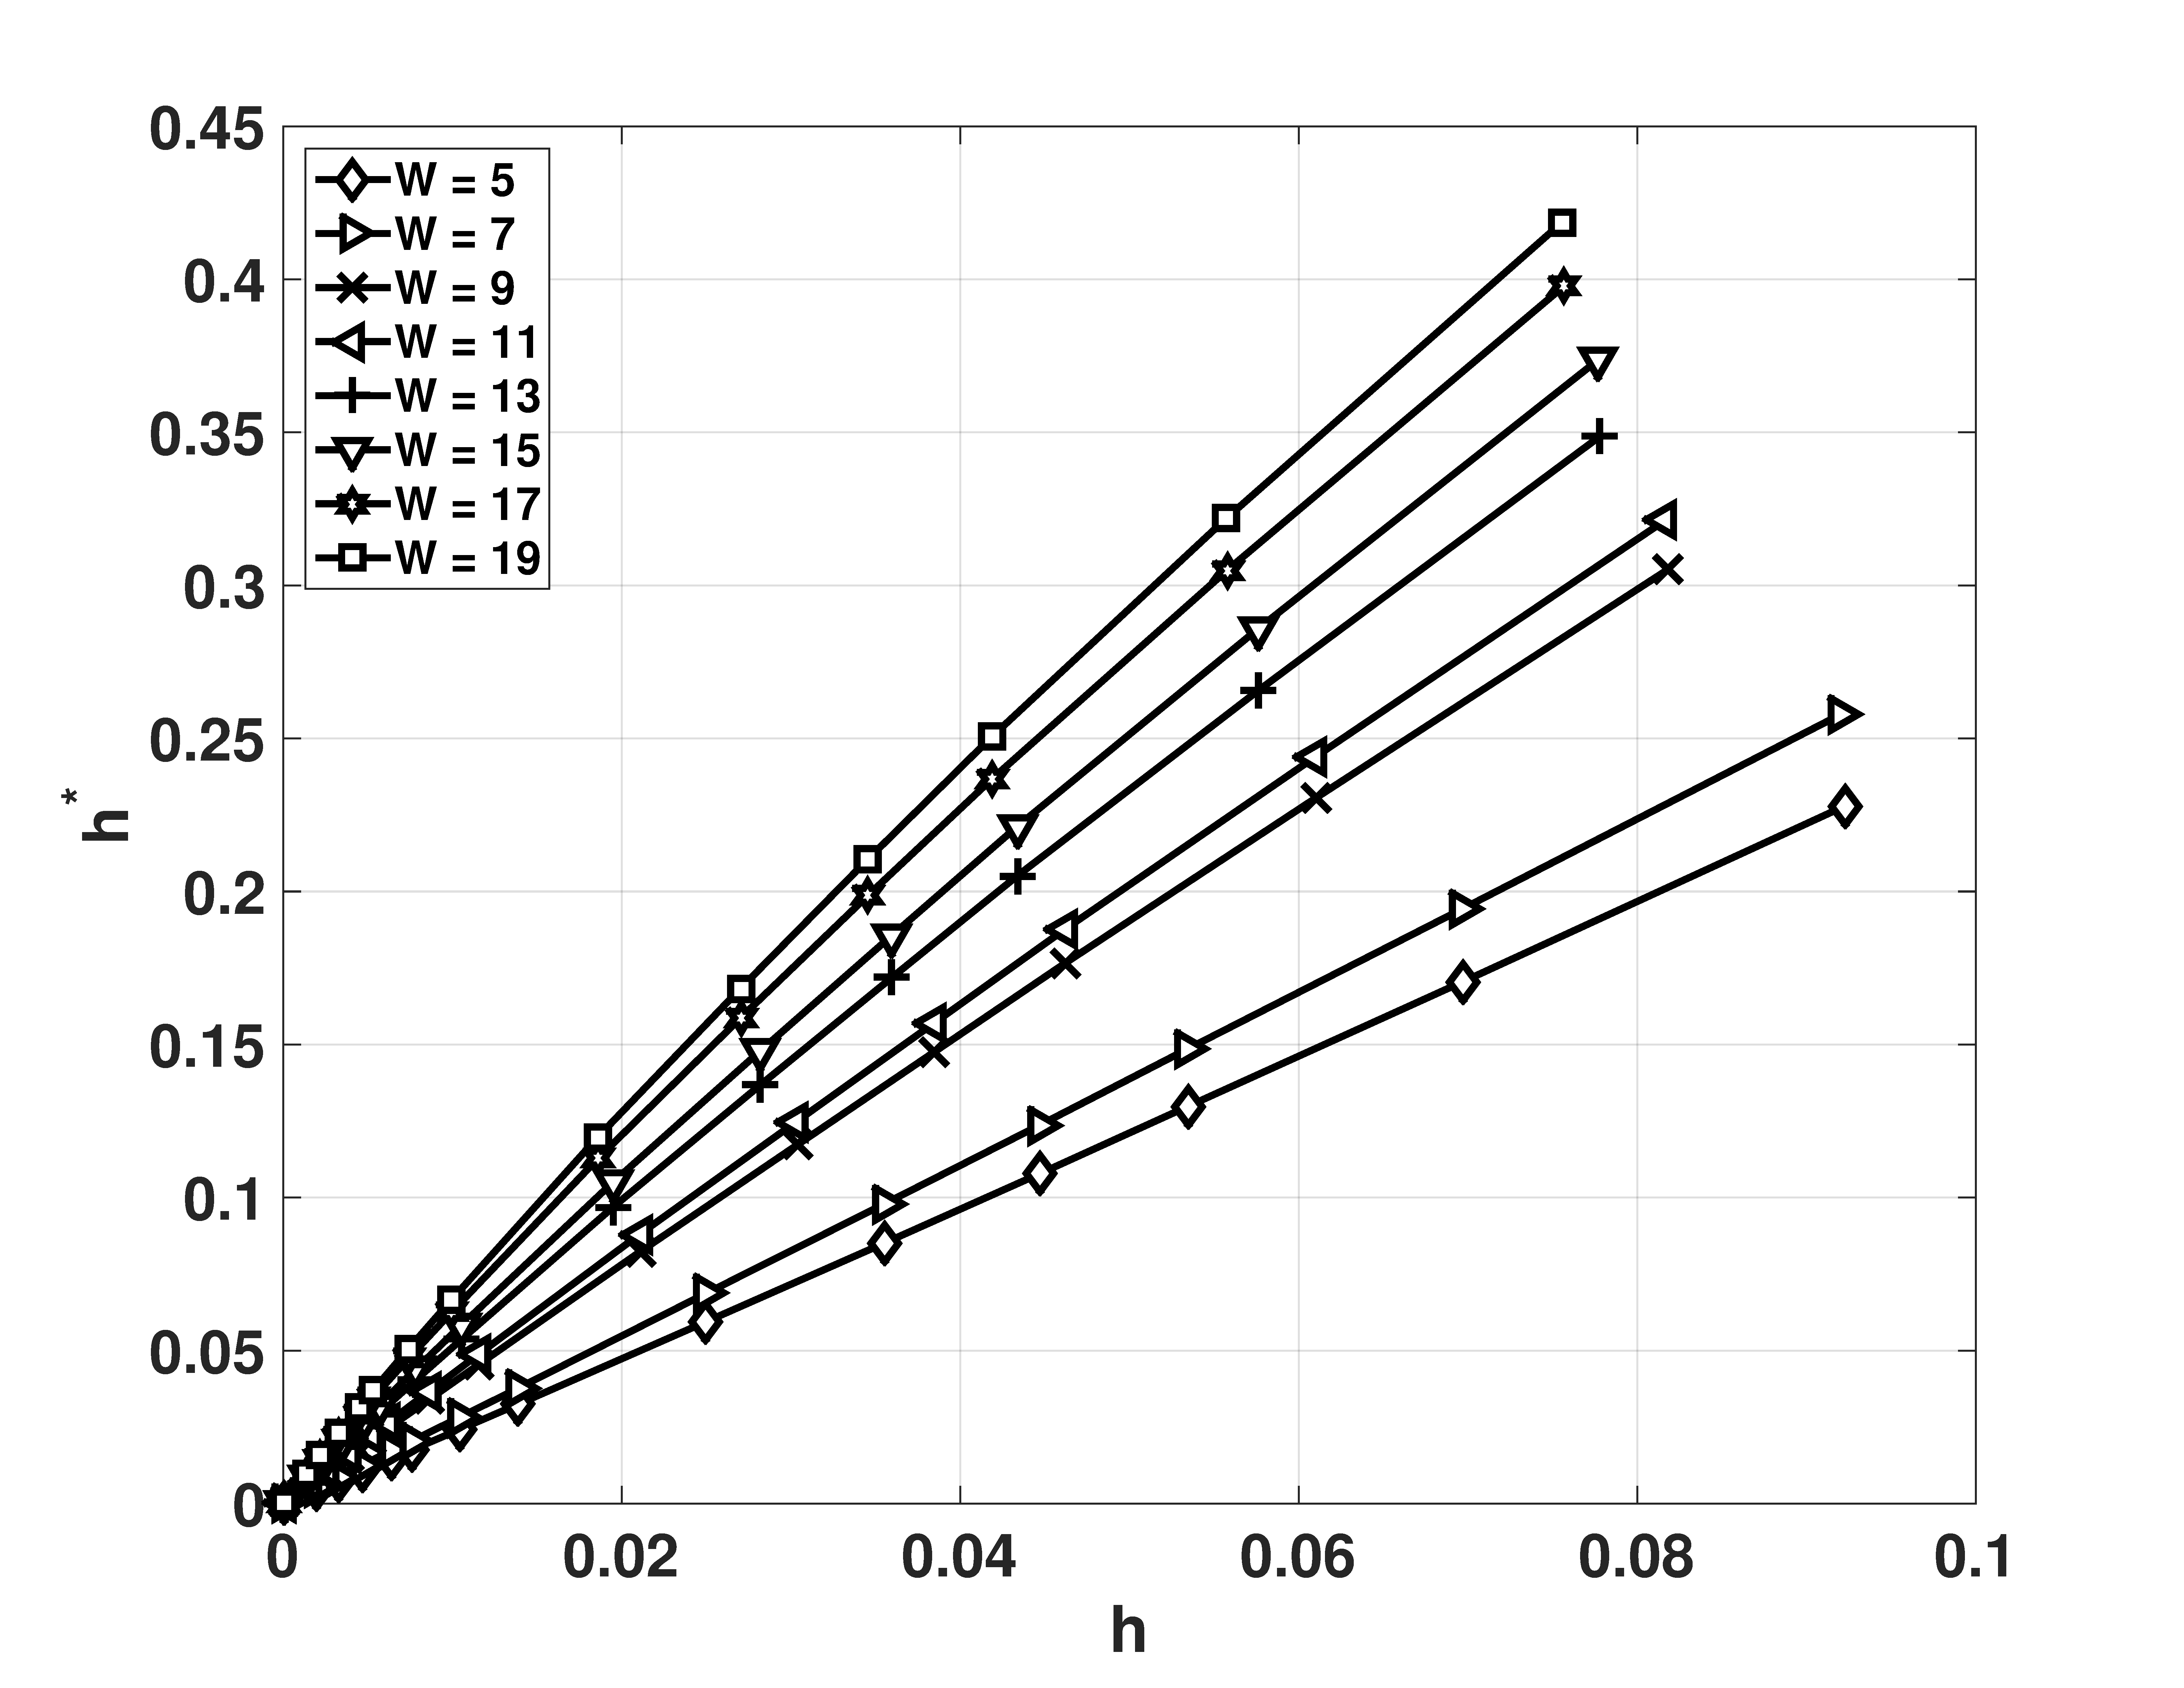
\includegraphics[ width=0.8\textwidth]{hm_h_CJ}
\caption{$h^*$ as a function of $h$ for $r=8$, $D=8$ and different values of $W$.}
\label{fig:hm_h_CJ}
\end{figure}

We also evaluated $h^*$ without the superposition of bits between consecutive natural numbers but keeping the superposition of $D-1$ natural numbers between ordering patterns (In all cases $h$ was evaluated with superposition of $W-1$ consecutive bits). Results are depicted in Fig. \ref{fig:Deltahm_Deltah_CS_SS} where it is shown that removing the superposition the sensitivity of this quantifier increases. Of course, we get a smaller amount of $W$ bits natural numbers form the original seven million binary file, and consequently, the statistical quality is lower than that of the original calculation with superposition. To increase $\alpha$ up to its previous value, longer binary files are required.

\begin{figure}
\center
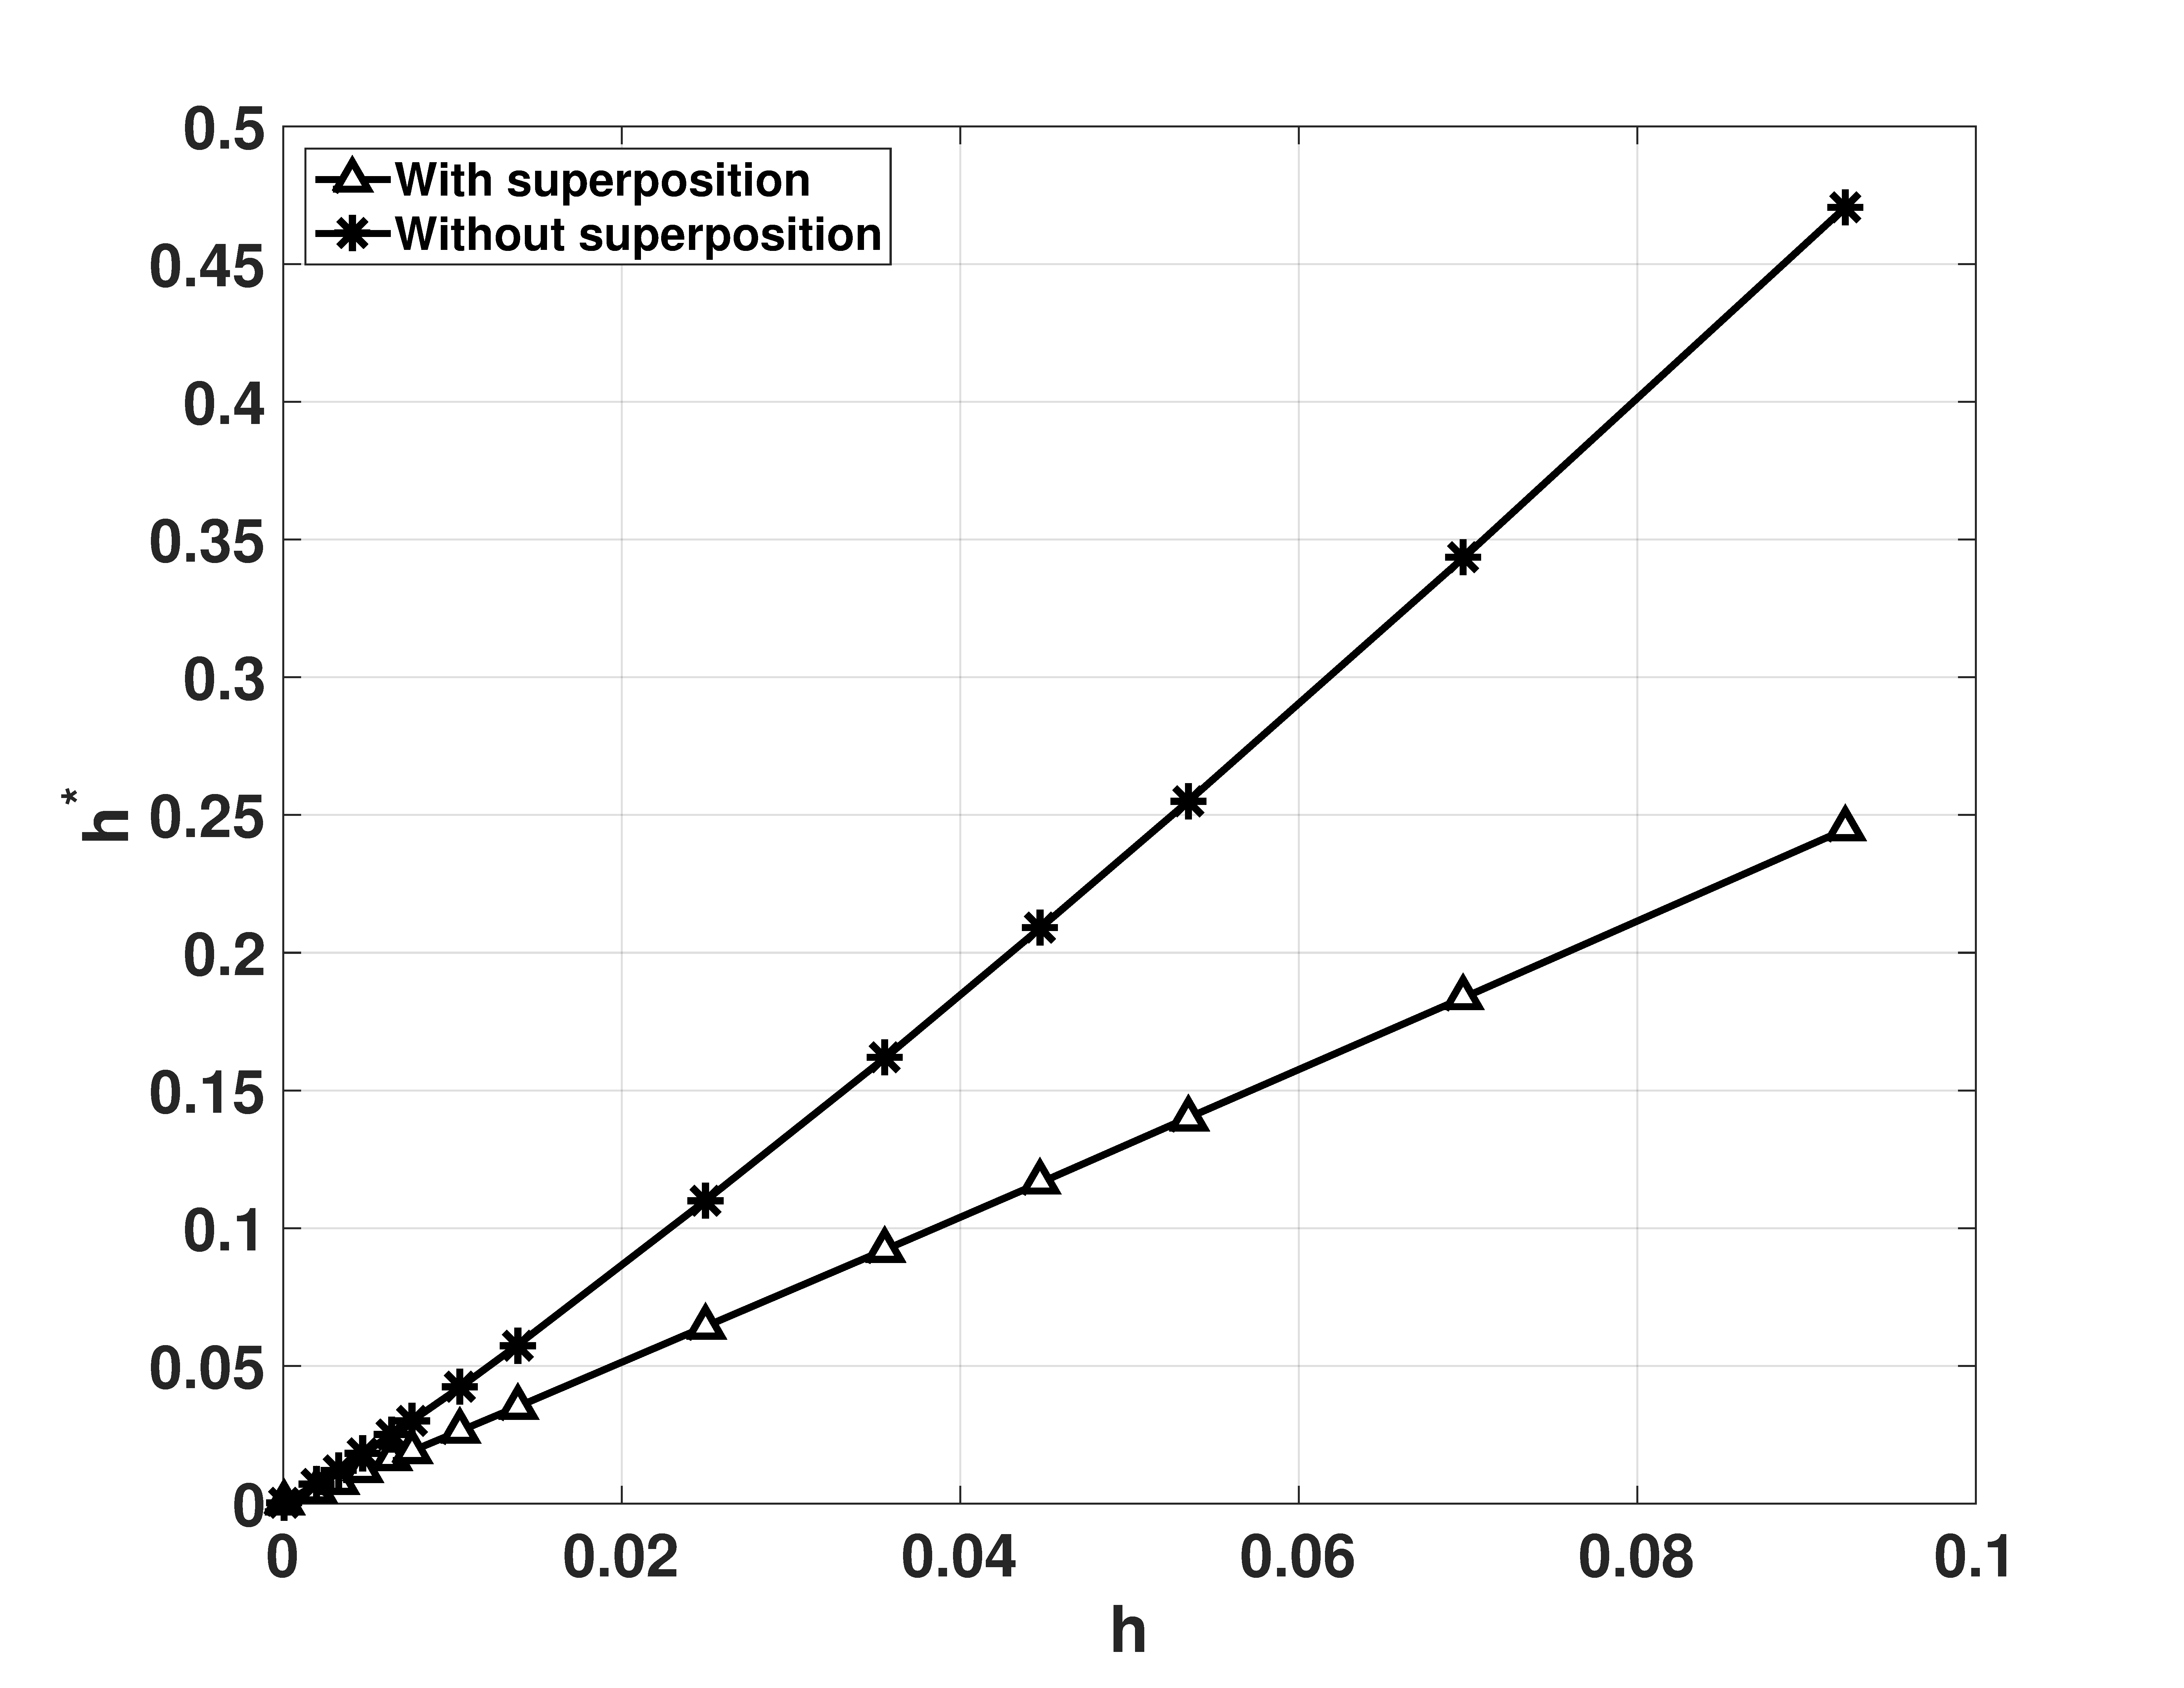
\includegraphics[ width=0.8\textwidth]{Deltahm_Deltah_CS_SS}
\caption{$h^*$ as a function of $h$ for $r=8$, $W=6$ and $D=8$. Two procedures to obtain $W$-bits natural numbers are considered: with and without superposition (see text).}
\label{fig:Deltahm_Deltah_CS_SS}
\end{figure}

\subsection{Conclusions}
\label{sec:conclu}
Given their usefulness as \emph{PRNG} and clock generators, \emph{RO}s are becoming one of the main building blocks of digital circuits. Jitter is unavoidable in \emph{RO}s, and consequently, it needs to be characterized. Mixing and distribution of values are the main properties to consider. 
Several \emph{ITQ} quantifiers were evaluated here. $S_W$, $S^{(D)}_{BP}$, $H_W$ and $H^{(D)}_{BP}$ turn out to be dependent on parameters $W$ and $D$. This is a drawback if we use them as jitter measures. On the other hand, it is no possible to calculate  \emph{rate entropies}, $h_0^*$ and $h_0$,  since an infinite number of data is necessary for their calculation. The two \emph{differential entropies}, $h^*$ and $h$, instead, are independent of the parameters used for their determination and are estimators of the \emph{rate entropies}. We have shown in Section \ref{sec:resu} that in the case of sampled \emph{RO}s they also present a minimum for the correct sampling ratio making them a good measure of the quality of both \emph{RO}'s and \emph{PRNG}'s derived from them. 

The dual entropy plane determined by these quantifiers has demonstrated to satisfactorily discern between the \emph{PRNG}'s two main desired properties, the equiprobability among all possible values and the statistical independence between consecutive values. Thus, it allows clearly seeing what needs to be improved in a given sequence.
The examples presented here have demonstrated the need to use both histograms for characterizing sequences.

%\bibliography{xbibMAXI_300314,xbibwebdiciembre2013_ingles}


%%%%%%%%%%%%%%%%%%%%%%%%%%%%%%%%%%%%%%%%%%%%%%%%%%%%%%%%%%%%%%%%%%%%%%%%%%%%%%%%%%%%%%%%%%%%%%%%%%%%%